%!TEX TS-program = xelatex
%!TEX encoding = UTF-8 Unicode


\documentclass[dsingle]{Dissertate}

\usepackage[vietnamese,english]{babel}
\usepackage{hhline}
\usepackage{subcaption}
%\usepackage{showframe}
% Include other packages here, before hyperref.
\usepackage{algorithm}
\usepackage[noend]{algorithmic}
\usepackage{eqparbox}
\usepackage{sidecap}
\usepackage[labelfont=bf]{caption}
\usepackage[labelfont=it,textfont={it},justification=centering]{subcaption}
\usepackage{comment}
\usepackage{bm}
\usepackage{booktabs}
\usepackage{wrapfig}
\usepackage{textcomp}
\usepackage{xcolor}
\usepackage{threeparttable}
\usepackage[export]{adjustbox}
\usepackage{lipsum}
\usepackage{pgf}
\usepackage{rotating,multirow}
\newcommand*\rot{\rotatebox{90}}
%\usepackage{url}
\usepackage{tikz}
\usepackage{cases}
%\usepackage{subfigure}
\usepackage{longtable}
\usepackage{booktabs}

\renewcommand{\algorithmiccomment}[1]{\hfill\eqparbox{COMMENT}{\# #1}}
% https://stackoverflow.com/questions/1744197/formatting-comments-in-latexs-algorithmic-environment



\def\eg{\emph{e.g}\onedot} \def\Eg{\emph{E.g}\onedot}
\def\ie{\emph{i.e}\onedot} \def\Ie{\emph{I.e}\onedot}
\def\cf{\emph{c.f}\onedot} \def\Cf{\emph{C.f}\onedot}
\def\etc{\emph{etc}\onedot} \def\vs{\emph{vs}\onedot}
\def\wrt{w.r.t\onedot} \def\dof{d.o.f\onedot}
\def\etal{\emph{et al}\onedot}


\makeatletter
\newcommand\footnoteref[1]{\protected@xdef\@thefnmark{\ref{#1}}\@footnotemark}
\makeatother


\def\-{\raisebox{.75pt}{-}}
\DeclareMathOperator*{\argmax}{argmax}
\DeclareMathOperator*{\argmin}{argmin}

\def\httilde{\mbox{\tt\raisebox{-.5ex}{\symbol{126}}}}



\begin{document}

% the front matter
%!TEX root = ../dissertation.tex
% Some details about the dissertation.
\title{You can have multiple titles}
\title{and have them listed here for considering}
\title{but the only one counted is the last and }
\title{Fancy title of your thesis \\ \Large together with its subtitle}
\author{My Name}
\phdfrom{My Birth City} % only city, not country, from the Beadle Office
\defendVenue{[Aula der Universiteit/Agnietenkapel*]}

\defendDOW{d.o.w}               % dinsdag day of week, in Dutch
\defendDay{[...day...]}         % 18
\defendMonth{[...month...]}     % mei (in Dutch)
\defendYear{202[...]}           % 2021 
\defendTime{[...time...]}       % 12:00


%If you have one advisor
\advisor{prof. dr. supervisor}
\advisorSchool{Universiteit van Amsterdam}

\coadvisor{dr. co-supervisor}
\coadvisorSchool{\begin{tabular}[t]{@{}l@{}}Universiteit van Amsterdam \\Google Research\end{tabular}\\ }
\advisorSchool{Universiteit van Amsterdam}

\committeeOne{prof. dr. committee member 1}
\committeeOneSchool{Universiteit van Amsterdam}
\committeeTwo{prof. dr. committee member 2}
\committeeTwoSchool{Universiteit van Amsterdam}
\committeeThree{prof. dr. committee member 3}
\committeeThreeSchool{Universiteit van Amsterdam}
\committeeFour{dr. committee member 4}
\committeeFourSchool{Universiteit van Amsterdam}
\committeeFive{dr. committee member 5}
\committeeFiveSchool{Universiteit van Amsterdam}


\definecolor{SchoolColor}{rgb}{0.3412, 0.0235, 0.5490} % purple 
\definecolor{chaptergrey}{rgb}{0.2600, 0.0200, 0.4600} % dialed back a little   
\definecolor{midgrey}{rgb}{0.4, 0.4, 0.4}


    \frontmatter
    \setstretch{\dnormalspacing}

    \AddLabels % for chapterthumbs
    \graphicspath{{figures/}}

\pagestyle{fancy}
\fancyhead[LO,RE]{}
\fancyhead[LE]{\leftmark}
\fancyhead[RO]{\rightmark}

\renewcommand\chaptermark[1]{\markboth{\MakeUppercase{\thechapter. #1}}{\MakeUppercase{\thechapter. \small #1}}}
%\renewcommand\sectionmark[1]{\markright{#1}}

%!TEX root = ../dissertation.tex

\begin{savequote}[65mm]
An inspiring quote to start the chapter
\qauthor{Somebody}
\end{savequote}

\chapter{Introduction}
\label{chap:intro}p

\lettrine[lines=3]{\textcolor{SchoolColor}{A}}{bstract of the chapter is here}.tp
More to be written here.
\lipsum[1]

\section{Introduction}
yp
\lipsum[3-5]t
\cite{1}
%!TEX root = ../dissertation.tex

\begin{savequote}[75mm]
Another inspiring quote for this chapter
\qauthor{Another author maybe}
\end{savequote}


\chapter[High-performance computing in healthcare: An automatic literature analysis perspective]{High-performance computing in healthcare: An automatic literature analysis perspective}

\lettrine[lines=3]{\textcolor{SchoolColor}{T}}{%bstract of the chapter could go here
}
he adoption of high-performance computing (HPC) in healthcare has gained significant attention in recent years, driving advancements in medical research and clinical practice. Exploring the literature on HPC implementation in healthcare is valuable for decision-makers as it provides insights into potential areas for further investigation and investment. However, manually analyzing the vast number of scholarly articles is a challenging and time-consuming task. Fortunately, topic modeling techniques offer the capacity to process extensive volumes of scientific literature, identifying key trends within the field. This paper presents an automatic literature analysis framework based on a state-of-art vector-based topic modeling algorithm with multi-embedding techniques, unveiling the research trends surrounding HPC utilization in healthcare. The proposed pipeline consists of four phases: paper extraction, data preprocessing, topic modeling and outlier detection, followed by visualization. It enables the automatic extraction of meaningful topics, exploration of their interrelationships, and identification of emerging research directions in an intuitive manner. The findings highlight the transition of HPC adoption in healthcare from traditional numerical simulation and surgical visualization to emerging topics such as drug discovery, AI-driven medical image analysis, and genomic analysis, as well as correlations and interdisciplinary connections among application domains.

\section{Introduction}\label{se:2-1}

High Performance Computing (HPC) is increasingly becoming an indispensable resource in healthcare research due to its capabilities in addressing complex and data-intensive tasks~\cite{elsebakhi2015large,raj2015big,jia2014gpu}. The exponential growth of health data next to simulation and modeling drives the adoption of HPC, which encompasses i.a., genomic sequencing, biomedical imaging, electronic health records (EHRs), and wearable device data \cite{bastrakov2013high,schmidt2017next,stocker2010high,alanazi2015meeting,vitabile2019medical}. Effectively managing and analyzing such data poses significant challenges in storage, management, and analysis, necessitating the computational power offered by HPC. In genomics, HPC allows researchers to analyze genomic data at a scale and speed previously impossible, revealing genetic bases of various diseases and helping develop personalized treatments~\cite{molidor2003new,lightbody2019review}. Similarly, HPC plays a crucial role in drug discovery and computational modeling  \cite{CHEN20181241,jumper2021highly}.
Drug discovery processes are traditionally time and resource-intensive. However, HPC allows researchers to conduct molecular dynamics simulations to understand drug-protein interactions at the atomic level, speeding up the process and reducing costs~\cite{zhang2014toward,ge2013molecular,sanbonmatsu2007high}. Furthermore, HPC-enabled computational modeling allows the simulation of biological systems or disease progression, providing insights to inform treatment strategies~\cite{kharche2008simulation,perrin2010model}. The deployment of HPC in Artificial Intelligence (AI) for healthcare has also experienced substantial growth. HPC enables the implementation of advanced AI techniques, which necessitate substantial computational power to efficiently handle extensive data volumes and complex deep neural networks~\cite{phong2017brain,cirillo2019big}. Biomedical imaging stands as a prime example where HPC assumes a crucial role \cite{LITJENS201760}. By leveraging HPC, AI tools can swiftly process and analyze high-resolution images, facilitating real-time analysis of complex imaging data and leading to expedited and more precise diagnoses~\cite{cai2020review,tahmassebi2018deep}. In addition, HPC-enabled convergence of AI and simulation has significantly improved the quality and speed of traditional simulation in healthcare~\cite{lee2019deepdrivemd,bai2022application}. 

Investigating the literature on HPC adoption in healthcare can generate valuable insights that are beneficial for the business and economic side of healthcare by providing a comprehensive understanding of the current landscape and potential future directions. These insights can guide strategic planning and investment decisions of HPC in healthcare businesses, highlighting promising areas for further exploration and development. However, the substantial volume of literature, combined with the rapid pace of technological advancements, makes manual analysis very difficult and time consuming. As a result, there is a recognized need for an automated literature analysis framework to accurately process the vast corpus of literature, transforming it into meaningful insights for business or strategic decision making within the healthcare sectors.

Topic modeling, a family of typically unsupervised machine learning approaches, aims at discovering hidden semantic structures, or `topics', within a corpus of text~\cite{blei2012probabilistic}. The underlying principle of topic modeling is to classify text documents into different topics based on the frequency and co-occurrence of words~\cite{jacobi2018quantitative}. The strength of topic modeling lies in its capacity to handle large and unstructured datasets, rendering it an invaluable tool for exploratory data analysis. Prominent techniques employed in topic modeling include Latent Dirichlet Allocation (LDA)~\cite{blei2003latent}, Non-negative Matrix Factorization (NMF)~\cite{lee1999learning}, and Latent Semantic Analysis (LSA)~\cite{deerwester1990indexing}. With a broad range of applications in areas such as text mining, information retrieval, and digital humanities, topic modeling continues to garner considerable interest~\cite{alghamdi2015survey,yi2009comparative,meeks2012digital}. Topic modeling has become an increasingly popular tool in scientific research and literature review~\cite{asmussen2019smart,amado2018research,chen2019identify}. Its usage spans various scientific research fields, including marketing, medical, and social sciences~\cite{amado2018research,algaa2020analysis,lindstedt2019structural}. In the context of literature reviews, topic modeling has been used to identify trends and patterns in large bodies of literature. For instance, it has been used to analyze collective behavior and social movements by sociologists~\cite{lindstedt2019structural}, and also been adopted to understand the big data themes from biomedical research~\cite{van2016understanding}. 

LDA is arguably one of the most widely used algorithms for topic modeling. However, it has been characterized by certain constraints, including the prerequisite of data cleaning and pre-processing, the requirement to specify model parameters such as $\alpha$ (document-topic density), $\beta$ (topic-word density) and topic numbers hyperparameters. Moreover, the challenges associated with the interpretability and validation of the generated topics also need to be addressed~\cite{maier2018applying,angelov2020top2vec}, which is why alternatives such as entity linking (EL) have been frequently deployed, especially in case of shorter texts \cite{10.1145/3126686.3126776}. In response to these limitations, recently developed deep learning algorithms such as Top2Vec, offer alternative approaches for topic modeling~\cite{angelov2020top2vec}. Top2Vec transforms each word in a text collection into a vector representation within a semantic space using an encoding model such as doc2vec or state of the art transformers. Consequently, it autonomously identifies topics within the text and generates jointly embedded topic, document, and word vectors. Comparative studies between LDA and Top2Vec have been conducted, revealing that Top2Vec tends to yield qualitatively superior results compared to LDA~\cite{egger2022topic,karas2022experiments}.

In this study, we propose an automatic literature analysis framework, using a complex question of the impact of HPC on healthcare as the test-bed. The primary contributions of this work are twofold:

\begin{enumerate}
\item We present an automatic literature analysis framework, from document (i.e. scientific article) retrieval and analysis to various interactive visualizations to depict research trends, topics evolution, interconnection across research areas and high impact papers. This adaptable pipeline can be easily applied to other domains by modifying the initial query keywords.
\item By deploying the automated literature analysis framework, we investigate the research trends of HPC utilization in healthcare. Our analysis reveals notable shifts in research focus, spanning from visualization and rendering in surgical practice and traditional numerical simulation to emerging topics such as drug discovery, AI-driven medical image analysis, and genomic analysis. These insights provide valuable indications for future investment and strategic development of HPC within the healthcare sector, guiding decision-making and resource allocation.
\end{enumerate}

\section{Materials and methods}\label{se:2-2}

In this section, we provide a comprehensive description of the data and analysis process employed in our study. Figure~\ref{fig:2-1} illustrates the automatic literature review framework implemented in our study, which consists of four distinct stages: paper retrieval and extraction, data preprocessing, topic modeling, and visualization. The subsequent sections provide detailed explanations of each stage.
\begin{figure}[!h]
\centering
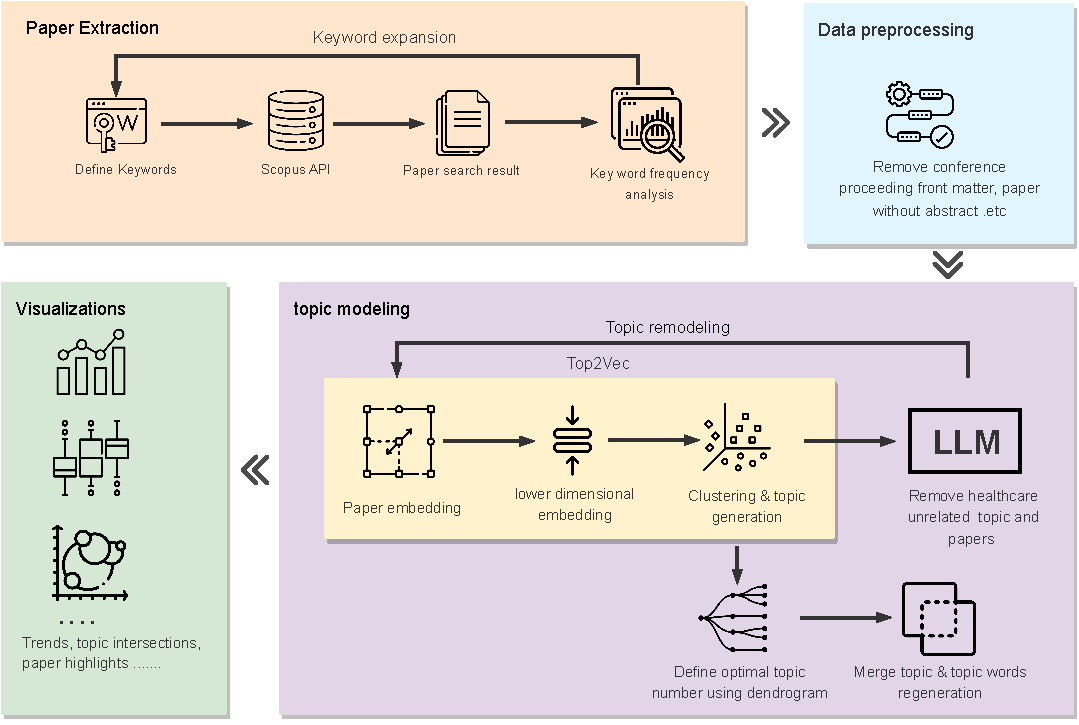
\includegraphics[width=0.9\textwidth]{2-1.pdf}
\caption{Automatic literature review pipeline consists of four stages: paper retrieval and extraction, data preprocessing, topic modeling, and visualization}
\label{fig:2-1}
\end{figure}


\subsection{Paper retrieval and extraction}\label{subse:2-2.1}
\subsubsection{Data source}\label{subsubse:2-2.1.1}

Scopus\footnote{\url{https://www.elsevier.com/solutions/scopus}}  has been utilized in our study as it is the largest publicly available abstract and citation database of peer-reviewed literature, including scientific journals, books and conference proceedings.

\subsubsection{Type of articles included in the study}\label{subsubse:2-2.1.2}

In this study, conference papers, journal papers, books or book chapters, editorial materials, early access workshop papers and presentations published in English are included. Conference proceeding front matters, meeting abstracts, errata and papers without abstracts are excluded from the analysis. Since the publication year 2023 is not yet complete, studying trends beyond 2022 may introduce bias. Therefore, we limit our analysis to publications up until end of 2022.



\subsubsection{Paper retrieval pipeline}\label{subsubse:2-2.1.3}

We establish an automatic paper record retrieval and query expansion pipeline through the Scopus API\footnote{\url{https://dev.elsevier.com/}}. During the initial phase of query construction, we take into account the co-occurrence of HPC keywords such as `high performance computing' and `supercomputing' along with the most prevalent health-related terms like `healthcare', `health', `clinic',`medicine', `disease', and `treatment'. With each iteration of the literature search, we implement query expansion by incorporating additional relevant keywords extracted from the retrieved scientific paper documents. To achieve this, we perform a frequency analysis of keywords extracted from the titles and abstracts. Keywords that are identified as HPC or healthcare-related and occur with a frequency of 50 or higher, but are not previously included, are considered as new keywords and subsequently added to the expanded query. Such automatic query expansion process results in inclusion of the synonyms of HPC, such as `high-performance computing', `high performance computer', and `supercomputer', along with broader or narrower healthcare-related terms like `patient', `diagnosis', `drug', `therapy', `pharmaceutical', `surgery', and others. This process is repeated until no new keywords emerge, indicating the completion of the search query expansion. The extracted literature serves as an input for further processing in the subsequent steps.


\subsection{Data preprocessing}\label{subse:2-2.2}
Based on the output obtained from Scopus, we retain the title, abstract, publication date, and citation number for subsequent topic modeling and visualization. Given that the Top2Vec algorithm does not require stop-word lists nor stemming, or lemmatization, the title and abstract of each literature piece are merged as the model input without further preprocessing.
\subsection{Topic Modeling }\label{subse:2-2.3}

\subsubsection{Algorithm choice}\label{subsubse:2-2.3.1}

We adopt the Top2Vec model for topic modeling, an innovative unsupervised machine learning algorithm designed for automatic topic detection and document embedding~\cite{angelov2020top2vec}. This model is unique as it combines the strengths of word embeddings, dimensionality reduction, and density-based clustering to identify topics from a given set of documents without any prior knowledge or human intervention.

The first step in the Top2Vec algorithm involves transforming the documents into dense vector representations using chosen embedding algorithm to capture the semantic meanings of the documents, including the context in which words are used, and represents them as high-dimensional vectors. This process results in a document embedding space where semantically similar documents are located close to each other. We process the input literature by employing five distinct embedding techniques available in the Top2Vec algorithm to generate combined document and word vectors. These techniques include doc2vec~\cite{le2014distributed}, two Universal Sentence Encoder models~\cite{cer2018universal,yang2019multilingual}, and two BERT models~\cite{reimers2019sentence,reimers2020making}. We implement the CV coherence score in our topic modeling evaluation, a metric initially introduced by R?der et al. in their comprehensive examination of coherence measures for topic modeling algorithms~\cite{roder2015exploring}. The CV coherence score combines cosine similarity with Normalized Pointwise Mutual Information (NPMI). This selection is premised on the strong correlation that the CV coherence score maintains with human ratings, outperforming other evaluative measures. Consequently, we choose the embedding model demonstrating the highest CV coherence score for our study. 

Once the documents are represented as vectors, the Top2Vec model applies the UMAP (Uniform Manifold Approximation and Projection) algorithm to reduce the dimensionality of these vectors~\cite{mcinnes1802umap}. UMAP is a manifold learning technique used for dimension reduction. It preserves both the local and global structure of the data, meaning that it maintains the distances between nearby points (local structure) and distant points (global structure). This results in a lower-dimensional space where clusters of document vectors represent unique topics. 

Following the dimensionality reduction, the model uses HDBSCAN (Hierarchical Density-Based Spatial Clustering of Applications with Noise), a density-based clustering algorithm, to identify these clusters~\cite{campello2013density}. HDBSCAN works by finding regions of the reduced space where there are higher densities of document vectors, and it groups these together as clusters. Each cluster represents a unique topic in the document set and the centroid of each cluster is identified as a `topic vector'. This topic vector is a point in the reduced space that best represents the semantic meaning of each topic. The topic vectors are then transformed back into the word space to provide interpretable topics. This is done by finding the words that are most similar to each topic vector, which are then used as the keywords for the topic. One of the key advantages of the Top2Vec model is that it automatically determines the optimal number of topics based on the data. Additionally, it provides both the keywords for each topic and the documents that are most semantically similar to each topic, offering a comprehensive understanding of the topics present in the document set.


\subsubsection{Identify outlier topics not focusing on HPC adoption in healthcare and remodeling}\label{subsubse:2-2.3.2}
During the literature extraction process, articles that contain healthcare and high-performance related keywords within the title, abstract, or keyword sections are extracted via the Scopus API. However, initial topic modeling results reveal that certain articles do not relate to HPC adoption in healthcare. This discrepancy can be attributed to multiple factors. Firstly, while some articles include the terms `high performance computing' and `health' or `healthcare' in their titles or abstracts, they predominantly address aspects of system health such as fault tolerance, job scheduling, and interconnection, rather than human health. This results in these articles being categorized under topics such as system architecture or networks. Secondly, many abstracts begin with a broad statement, such as ``high-performance computing has been widely used in several industries, including healthcare ...'' but the remainder of the abstract primarily discusses the adoption of HPC in domains other than healthcare. 

The GPT-3 series model has demonstrated promising results in binary semantic text classification~\cite{zografos2023gpt}. To fully automate our analysis pipeline and minimize potential bias from human judgment, we employed \texttt{text-davinci-003}, the most advanced model in the GPT-3 series, for non-healthcare related topic detection. Similar to studies~\cite{carpenter2023using,bommarito2022gpt}, following the first round of topic modeling that generates keywords, we design prompts using \texttt{the text-davinci-003} text completion API\footnote[2]{https://platform.openai.com/docs/models/gpt-3-5}. These prompts incorporate the top 20 keywords from each topic, aiming to produce binary outputs that determine whether the keyword combination for each topic pertains to the healthcare domain. To align with our expectation of binary output (\texttt{Yes} or \texttt{No}), we adjust the \texttt{max\_tokens} parameter indicating the upper limit of tokens to be generated, to a smaller value of 5. The \texttt{temperature}  parameter is set to 0 to limit the randomness of the generated responses, ensuring a more focused and deterministic output.  All other hyperparameters are retained at their default values. If a topic is classified as unrelated to healthcare, the articles under that topic are identified as outliers and removed from the dataset. Once all topic keywords have been examined, the remaining literature proceed to the second round of topic modeling.

\subsubsection{Identify optimal topic number using dendrogram}\label{subsubse:2-2.3.3}

Upon evaluating the preliminary output from the Top2Vec model after the outlier detection phase, we observe that certain topics demonstrate substantial similarity and an increased granularity. Examples include multiple themes associated with virus and epidemic research, genomic research, and drug discovery (cf. Section \ref{subse:2-3.2} and Figure~\ref{fig:2-2} for detailed observations). Merging similar topics to identify an optimal topic number could prove beneficial in subsequent analysis, providing a more overarching perspective on HPC adoption trends in healthcare.

Agglomerative hierarchical clustering with dendrogram is a technique used to aggregate similar data points or objects into clusters based on their pairwise distances~\cite{nielsen2016hierarchical}. This technique initiates with individual data points and sequentially merges these based on their proximity relationships. For the computation of similarities between topic vectors, cosine similarity has been utilized. This measure proves to be particularly beneficial when processing high-dimensional data, such as semantic word embeddings~\cite{orkphol2019word,rozado2019using}. Cosine similarity takes into account both the magnitude and direction of each vector, property making it more robust compared to the common alternatives like Euclidean distance, which considers only the magnitude. In the context of our hierarchical clustering, we have adopted the average linkage method~\cite{nielsen2016hierarchical}.

The outcome is a dendrogram that displays hierarchical relationships. The methodology starts with the calculation of a distance matrix that captures the distances between topic vectors. The closest clusters are sequentially merged, and the distances are updated correspondingly. The dendrogram is constructed to portray the merging process, with branch lengths representing dissimilarity. By studying the dendrogram, an appropriate cutting point can be identified to determine the number of clusters. Hierarchical clustering provides a comprehensive visualization and organization of topics, aiding in understanding its inherent structure and interrelationships. Therefore, dendrogram has been utilized to visualize the topic merging process and to determine the optimal topic number.


\subsubsection{Topic merging}\label{subsubse:2-2.3.4}

Having determined the optimal number of topics using the dendrogram, we proceed to consolidate the topics. Top2Vec provides a function \texttt{hierarchical\_topic\_reduction} designed to decrease the number of topics identified by the algorithm\footnote[3]{https://github.com/ddangelov/Top2Vec}. However, the process operates by iteratively merging the smallest topic based on the number of associated documents with the most similar topic until the predetermined number of topics is reached. We conjecture that this approach, which prioritizes the size of the topics rather than their similarity for merging, may not be optimal. Specifically, the topic associated with the smallest cluster of documents in each merging iteration could represent an emergent topic, potentially displaying considerable divergence from other topics. Thus, merging topics based primarily on their sizes could introduce bias into the process. Therefore, in line with the methodology of agglomerative hierarchical clustering, we advocate for an iterative merging of topics based primarily on their similarity, rather than their respective sizes.

\subsection{Visualization }\label{subse:2-2.4}


\subsubsection{Visualizing the trends of HPC adoption in healthcare based on application domain}\label{subsubse:2-2.4.1}


To visualize trends of HPC adoption in healthcare, we employ four types of graphical representations: Word clouds, stacked area charts, normalized stacked area charts, and violin plots. Before proceeding with visualization, we again utilize the \texttt{text-davinci-003} model via the OpenAI API to summarize the topic in less than 10 words based on the top 20 keywords extracted from each topic.

As a variant of the classic area chart, stacked area chart partitions the area into segments, each representing a specific topic. The \texttt{x-axis} denotes the publication years, and the \texttt{y-axis} represents the cumulative count of publications. The thickness of each segment within a given year directly corresponds to the number of publications for that particular topic. This not only allows for an easy understanding of the distribution of individual topics over time but also visualizes the total volume of publications for each year. Additionally, the normalized stacked area chart effectively highlights the comparative size of each topic within the overall research landscape, enabling the identification of shifts in academic concentration across time. It provides a comprehensive, aggregate perspective of topic prevalence over the years, underlining research trend evolution.

The violin plot serves as another efficient visualization tool for presenting the trends of publication based on topics across different publication years. It merges the attributes of a box plot and a kernel density plot to provide a comprehensive view of the data distribution.  The `violins' broadness represents the density of publications, facilitating an intuitive comprehension of the prevalent topics for a specific year. It provides an intuitive comparison of publication activity across multiple topics and years, providing insights into the transformation of scholarly focuses over time.


\subsubsection{Visualizing the correlation and convergence of topics}\label{subsubse2.4.2}

In our study, we capitalize on the UMAP generated by Top2Vec and adapt it to produce an interactive bubble chart to illustrate the correlation and convergence of topics. Given that UMAP reduces the high-dimensional document vectors to a two-dimensional space, the similarity of each document within a given topic is depicted by their proximity in this visual representation. Furthermore, we choose to symbolize the centroid of each topic with a triangle marker and prominently feature the top three most-cited papers from each topic for subsequent reading and analysis. To effectively illustrate the correlation and convergence among various topics, we construct a circle centered at the centroid of each topic, encompassing 70\% of the literature associated with the topic. The areas of overlap among these circles serve as indicators of potential convergence across diverse topics.

\section{Results}\label{se:2-3}

In the results section, we first compare different embedding models utilized within the top2vec algorithm, highlighting the performance differences and selecting the most fitting model for our data. Secondly, the process of topic merging is delineated through dendrograms, guiding the optimal selection of the number of topics. This is further complemented by visualizing the trends of HPC adoption in healthcare applications through an array of graphical representations including word clouds, stacked area charts, normalized stacked area charts, and violin charts. The correlations and convergence of topics are further explored through bubble charts. providing insights into the inter-relationships between different subject areas. Finally, through all the analysis results mentioned previously, we engage in an in-depth discussion of what we have learned from the past and present of HPC adoption in healthcare to identify its future strategic opportunities. This sets the stage for a comprehensive understanding of the evolution and potential of HPC in the healthcare domain.



\subsection{Embedding model comparison results}\label{subse:2-3.1}

As described in section \ref{subsubse:2-2.3.1}, we use CV coherence score to evaluate five embedding models. As shown in Table \ref{tab:2-1}, the Doc2Vec model achieves the highest coherence score of 0.622. This is followed by the Universal Sentence Encoder Large model with a score of 0.423, the Universal Sentence Encoder Multilingual Large model with 0.391, the all-MiniLM-L6-v2 model scoring 0.351, and lastly the paraphrase-multilingual-MiniLM-L12-v2 model with 0.332. Based on these outcomes, the Doc2Vec model is chosen as our default embedding model for Top2Vec due to its superior performance.

\begin{table}[!h]
\centering
\caption{Embedding model evaluation results}
\label{tab:2-1}
\setlength{\tabcolsep}{0.8mm}{
\begin{tabular}{lll}
\toprule
Embedding model & Model types & CV coherence \\
\midrule
doc2vec & doc2vec & \textbf{0.622} \\ 
universal sentence 
encoder large & universal sentence 
encoder & 0.423 \\ 
universal sentence
encoder multilingual
large & universal sentence 
encoder & 0.391\\
all-MiniLM 
L6-v2 & BERT & 0.351\\ 
paraphrase-multilingual
MiniLM-L12-v2 & BERT & 0.332\\
\bottomrule
\end{tabular}}
\end{table}


\subsection{Visualizing the process of topic merging using dendrograms for optimal topic number selection}\label{subse:2-3.2}

As described in section \ref{subsubse:2-2.3.3}, we employ a dendrogram to intuitively determine the optimal number of topics by visualizing the merging process of agglomerative hierarchical clustering. As presented in Figure~\ref{fig:2-2}, Top2Vec automatically generates 24 topics during the initial round of topic modeling. Each merging point marks the residual number of topics after the merging process. Among these, six topics are related to genomics analysis (as shown in the top six topics on the dendrogram), two topics pertain to epidemic and virus research, and two are associated with drug discovery. To effectively illustrate the primary trends of HPC adoption in healthcare, we identify an appropriate cut-off at the eleven topics (indicated by a grey vertical dashed line) and proceeded to consolidate similar topics.

\begin{figure}[!h]
\centering
\includegraphics[width=1.0\textwidth]{2-2.eps}
\caption{Dendrogram of hierarchical clustering with Identified optimal topic number}
\label{fig:2-2}
\end{figure}

\subsection{Trends of HPC adoption in healthcare Applications}\label{subse:2-3.3}


Figure~\ref{fig:2-3} illustrates word clouds for eleven distinct topics, derived from the merging process. Each sub-word cloud's title serves as a summary of the topic words, which are generated by the \texttt{text-davinci-003} model as discussed in Section \ref{subsubse:2-2.4.1}. The identified topics include `Healthcare ICT infrastructure', `Genomic Analysis', `Numerical simulation of blood flow and cardiology', `Drug Discovery', `Deep learning medical image analysis', `Medical imaging registration \& reconstruction', `Surgery visualization and rendering', `Epidemic research', `Neuroscience and brain activity analysis', `Radiation Therapy Planning', and `Elderly patient surgical risk and outcome'.

\begin{figure}[!h]
\centering
\includegraphics[width=1.0\textwidth]{2-3.png}
\caption{Word clouds of eleven topics derived from Top2Vec. The main application domains include genomic analysis, drug discovery, medical image analysis, surgery visualization and epidemic research.}
\label{fig:2-3}
\end{figure}

As indicated by the stacked area chart and normalized stacked area chart in Figure~\ref{fig:2-4} and Figure~\ref{fig:2-5}, the utilization of HPC in healthcare has seen significant growth over the past four decades. Based on the data extracted from Scopus, the pioneering paper highlighting HPC's contribution to healthcare, specifically the rapid analysis of long electrocardiogram (ECG) records, was published in 1974~\cite{clark1974high}. Notably, the number of annual publications on this topic triples after year 2020, compared to that of the year 2010. Prior to 2005, the majority of the literature focuses on healthcare ICT infrastructure. However, there has been a marked upsurge in studies pertaining to genomics analysis since 2002. Starting in 2010, the utilization of HPC becomes prevalent in drug discovery efforts. Since 2015, researchers extensively employ HPC in medical image analysis, leveraging deep learning techniques. Additionally, the outbreak of COVID-19 in 2019 triggered a noticeable increase in HPC's application in pandemic-related research.
\begin{figure}[!h]
\centering
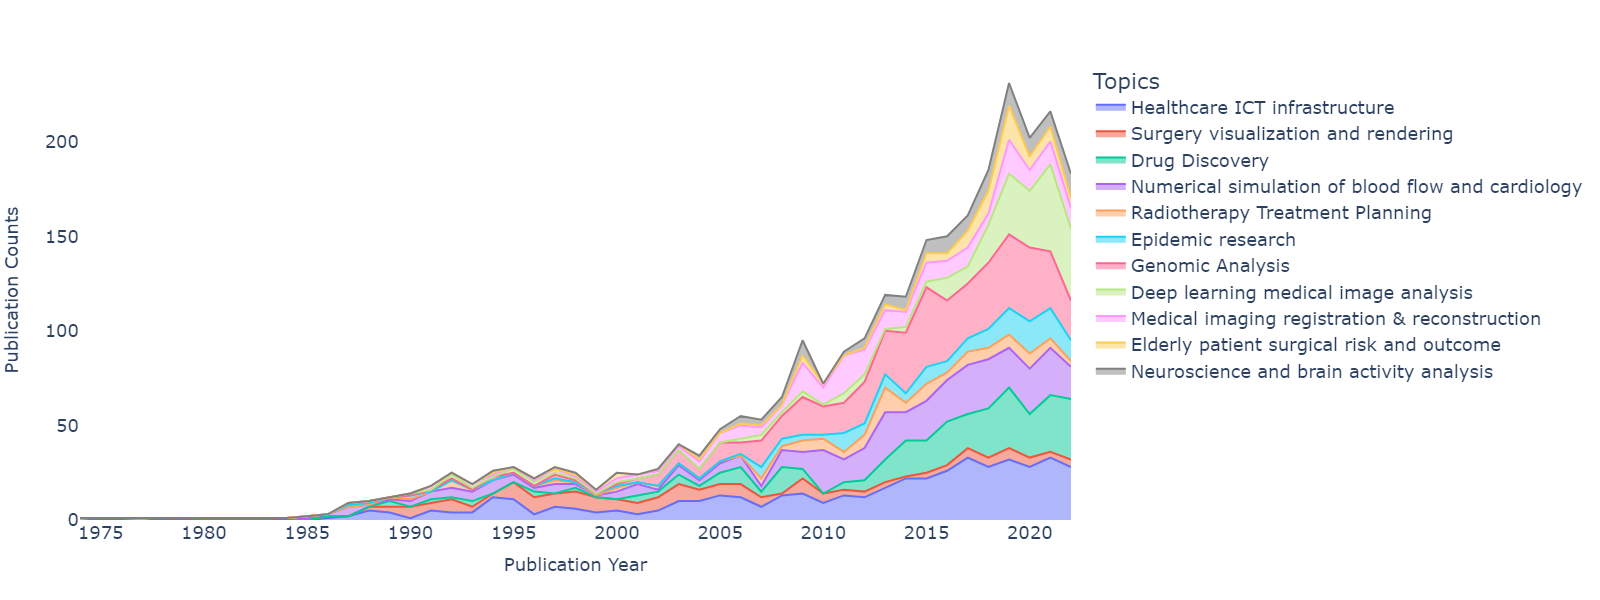
\includegraphics[width=1.0\textwidth]{2-4.png}
\caption{Stacked area chart illustrating trends in HPC adoption in healthcare cross application domains over time. Each segment represents a specific topic. The thickness of segments reflects topic-specific publication volume}
\label{fig:2-4}
\end{figure}

\begin{figure}[!h]
\centering
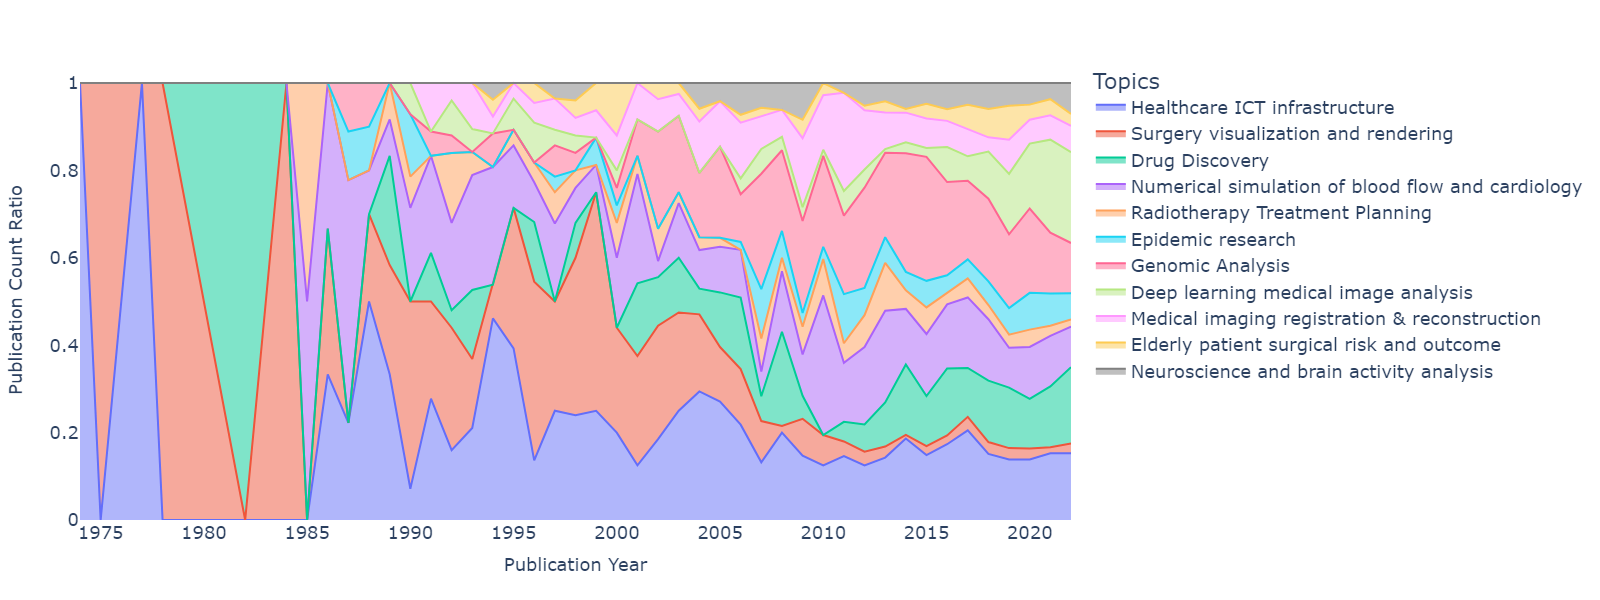
\includegraphics[width=1.0\textwidth]{2-5.png}
\caption{Normalized stacked area chart depicting the relative distribution of HPC adoption in healthcare across application domains over time. Each segment represents a specific topic. The thickness of segments reflects normalized proportion of publication counts}
\label{fig:2-5}
\end{figure}

The violin chart presented in Figure~\ref{fig:2-6} confirms the insights derived from the stacked area chart, specifically the extensive investigation of healthcare ICT infrastructure in the past thirty years. From 2005 onwards, a marked shift has been observed in the utilization of HPC in medical imaging research. Initially, the focus was predominantly on image registration and reconstruction. However, after 2015, there was a significant transition towards the incorporation of deep learning techniques for image analysis. Fluid dynamics simulations of blood flow and cardiology, which adopted HPC relatively early, witnessed a significant surge after 2008. Additionally, visualization and rendering in surgical practice, among the earliest applications of HPC, were hot research topics from 1990 to 2010, although interest has waned since. Moreover, research related to epidemic spreading emerged around 2003, concurrent with the SARS-CoV-1 outbreak in Asia, and experienced a tremendous increase in HPC utilization during the global spread of COVID-19, underscoring HPC's growing importance in managing global health crises. Another noteworthy observation is the rising popularity of research on risk and treatment outcomes for elderly patients since 2019, possibly correlated to pandemic research, given the heightened concern for elderly individuals during this crisis. Additionally, the exploding healthcare expenses and the increasing average age of the global population further underscore this emphasis.
\begin{figure}[!h]
\centering
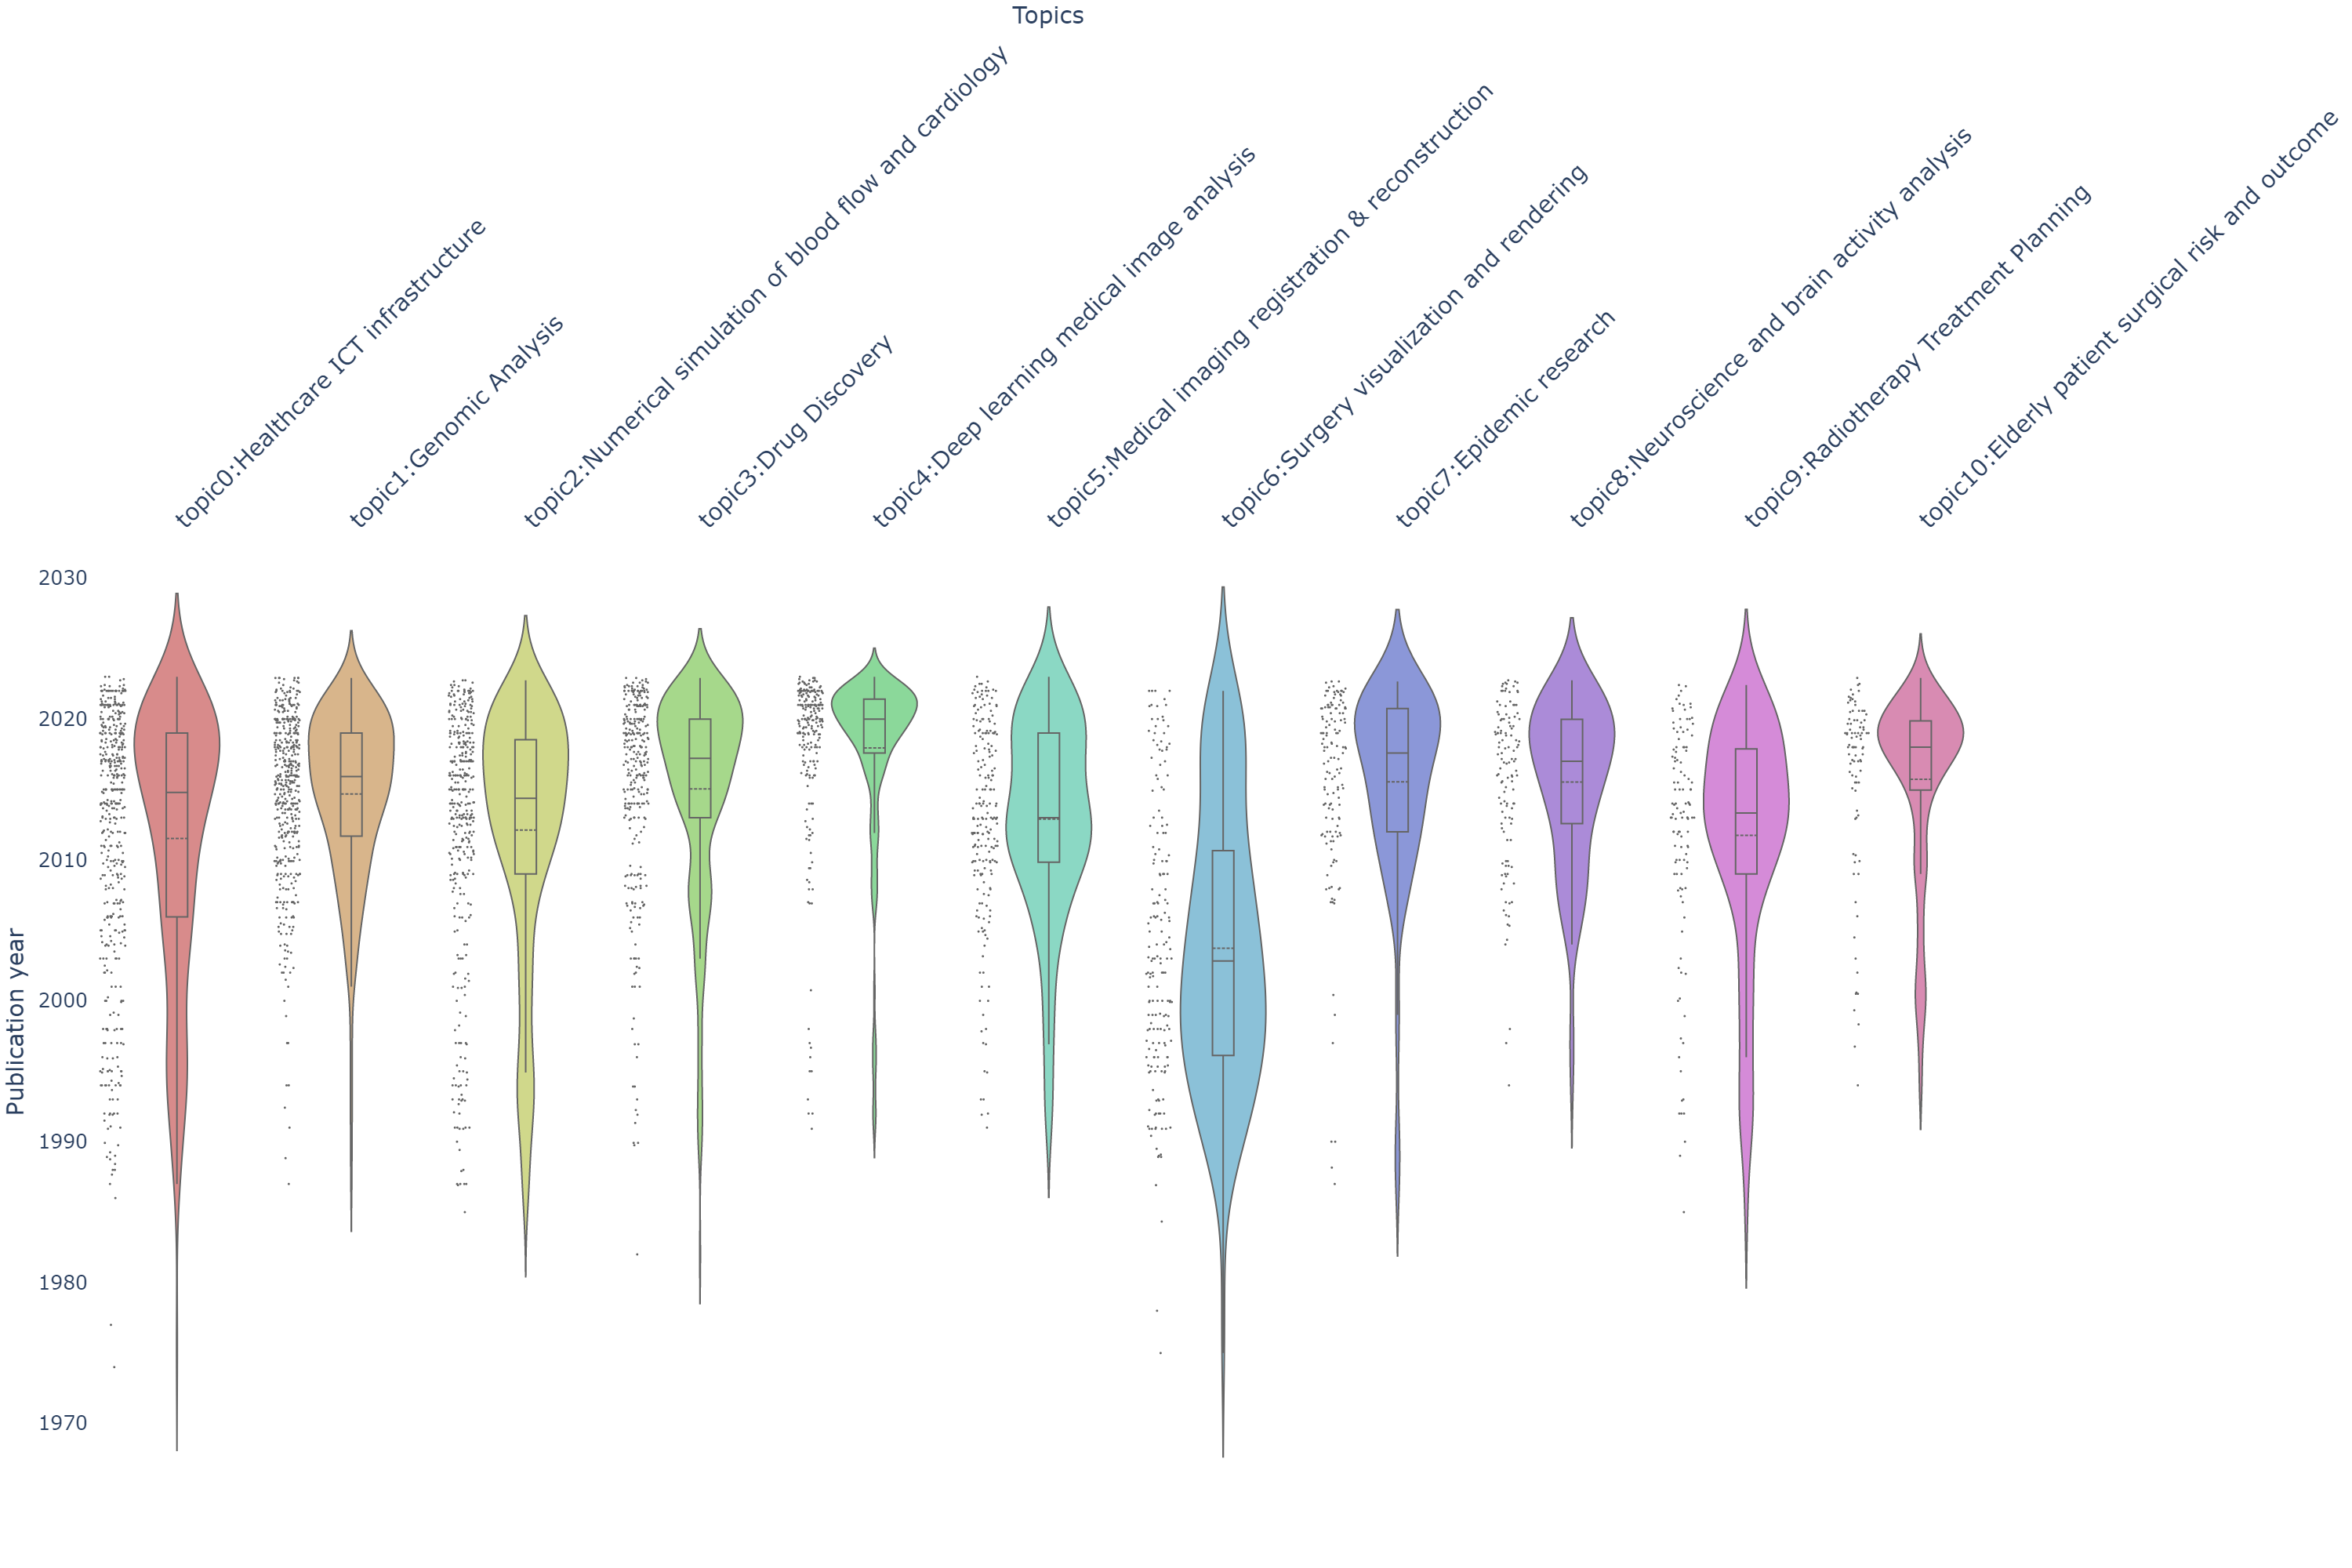
\includegraphics[width=1.0\textwidth]{2-6.png}
\caption{Violin chart depicting the distribution of HPC adoption in healthcare across application domains over time. Violin width represents publication density}
\label{fig:2-6}
\end{figure}

\subsection{Visualizations of topics correlation and convergence}\label{subse:2-3.4}

A bubble chart is constructed using UMAP to visually represent the coverage area of each topic (Figure~\ref{fig:2-7}). Translucent circles were utilized to depict the extent of coverage, while centroid topic vectors are indicated by triangular markers. Additionally, square markers are employed to symbolize the three most-cited papers for each topic. The top six keywords associated with each topic are also presented beneath their respective vectors. All publications form a point cloud, depicted in the background. The chart also incorporates interactive visualization mechanisms: hovering the mouse cursor over each square marker brings up details such as the paper's associated topics, ID, title, citation count, and abstract. This bubble chart provides substantial insights into the correlation and potential convergence trends of the topics, observable through the distances and overlaps between them. As indicated in Figure~\ref{fig:2-7}, a notable observation is the proximity of topics related to deep learning for medical image analysis to neuroscience and brain research. This suggests an extensive application of HPC-enabled medical imaging analysis within neuroscience research. In addition, the research related to simulations of cardiovascular \& blood flow, epidemic research, and drug discovery closely aligns with and overlap the topic of surgical risk and outcomes for elderly patients, indicating a focus on elderly patient outcomes across these topics. Furthermore, by examining the position of highly-cited papers within the bubble chart, we notice that some papers either represent pioneering studies, or span multiple domains, applying specific techniques to innovative fields. For instance, one of the highly cited papers titled `High performance computing for deformable image registration: Towards a new paradigm in adaptive radiotherapy'~\cite{samant2008high} (marked with a black arrow), is located in the intersection area of the topics `medical imaging registration \& reconstruction' and `radiation therapy planning'. This paper highlights the implementation of HPC for near real-time deformable image registration in radiotherapy, indicating that interdisciplinary papers might contribute to greater popularity and citation rates.

\begin{figure}[!h]
\centering
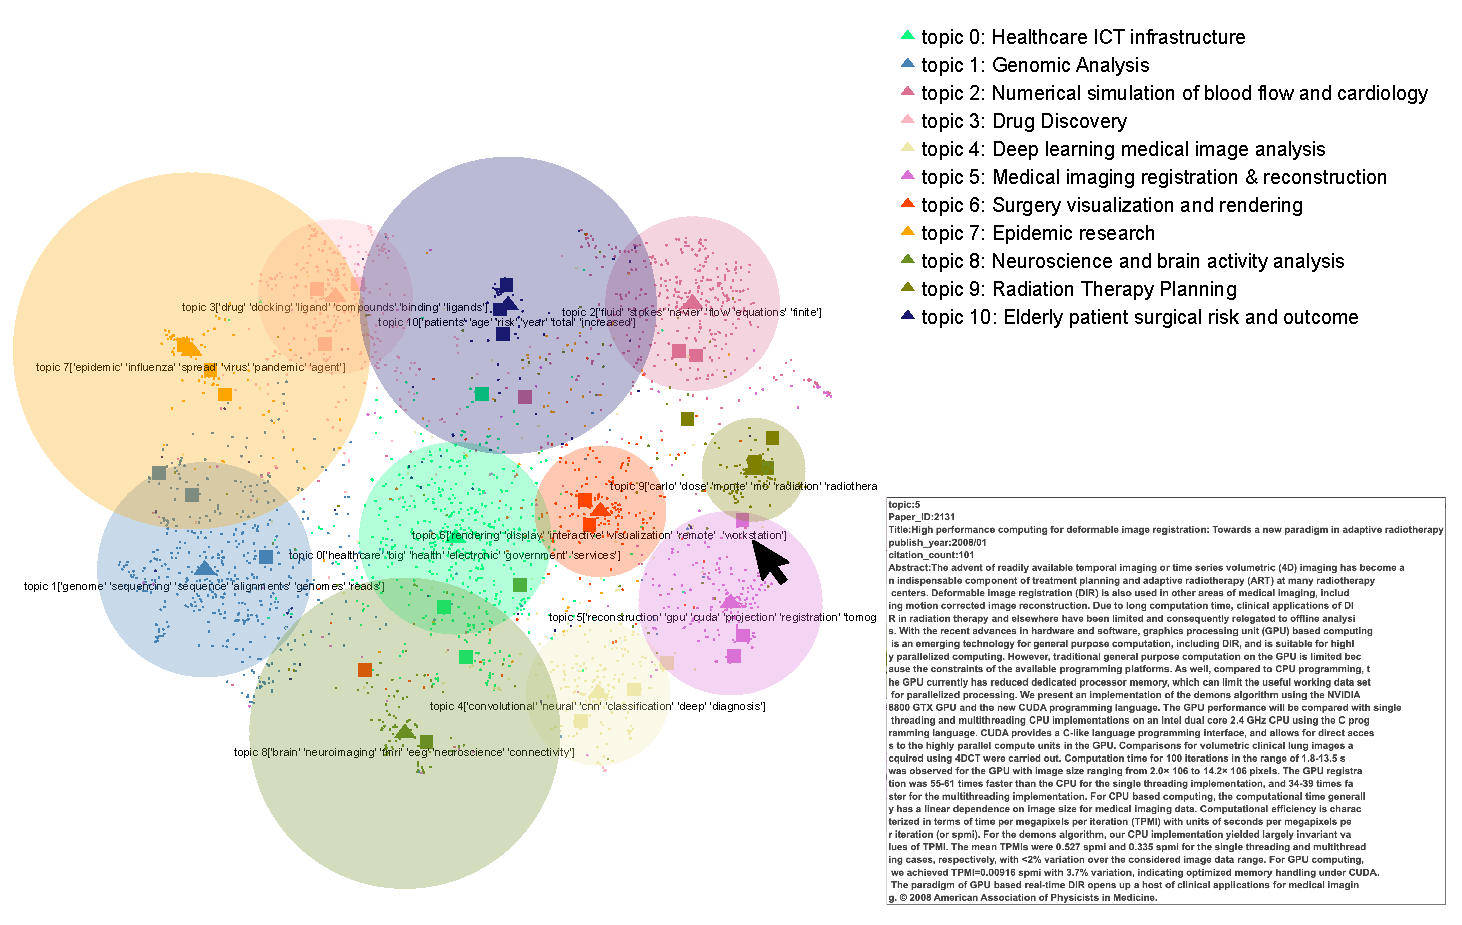
\includegraphics[width=1.0\textwidth]{2-7.pdf}
\caption{Bubble chart showing topic coverage areas based on UMAP. Translucent circles represent each topic's coverage area, centered at the topic's centroid and encompassing 70\% of associated literature. Centroid topic vectors are represented by triangular markers, and the three most-cited papers are indicated with square markers. A text box provides in-depth details on highly cited papers, including associated topics, ID, title, citation count, and abstract}
\label{fig:2-7}
\end{figure}

\section{Identifying future opportunities through analysis of past and present HPC adoption in healthcare}\label{se:2-4}

Historical analysis of HPC adoption within the healthcare sector illustrates a compelling transformation from a specialized technology  into a foundational tool for modern medicine. Originally, HPC was predominantly utilized for complex modeling and biological computations within academic research. However, its role has become more encompassing, opening new and fascinating medical and business opportunities over time. The convergence between simulation and AI, such as neural rendering, seamlessly melds computer graphics and deep learning, opening new avenues in diagnostics and personalized care. Concurrently, the consistent growth in genomics and drug discovery, accelerated by HPC, allows businesses to create dynamic models for pharmaceutical development, reducing cost and time-to-market. In addition, the rise of HPC in global epidemic research presents unique opportunities for developing real-time health monitoring systems, aligning commercial interests with public health needs, and enhancing our response to global health crises. The integration of HPC with emerging technologies such as AI and the Internet of Things (IoT) has further fostered innovative applications in telemedicine and remote monitoring, creating opportunities for healthcare providers to offer services across geographical boundaries. The fusion of technological advancements with unique patient needs has the potential to give birth to virtual care platforms, personalized treatment protocols, or even community-based wellness programs. These innovations align with the growing focus on aging populations, offering a compassionate and tailored approach to healthcare that could become a promising business domain.

The landscape of HPC adoption in healthcare represents an invitation to visionary business thinking, reflecting a future where innovation meets well-being. Collaboration among technology vendors, healthcare institutions, pharmaceutical companies, and startups can leverage the lessons learned from the past and the current state of HPC technology to forge partnerships, develop new products, and create service models that cater to an increasingly interconnected and data-driven healthcare environment. The analytical understanding of this evolution can serve as a guide for future endeavors, nurturing an ecosystem where technological advancement is aligned with healthcare requirements. In this convergence, both sectors stand to gain substantially from sustained cooperation and exploration. More importantly, as regulatory landscapes evolve to embrace technological advancement, it is imperative for stakeholders to understand the historical growth and current trends in HPC adoption in healthcare, as it will guide strategic decision-making and foster further innovation and growth in this interdisciplinary field. 

\section{Discussion}\label{se:2-5}

This study presents an automatic literature analysis framework that utilizes advanced topic modeling techniques (Top2Vec), within the context of the field of HPC adoption in healthcare as the testbed. Through this framework, we effectively process and analyze a substantial volume of scientific literature. The interactive visualizations shed light on the key trends and recognized the emerging research directions in a highly efficient manner. Given that the landscape of HPC adoption in healthcare is extensive and rapidly evolving, the automatic literature analysis offers a scalable and practical approach for researchers and stakeholders to identify trends and potential avenues for future exploration. Continuous tracking of these developments is necessary to maintain a dynamic understanding of the HPC landscape in healthcare, which enables the anticipation of its future.

One of the main limitations of using topic models, such as Top2Vec is the necessity for human intervention to determine the optimal number of topics, which is the only step requiring human input in our otherwise fully automatic literature analysis pipeline. Although metrics such as perplexity and coherence scores can provide guidance towards an optimal topic number, existing literature suggests that these metrics may occasionally be misleading and do not always align with human judgement~\cite{hasan2021normalized,harrando2021apples}. Determining the ideal number of topics within a topic model is a subjective decision that depends on the specific context and goals of the analysis. It requires a balance between having a sufficient number of topics to capture the underlying themes in the data and avoiding excessive fragmentation or overlap between topics. Therefore, human experience and judgment play a critical role in defining the optimal topic count. For this reason, we have integrated the use of a dendrogram to assist in determining the optimal topic count in a more intuitive manner.

Another challenge in using topic modeling is related to semantic understanding. While topic models are highly effective in identifying word and document patterns, they fundamentally lack the ability to understand the meaning of the words. This limitation can lead to topics that are difficult to interpret or exhibit semantic inconsistencies, making manual review and interpretation necessary. One possible approach to tackle this challenge is through EL, which can enhance topic modeling by providing an additional layer of explainability~\cite{dillan2023ldaviewer,10.1145/3126686.3126776}. By linking entities to a knowledge base, EL provides contextual understanding, which refines the interpretability of the topics. It effectively resolves ambiguities where identical names might refer to distinct entities, thereby improving the precision of topic clusters.  Moreover, while topic modeling can significantly aid in analyzing the vast volumes of scientific literature, it cannot replace the critical and contextual understanding that researchers bring to literature review. It should be regarded as a supplementary tool designed to assist in guiding literature exploration rather than serving as an autonomous solution. Given these limitations, future research should strive to fine-tune this methodology, improve the interpretability of the resulting topics, and investigate alternative methods for model evaluation. Despite the inherent challenges, topic modeling remains a potent instrument for managing and comprehending the ever-expanding corpus of scientific literature.

In conclusion, we propose an automatic literature analysis framework which can be easily applied across diverse literature domains, exemplifying its utility through the examination of literature within the field of HPC adoption in healthcare. The insights derived from this study are expected to guide researchers and practitioners toward recognizing emerging opportunities and challenges in the deployment of HPC in healthcare. These findings would contribute to a more informed and strategic incorporation of HPC in healthcare settings, holding the potential to transform medical research and clinical practice in the years to come.






















%!TEX root = ../dissertation.tex

\begin{savequote}[75mm]
Another inspiring quote for this chapter
\qauthor{Another author maybe}
\end{savequote}


\chapter[Improving the Speed and Quality of Cancer Segmentation Using Lower Resolution Pathology Images]{Improving the Speed and Quality of Cancer Segmentation Using Lower Resolution Pathology Images}
 
\lettrine[lines=3]{\textcolor{SchoolColor}{I}}{n this paper},
we propose a pipeline to investigate the performance of semantic segmentation model that employs an encoder-decoder architecture with atrous separable convolution and spatial pyramid pooling, trained on multi-resolution whole slide breast pathological images with different patch sizes. Our segmentation model obtains the best performance on zoom level 2 (10$\times$magnification) with AUC score 0.974 in terms of slide-level classification. This outperforms both the performance of the pathologist and other semantic segmentation models on the Camelyon16 dataset. By offering a larger field of view and reducing noise and detail, training
a semantic segmentation model on the properly selected lower resolution pathology images can further improve the precision of pixel-wise cancer region segmentation. By contrast, the corresponding inference time is 14 times shorter than the inference time trained on the highest resolution patches, and it is also shorter than the time required by a pathologist with time constraints.
Moreover, we prove that the model trained on lower resolution patches can still generate refined external polygons of cancer region on the highest resolution image. This study provides new insights into efficient gigapixel histopathology analysis that will make clinical adoption more likely.

\section{Introduction}\label{se:3-1}

As the highest incidence rate of cancer among women and the second leading cause of cancer death worldwide, breast cancer can be seen nowadays as the most serious threat to women's health. In 2019, 111,710 new cases of breast cancer were diagnosed worldwide and 41,760 woman died from it~\cite{Siegel2019}. However, with the development of pathology instrumentation and accessories, standardized pathological examination  can essentially contribute to better diagnosis and treatment of breast cancer. Especially in recent years, the possibility to capture an entire slide and save it in a digital format named Whole-Slide Image (WSI) enables pathologists to examine the biopsy at different levels of magnification, which significantly increased the accuracy of diagnosis~\cite{Pantanowitz2010}.  

However, manual microscope image examination is a time-consuming and tedious task and is made more difficult by the fact that tumor cells often occur as small patches that are difficult to spot. Computer-assisted pathology image analysis is therefore needed to help pathologists detect small metastatic areas in a more accurate and efficient manner. Machine learning has been widely adopted in the computer vision domain~\cite{khan2020machine,voulodimos2018deep,liu2020reliability}. For example, deep learning models and, particularly, Convolutional Neural Networks (CNNs), have been extensively utilized in medical image analysis~\cite{liu2021medical,liu2021review,Hou2016,Li2018,wang2021tumor,Deepa2022,gupta2022deep,singh2022breast,murtaza2020breast,chanchal2022deep}. In order to obtain better model accuracy, the number of parameters that need to be trained has dramatically increased, as CNN architectures go wider and deeper. However, training such models has significantly higher computation and memory demands. Hence, High Performance Computing (HPC) facilities based on CPU~\cite{codreanu2018}, GPU~\cite{Wang2022} and FPGA~\cite{Geng2018} enable training such heavy models while significantly reducing training times, which also benefits the WSI analysis.

The WSIs are typically high resolution images with a relatively large memory footprint. The size of one WSI could be around 2 gigabytes (GB) considering the slide image dimensions of 200,000 by 100,000 pixels in the highest resolution mode ($40\times$ magnification). However, since loading an entire WSI is currently still computationally intractable~\cite{Komura2018}, a typical approach to tackle this challenge is to extract smaller, manageable
patches from the highest resolution WSI and perform binary classification training and prediction of tumors by using deep convolutional neural network methods~\cite{Wang2016,Li2018}.

The Cancer Metastases in Lymph Nodes Challenge 2016 (i.e. CAMELYON16 or Camelyon16) was initiated by the IEEE International Symposium on Biomedical Imaging (ISBI) with the aim of detecting the presence of breast cancer metastases in lymph nodes~\cite{Bejnordi2017}. It has since become one of the most widely-used public datasets for studying cancer detection using deep learning methods~\cite{Wang2016,Liu2017,zhang2023whole,shen2022identify,yu2023bayesian,tourniaire2023ms,khaliliboroujeni2022end,jin2020integrative,liu2020effidiag,Guo2019}. The work presented in~\cite{Wang2016}, which won the Camelyon16 challenge~\cite{Bejnordi2017} with patches size $256\times256$ using GoogLeNet architecture~\cite{Szegedy2015}, reports the best results on the highest zoom level ($40\times$) images. However, this conclusion is based on patch-level classification, which has several limitations. Firstly, since the approach of patch level classification is predicting the whole patch as positive or negative, it ignores the situation where tumor and healthy tissue are coexisting in the same patch and can only generate prediction on very low resolution masks~\cite{Liu2017}. Secondly, in order to create relatively dense heatmap predictions, they have to extract relatively small patches such as $256\times256$ and $299\times299$ from the highest resolution ~\cite{Liu2017,Wang2016} . Such small patches on the highest resolution can not provide sufficient contextual information, which may lead to inconsistent predictions. Thus, there is a contradiction between patch size and dense prediction by using patch level classification methods. Some attempts have been made to consider the spatial correlations of neighboring patches such as introducing Conditional Random Field (CRF)~\cite{Li2018}. This has only been tested on small numbers of neighboring patches so the contextual information that can be learned is still limited. Finally, the number of patches extracted from single WSI would be around 10,000 to 400,000 (median 90,000)~\cite{Liu2017}, which is very time consuming and computationally intensive in terms of data preprocessing and prediction. 

In contrast, semantic segmentation models can generate refined predictions by performing pixel-level classification and do not need to consider the trade-off between patch size and prediction quality. In recent years, several attempts have been made to investigate the training of semantic segmentation models on the highest resolution WSI such as~\cite{Guo2019}. However, the performance of the model with the largest patch size $1024\times1024$ (AUC 0.95) reported from the paper is still lower than that of the pathologist without time constraints (AUC 0.966) with relatively long inference time (79~mins/slide) using one GTX 1080Ti GPU, which may hinder clinical adoption. Using similar-sized patches extracted from lower resolution WSI offers a larger field-of-view (FoV), since the amount of extracted patches for prediction is significantly smaller compared to the highest resolution one. This may contribute to better model performance and shorter inference time. Therefore, it is worth investigating the performance of semantic segmentation models on different zoom levels using HPC resources, as this facilitates pixel-wise classification instead of patch level classification.  

In this paper, we introduce a framework to evaluate the performance of a semantic segmentation model (DeepLabV3+) on various lower zoom levels, comparing them to the highest resolution patches ($40\times$ magnification), to explore the feasibility of training deep convolutional neural network with lower resolution images. We also conduct a comparison of model performance among different patch sizes trained on lower resolution. To our knowledge, no research has focused primarily on the trade-off between different zoom levels, segmentation models performance, and corresponding training and prediction time, which would offer insight into efficient gigapixel histopathology image analysis and its potential for clinical adoption.

The main contributions of this work are the following:

\begin{itemize}
\item Properly selecting lower resolution pathology images ($10\times$ magnification) can contribute to better semantic segmentation model training and prediction. It overcomes the limitation of patch-level classification using the highest resolution WSI, which generates low-resolution predictions by predicting the whole patch as positive or negative and ignoring coexisting tumor and healthy tissue within the same patch.
\item The semantic segmentation pipeline we proposed succeeds in outperforming pathologists. Additionally, the inference time is 14 times shorter than both the model trained on the highest resolution patches, and is also shorter than the time required by pathologists with time constraints.
\item Our model, trained on lower resolution patches ($10\times$ magnification), generates more precise segmentation than the same model trained on higher resolution patches. It accurately produces external boundaries of cancer regions on the highest resolution image ($40\times$ magnification), indicating its potential as a computer-assisted diagnostic and annotation tool to help pathologists reduce labeling time and identify cancerous regions.
\end{itemize}

\section{Dataset and evaluation metrics}\label{se:3-2}

To compare our workflow with state-of-the-art strategies, as a testbed for this study we adopt well-known Camelyon16 dataset, a publicly available WSI dataset of lymph node section~\cite{Bejnordi2017}. We further adopt the evaluation strategy from the Camelyon16 challenges with regard to  slide-level classification. The details are discussed in the following subsections.

\subsection{Camelyon16 dataset}\label{se:3-2.1}

The Camelyon16 dataset has 270 pixel-annotated WSIs obtained from the sentinel lymph nodes of breast cancer patients. The objective of the competition is to develop an algorithm capable of automatically detecting the scope of breast cancer metastasis in lymph node slices stained with Hematoxylin and Eosin (H\&E). These contain 110 metastases collected in the Radboud University Medical Center and the University Medical Center Utrecht. The average memory footprint of a WSI in the Camelyon16 dataset is around 1.9 GB, with the smallest WSI being 522MB and the largest 3.8GB. At the highest magnification level, WSIs have an average width of 109,666 pixels, ranging from 45,050 to 221,184 pixels, and an average height of 173,012 pixels, ranging from 28,672 to 221,696 pixels. The WSIs are stored in a 3-channel encoded TIFF format, which involves multiple levels of downsampling, to address the different zoom levels in one image. The largest resolution can be obtained at $40\times$ magnification, which is also considered level 0, while the magnification of $20\times$ corresponds to level 1, $10\times$ corresponds to level 2 etc.

\subsection{Evaluation metrics}\label{se:3-2.2}

In this study, we use the first evaluation strategy (i.e. Slide-based Evaluation) of the Camelyon16 challenge to measure the performance of our predictions\footnote[1]{https://camelyon16.grand-challenge.org/Evaluation/}. It enables us to compare our model results with the Public Leaderboard 1 in Camelyon16 challenge in terms of WSI classification task. This metric evaluates the performance of classification models at discriminating between WSIs which contain metastasis and normal slides. In the challenge, participants submit the list of probabilities which indicate the likelihood of each slide containing tumor and the area under the receiver operator curve (AUC) will be calculated to measure the performance of the model~\cite{Bradley1997}. We use percentile bootstrap method and construct 95\% confidence intervals for AUC score calculation~\cite{Efron1979}.

\section{Method}\label{se:3-3}

In this section, we further describe the testbed used for our study, including the complete proposed workflow, model details, and hardware configuration. Figure~\ref{fig:3-1} illustrates  the cancer metastasis detection workflow in our study, which can be divided into training and prediction pipelines. The training pipeline encompasses patch extraction from WSI tissue areas with multiple magnification levels and corresponding DeeplabV3+ model training. The prediction pipeline involves patch extraction, inference, pixel-wise tumor probability heatmap generation, cancer regions segmentation, and slide-based classification. The details are explained in the following subsections.

\begin{figure}[!ht]
\centering
\includegraphics[width=0.9\textwidth]{3-1.eps}
\caption{Overview of the proposed pipeline.}
\label{fig:3-1}
\end{figure}

\subsection{Data preprocessing}\label{se:3-3.1}

In this section, we describe how we removed the background area from the whole-slide images (WSI) to extract only the tissue area and generate non-overlapping patches. We also outline our data preparation and augmentation steps for model training. The details are discussed in the following subsections.

\subsubsection{Patch sampling}\label{se:3-3.1.1}

In our data preprocessing pipeline, we use Openslide~\cite{GOODE201327}, a C library that provides a simple interface for reading whole-slide images, to open the Camelyon16 pathology image files. To prevent generating many white (empty) patches, similar to~\cite{khened2021generalized} and inspired by Otsu's seminal work~\cite{4310076}, we convert WSIs from BGR to HSV color-space and threshold the three channels of HSV image in the range of 0 to 200 to obtain the tissue area,  We then perform morphological open and closing operations to eliminate any noise present. Next, we use the \texttt{cv2.findContours} and \texttt{cv2.boundingRect} functions to generate contours of the areas containing cell tissues and to draw a bounding box outside the contours in preparation for the patch extraction process. Subsequently, we extract non-overlapping patches of size ($768\times768$) using sliding windows inside the bounding boxes of these contours only. After generating a patch, a post-processing step is performed looking at the standard deviation of the patch in combination with the amount of black and white pixels, to investigate whether pixels in the patch are part of the artefacts in the background (e.g. some WSI's have black background). If that is the case, the patch is discarded. Using the same method, we extract the tissue area, calculate the percentage of tissue in each patch, and conduct the sampling as follows. For negative patch sampling, i.e. sampling of patches that do not contain any cancerous tissue, we only extract negative patches from normal WSI to avoid the interference of rough annotation. In addition, we select patches which contain more than 5\% tissue area. As for positive patch sampling, patches containing more than 0.5\% cancer area from tumor WSI are considered as positive patches. The ratio of positive and negative patches used for training is 1:3, which is different from some related work, such as~\cite{Lee2018,Li2018}, that sample the same number of tumor and normal patches. The reason for increasing the ratio of negative patches in the training set is the following: unlike patch-level classification, semantic segmentation models enable more precise prediction but also significantly increase the chance of wrong predictions, and in particular false positives, since they perform pixel level classification. Such wrong predictions will highly impact the WSI classification results. Contrary to balancing the classes by performing under-sampling of the majority category as in~\cite{Lee2018,Li2018}, we conjecture that a higher ratio of negative patches will allow the model to better capture variety in the data by avoiding loss of potentially useful information. We confirm this assumption empirically by obtaining a higher WSI classification accuracy when training the model with ratio 1:3 instead of 1:1.

\subsubsection{Patch augmentation}\label{se:3-3.1.2}

Since the slides of Camelyon16 are collected from two medical centers, staining variability is often present in the training dataset, which may be caused by different product of hematoxylin and eosin-stains or subtle difference in chemical staining procedures. Several publications indicate high staining variations will negatively affect the model performance~\cite{Lee2018,Dimitriou2019}. In general, there are two approaches to tackle this problem. The first approach is to implement stain-color normalization~\cite{Magee2009,Zanjani2018}. The second approach is to force the model to ignore the color variation in patches by adopting hard color augmentation~\cite{xu2020colorectal,wu2022machine}. 
In order to force the model to ignore staining variability, we adopt hard data augmentation due to the time-consuming nature of stain color normalization, which needs to be implemented during both the training and inference processes. We apply random hue, saturation, brightness and contrast as described in Table~\ref{tab:3-1}. In addition, we also add random flip to our data augmentation process.

\begin{table}[!h]
\centering
\caption{Patch augmentation details.}
\label{tab:3-1}
\setlength{\tabcolsep}{1.8mm}{
\begin{tabular}{lll}
\toprule
\textbf{Methods} & \textbf{Details} & \textbf{Triggering Probability} \\ 
\midrule
Random Hue & maximum delta of 0.2 & 0.66 \\
Random Saturation & random saturation factor in [0.5, 1.5] & 0.66 \\
Random Brightness & maximum delta of 0.5 & 0.66 \\
Random Contrast & random contrast factor in [0.7, 1.3] & 0.66 \\
Flip & Left/right flip & 0.66 \\ 
\bottomrule
\end{tabular}}
\end{table}

\subsection{Semantic segmentation model}\label{se:3-3.2}

For the semantic segmentation task we use the DeeplabV3+ architecture developed by Google~\cite{Chen2018}, which proved to be highly effective in semantic segmentation tasks on the benchmark datasets, such as PASCAL VOC 2012~\cite{Everingham2015} and Cityscapes~\cite{Cordts2016}. DeeplabV3+ architecture is shown in Figure~\ref{fig:3-2}.The whole network can be considered as an Encoder-Decoder structure. For the encoder part, it mainly uses the architecture proposed in the DeeplabV3 paper~\cite{Chen2017}, which includes dilated convolutional operators and Atrous Spatial Pyramid Pooling (ASPP) capable of extracting features at different scales of receptive fields. To ensure that the memory footprint of the activation maps and therefore model remains within the hardware boundaries, this scaling is done by dilating convolutional operators. The multi-scale traits of the architecture fit the hypothesis about achieving better tumor segmentation by enlarging the patch size, thus taking in account more information due to the larger scale. The formal definition of the atrous convolution operation on the input feature map $x$ is given in Equation~\eqref{eq:multiscale}. Here $f_{i}$ is the output feature map $f$ at location $i$, $\mathbf{c}$ is the convolutional filter with length $\ell$ and the dilation rate $d$ determines the stride of the input $\mathbf{x}$~\cite{Chen2018}.

\begin{figure}[!ht]
\centering
\includegraphics[width=1.0\textwidth]{3-2.eps}
\caption{An overview of DeeplabV3+ architecture.}
\label{fig:3-2}
\end{figure}

The decoder part is for the first time introduced in DeeplabV3+ architecture. In the former generation of Deeplab model (DeeplabV3)~\cite{Chen2017}, the encoder generates the feature maps with output stride 16, bilinearly upsampled to the original patch size. However, this method is not effective in terms of obtaining detailed object boundaries. Therefore, the decoder first upsamples the feature map generated from the encoder by a factor of 4. It then concatenates this with the low-level features from the backbone with corresponding spatial resolution after $1 \times 1$ convolution. Subsequently, the merged feature map will be passed through another $3 \times 3$ convolution and upsampled again by a factor of 4 to the original input size.
\begin{equation}
f_{i}=\sum_{\ell=1}^{\ell} \mathbf{x}(i+d \cdot \ell) \mathbf{c}(\ell)
\label{eq:multiscale}
\end{equation}

In addition, DeeplabV3+ uses atrous separable convolution to reduce the computation complexity of the proposed model while maintaining similar (or better) performance. It performs atrous convolution operations on each channel of input features separately, followed by a pointwise convolution to combine the output from atrous depthwise convolutions across channels. In our training process, we loaded the pre-trained PASCAL-VOC 2012 weights on the Xception backbone~\cite{8099678}. The Xception backbone in DeeplabV3+ has been modified as follows: (1) More layers are added. (2) All max pooling layers have been replaced with depthwise separable convolutions with strides. (3) Batch normalization and ReLU activation were introduced after each $3 \times 3$ depthwise separable convolution.

\subsection{Pipeline of WSI prediction}\label{se:3-3.3}

In order to evaluate the performance of our model trained on multiple zoom levels and patch sizes, we set up the WSI prediction pipeline, which is also illustrated in the testing stage of Figure~\ref{fig:3-1}. Similar to patch sampling, non-overlapping patches from different zoom levels are sequentially extracted from the bounding boxes of tissue area and fed into the trained model for inference. For example, $768\times768$ patches extracted from level 1 are sent to model trained on level 1 and so on. In order to accelerate the inference process, for level 0 and 1, we predict the patches which contain more than 20\% tissue area in order to avoid irrelevant predictions on background or fat tissue. As for level 2 and level 4, since the extracted patches have a relatively large field of view (FoV), we reduce the threshold of tissue area from 20\% to 10\% in order to avoid missing tissue area during the patch prediction. Figure~\ref{fig:3-3} shows an example of $768\times768$ patches extracted from the test set from level 0 to 4. Note that the extracted patches cover the tissue area of WSI. Similar to \cite{Li2018}, the patch prediction will be resized to the corresponding size on level 6 and stitched on a level 6 blank mask for post-processing. Since semantic segmentation inevitably leads to false positives, we first list the top 50 pixels from the WSI prediction based on the metastasis probability in descending order. Then, the mean of tumor probabilities is calculated and used as the likelihood of containing cancer for a single WSI.

\begin{figure}[!h]
\centering
\includegraphics[width=0.7\textwidth]{3-3.eps}
\caption{Patches extracted for prediction from different zoom levels}
\label{fig:3-3}
\end{figure}

\subsection{Hardware configuration}\label{se:3-3.4}

The training exercise of this study was implemented on the GPU nodes from the LISA Compute Cluster at the Dutch National Supercomputing Centre SURFsara\footnote[2]{https://userinfo.surfsara.nl/systems/lisa/description}. The training with patch sizes from 384 to 1024 on each level is performed on two GPU nodes, each consisting of one Intel Xeon Gold 5118 Processor and four NVIDIA Titan RTX GPUs with 24 GB of GDDR6 memory. For the inference step, we still used NVIDIA Titan RTX GPU node but only one GPU was needed for prediction because the inference process is not very time consuming. Therefore, the figures of prediction time presented in Table~\ref{tab:3-3} are based on using a single NVIDIA Titan RTX GPU.

\section{Results}\label{se:3-4}

We conduct a series of experiments to answer the following research questions:
\begin{enumerate}
\item How does the model performance change when training with multi resolution pathology images? Is it possible to achieve even a better result at lower magnification levels?
\item Can such training protocol on WSIs yield a comparable performance to pathologist and state-of-the-art automatic approaches working with high-resolution images?
\item What is the difference in inference time between models trained on different WSI resolutions and pathologist performance?
\item Can the presented model trained with lower resolution images still generate refined external polygons of cancer region on the highest resolution?
\end{enumerate}

\subsection{Performance of the model trained on different zoom levels and patch sizes}\label{se:3-4.1}

The results of our model trained on different zoom levels and patch sizes performing the Camelyon16 WSI Classification task are shown in Figure \ref{fig:3-4}. The left part of the figure presents the ROC curves of DeeplabV3+ trained from zoom level 0 to 4 with same patch size $768\times768$. AUC indicates the area under the receiver operating characteristic curve. We observe that the model trained on level 2 patches achieves the best AUC score of 0.9713. The figure on the right demonstrates the classification performance of models trained with four different patch sizes (i.e. 384, 512, 768, and 1024) on level 2. The model trained on $1024\times1024$ patch size achieves the best result (0.9741), and we observed a general trend suggesting that larger patches lead to better model performance. In addition, interesting comparison between the model trained with $384\times384$ patches on level 2 and $768\times768$ patches on level 1 can be made because they contain the same FoV. The result shows that the model trained with $384\times384$ patches on level 2 achieves better results (0.9591) than $768\times768$ patches on level 1 (0.9564), which indicates that even in the condition of same FoV, the model trained on level 2 still gets better performance. 

\begin{figure}[!h]
\centering
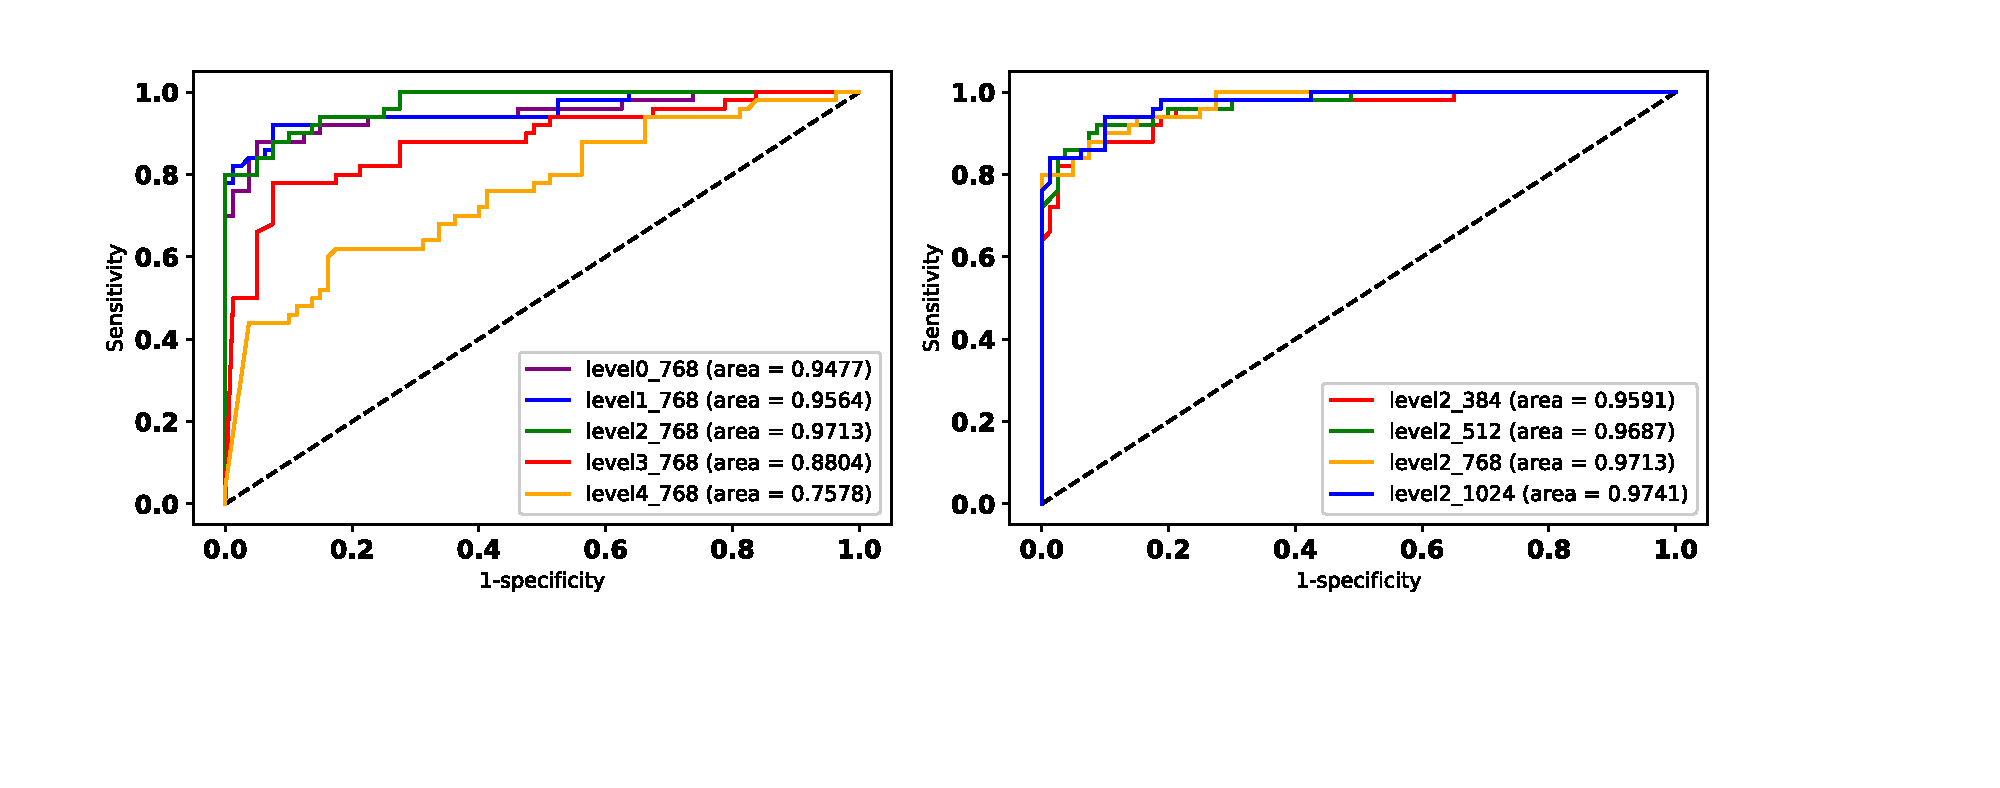
\includegraphics[width=0.95\textwidth,trim = 10 70 10 20, clip]{3-4.eps}
\caption{Comparison results of our models trained on different zoom levels
and patch sizes}
\label{fig:3-4}
\end{figure}

Figure \ref{fig:3-5} illustrates the comparison between our model trained on multiple zoom levels with a patch size of $768\times768$ pixels and the performance of pathologists, both without time constraints (WOTC) and with time constraints (WTC)~\cite{Bejnordi2017}. It firstly shows a clear trend on how model performance changes with the increasing zoom levels. Namely, the model performance improves in the WSI classification task when the zoom level increases from 0 to 2, but dramatically drops at levels 3 and 4. We assume that the reason for lower performance on zoom levels 3 and 4 lies in excessive down-sampling loses, which make it for the segmentation models very hard to distinguish tumor area from normal tissue. In addition, our model trained on zoom level 2 achieves better results than the pathologist WOTC.
\begin{figure}[!h]
\centering
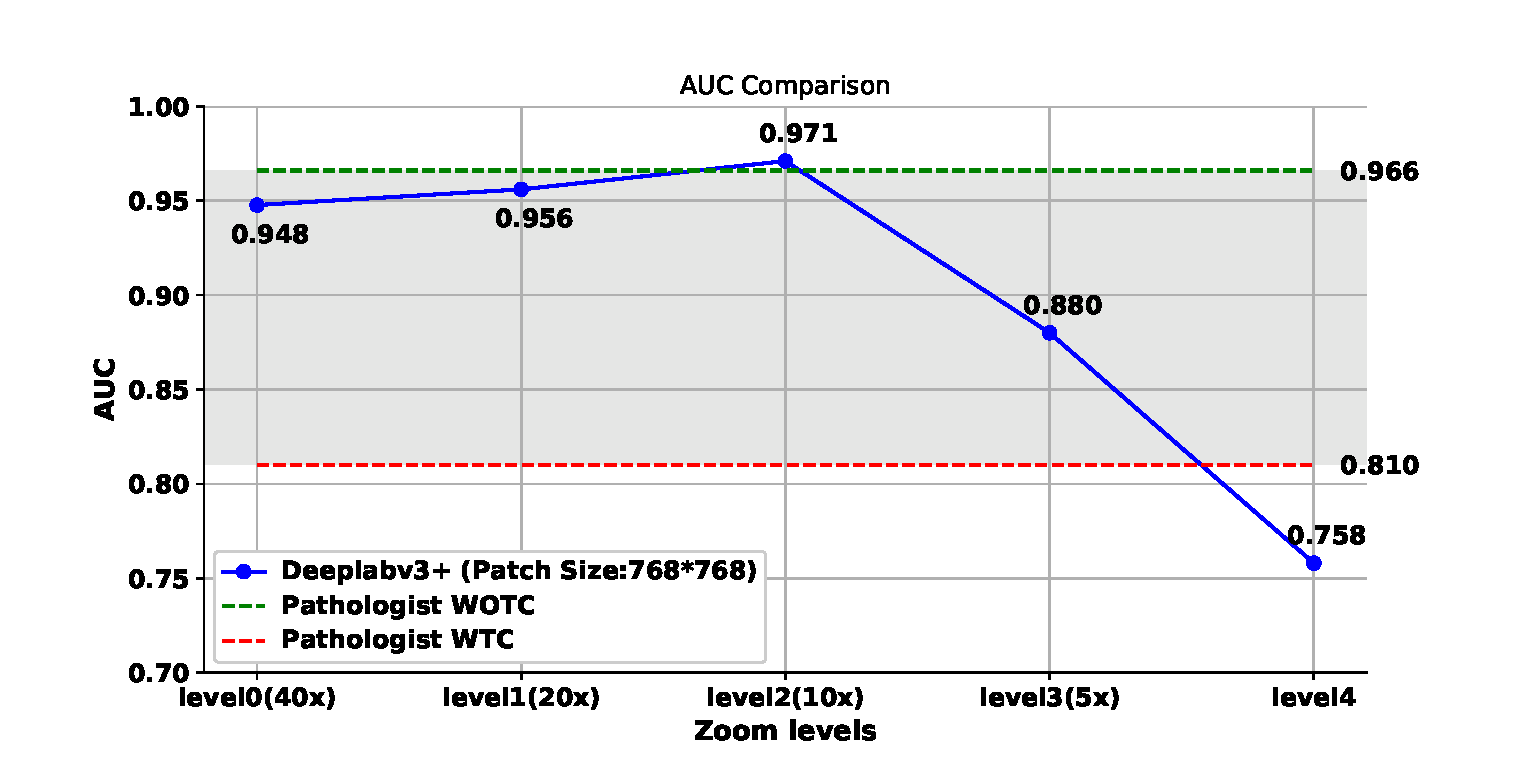
\includegraphics[width=0.9\textwidth]{3-5.eps}
\caption{Comparison results of our methods with pathologist performance}
\label{fig:3-5}
\end{figure}

\subsection{Comparison with state-of-the-art}\label{se:3-4.2}

In addition, we compared our results with the official leaderboard of the Camelyon16 challenge and state-of-the-art papers using Camelyon16 dataset (Table \ref{tab:3-2}). Our pipeline based on DeeplabV3+ model trained with $1024\times1024$ patches on level 2, achieved third place in Whole-slide-image classification public Leaderboard 1 \cite{camelyon16}. It should be noted that a remarkable AUC score of 0.994 can be achieved by employing additional computationally demanding procedures, such as stain normalization and a smaller inference stride. However, this outcome is less noteworthy and presents considerable obstacles to clinical implementation due to the substantially increased computational expense. Ideally, the diagnostic process should be executed promptly with minimal resource utilization. Since 2019, several papers studied the performance of more recent segmentation models on Camelyon16 dataset. The study presented in \cite{jin2020integrative} used ConcatNet (Four U-nets based on four histological features) and achieved an overall AUC 0.924. Another study \cite{Liu2017} applied Unet and EffiNet, yielding an overall AUC of 0.935. The research presented in \cite{Guo2019} implemented a classification model Inception-v3, followed by the use of a semantic segmentation model DCNN for enhanced segmentation, leading to an overall AUC of 0.966. However, those results didn't exceed the pathologist performance WOTC. Our model trained on level 2 patches obtained the best result (AUC 0.9742) for semantic segmentation on Camelyon16 dataset in terms of WSI classification task. 

\begin{table}[!h]
\centering
\caption{Comparison of the results obtained by our model trained on different zoom levels and state-of-the-art methods; we make a distinction between patch level classification and semantic segmentation prediction approaches}
\label{tab1}
\label{tab:3-2}
\setlength{\tabcolsep}{0.8mm}{
\begin{tabular}{p{3cm}p{4.8cm}p{3.67cm}p{0.9cm}}
\toprule
Author & Method & Prediction method & AUC \\
\midrule
Pathologist~\cite{Bejnordi2017} & N/A& N/A & 0.966 \\ 
Wang et al.~\cite{Wang2016}  & GoogLeNet& Patch level classification& \textbf{0.994} \\ 
Liu et al.~\cite{Liu2017} & ResNet & Patch level classification& 0.976\\
Zhang et al.~\cite{zhang2023whole} & DPN, Swin-Transformer, SVM & Patch level classification& 0.961\\
\multirow{2}*{Shen et al.~\cite{shen2022identify}} & Pathology Deformable Conditional Random Field & \multirow{2}*{Patch level classification} & \multirow{2}*{0.920}\\ 
Yu et al.~\cite{yu2023bayesian}  & Bayesian
Collaborative Learning & Patch level classification & 0.956\\
Tourniaire~et~al. \cite{tourniaire2023ms} & Mixedly Supervised-CLAM & Patch level classification & 0.982\\
Khaliliboroujeni et~al.~\cite{khaliliboroujeni2022end}  & ResNet50, spatial 
 and channel attentions & \multirow{2}*{Patch level classification} & \multirow{2}*{0.970}\\
\midrule
Quincy Wong~\cite{Bejnordi2017}  & SegNet & Semantic Segmentation & 0.865  \\ 
Jin et al.~\cite{jin2020integrative} & ConcatNet & Semantic Segmentation & 0.924 \\ 
\multirow{2}*{Liu et al.~\cite{liu2020effidiag}}  & \multirow{2}*{Unet, EffiNet} & Semantic Segmentation\! + Patch level classification & \multirow{2}*{0.935}\\
\multirow{2}*{Guo et al.~\cite{Guo2019}}  & \multirow{2}*{v3\_DCNN\_1280 (level0)} & Patch level classification +\!\!~Semantic Segmentation & \multirow{2}*{0.966}\\  
Our method& DeeplabV3+\_1024\! (level2) & Semantic Segmentation & \textbf{0.974} \\ 
Our method& DeeplabV3+\_768 (level2) & Semantic Segmentation & 0.971\\ 
Our method& DeeplabV3+\_512 (level2) & Semantic Segmentation & 0.969\\
\bottomrule
\end{tabular}}
\end{table}

\subsection{Training and prediction time comparison}\label{se:3-4.3}

Next to prediction accuracy, another important factor influencing clinical adoption is the average inference time on a single WSI. We only use one NVIDIA Titan RTX GPU to perform inference. Table \ref{tab:3-3} shows the Training and inference time comparison among our models trained on multiple zoom levels and patch sizes. The model trained on level 2 with a patch size of $1024\times1024$ has the shortest inference time (42 s per slide), which is lower than that needed by a pathologist WTC (56 s per slide)~\cite{Bejnordi2017}. This is because the number of patches extracted from lower resolution WSI for prediction is much lower than in case of the highest resolution. Based on the experimental results above, we propose that zoom level 2 ($10\times$ magnification) would be the appropriate magnification level to perform semantic segmentation on.

\begin{table}[!h]
\centering
\caption{Training and prediction time comparison of our models trained on different zoom levels and patch sizes}
\label{tab:3-3}
\setlength{\tabcolsep}{0.9mm}{
\begin{tabular}{lp{0.11\textwidth}p{0.07\textwidth}lp{0.10\textwidth}p{0.12\textwidth}p{0.14\textwidth}}
\toprule
Zoom level & Training set size & Batch size & Iterations & Training (h) & Prediction (h) & Prediction/ slide (m) \\ 
\midrule
{level 0($768\times768$)} & {56,632}& {4}& {25,000}& {10.12}& {21.31} & 9.83 \\
{level 1($768\times768$)} & {34,524}& {4}& {25,000}& {9.72} & {4.75}& 2.19 \\ 
\midrule
{level 2($1024\times1024$)} & {8,494}& {2}& {50,000}& {28.42} & {1.52}& {\textbf{0.70}}\\
{level 2($768\times768$)} & {10,420}& {4}& {25,000}& {9.58} & {1.55}& 0.71\\
{level 2($512\times512$)} & {23,256}& {4}& {25,000}& {6.2}& {2.12}& 0.97 \\
{level 2($384\times384$)} & {37,688}& {4}& {25,000}& {4.92} & {3.1} & 1.43 \\ 
\midrule
{level 3($768\times768$)} & {4,184} & {4}& {25,000}& {9.96} & {0.58}& 0.26 \\
{level 4($768\times768$)} & {1,992} & {4}& {25,000}& {9.23} & {0.23}& 0.18 \\ 
\bottomrule
 & & & & &&\\ 
\cmidrule{1-4}
\multicolumn{4}{l}{Pathologist WOTC: 13.95 m/slide}&&& 
\\
\multicolumn{4}{l}{Pathologist WTC: 0.93 m/slide} &&& \\ 
\cmidrule{1-4}
\end{tabular}}
\end{table}

\subsection{Segmentation result presentation}\label{se:3-4.4}

As we described previously, one of many advantages of performing semantic segmentation compared with patch-level classification is that it can offer refined cancer regions segmentation on high resolution WSIs, which can assist pathologists in identifying small metastasis area. This method could also be very useful when considered as a computer-aided annotation tool, which can significantly reduce the time of annotation for a pathologist. Therefore, it is worth evaluating the real segmentation performance of our model on both higher and lower resolution patches. In this study, we select our model trained on level 2 with a patch size of $768\times768$, as well as a model trained on level 1 with the same patch size, to generate binary predictions from heatmaps using a threshold of 0.5. Subsequently, we use \texttt{cv2.drawContours} function from OpenCV\footnote[3]{https://opencv-python-tutroals.readthedocs.io/} library to draw external polygons of cancer area. The segmentation result is shown in Figure \ref{fig:3-6}. Both models trained on level 1 and 2 can generate decent external polygons of the cancer area. However, we observe that the model trained on level 2 performs more precise segmentation than the one trained on level 1. The yellow arrows in Figure \ref{fig:3-6} show that some  subtle normal tissue and blank areas between tumor areas have been detected by the level 2 model but not by the level 1 one. In addition, several publications have discussed the issue of inaccurate labeling in histopathological imaging, including the Camelyon16 dataset~\cite{cheng2020self,gildenblat2019self,naouar2023robust}. Manually annotating large whole slide images on the pixel level of the highest magnification is an inherently challenging task, making it difficult to avoid unreliable labeling in practice. Notably, our model has the ability to accurately identify and label these areas. The fourth row of Figure~\ref{fig:3-6} illustrates an example in which some adipocytes were mistakenly labeled as tumors in the original mask, but our model trained on level 2 patches was able to accurately identify and correct them. Moreover, column (d) of Figure~\ref{fig:3-6} shows that even at the highest resolution, the polygons generated by our model trained on level 2 can still fit well with the tumor boundary, which indicates the interesting potential of our method in assisting pathologists with annotating high resolution images.

\begin{figure}[!h]
\centering
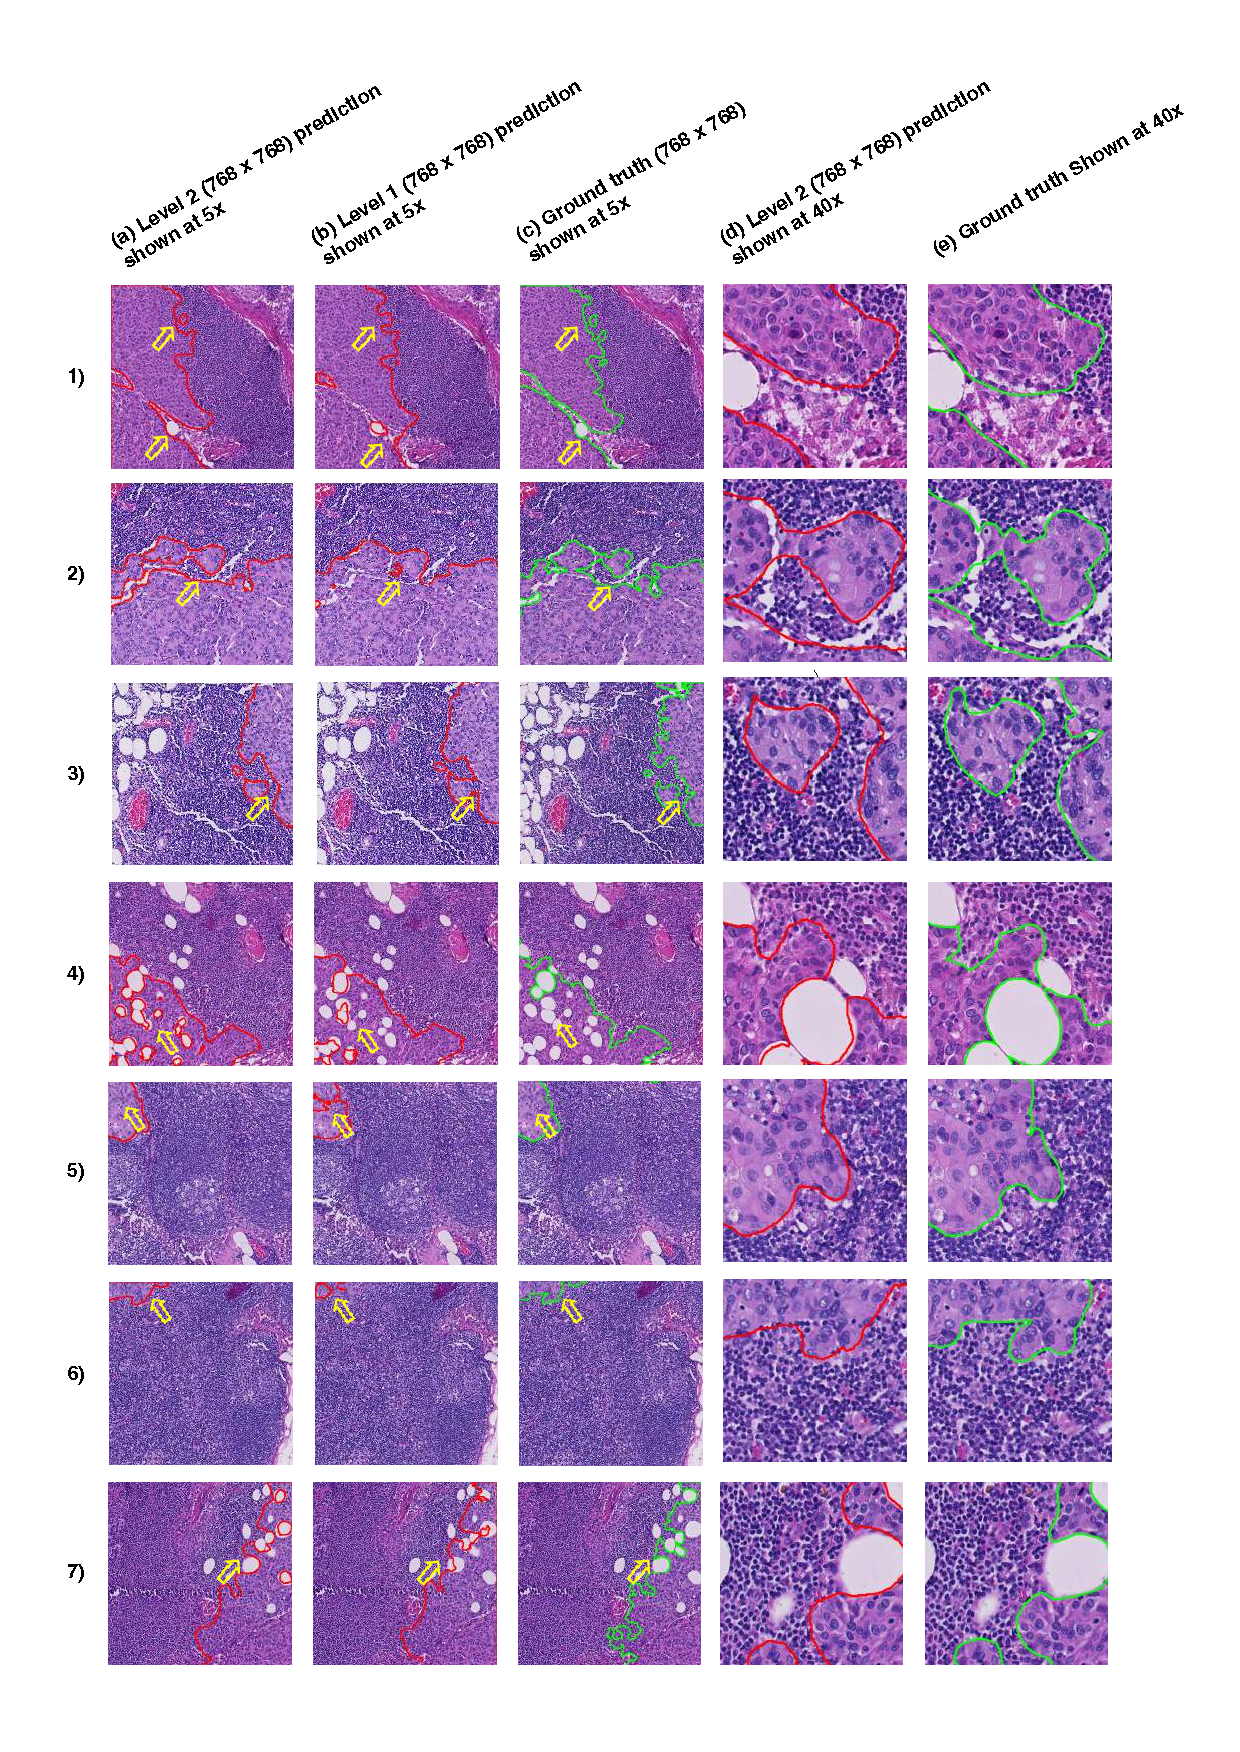
\includegraphics[width=0.9\textwidth]{3-6.eps}
\caption{External polygons of tumor regions generated by our models. From left to right, (a) is the prediction of model trained on level 2 shown at level 3 ($5\times$) patches, (b) is the prediction of model trained on level 1 shown at level 3 ($5\times$) patches, (c) is the Ground truth shown at level 3 ($5\times$), (d) is the prediction of model trained on level 2 shown at level 0 ($40\times$) patches, (e) is the ground truth shown at level 0 ($40\times$) patches.} 
\label{fig:3-6}
\end{figure}

We conjecture that the reason why the model on level 2 obtains the best result could be two-fold. Firstly, similar-sized patches extracted from lower resolution WSI offer a larger field-of-view (FoV), which contributes to better model performance in terms of segmentation and slide-level classification~\cite{Guo2019}. Secondly, although semantic segmentation models highly rely on the quality of annotation when performing supervised learning, it is nearly impossible for the pathologist to annotate pixel by pixel on the high resolution image. Therefore, training segmentation model on the highest magnification level would enable the model to obtain more details of tissue but at the same time, rough annotations also have a strongly negative impact on the performance of the model. Appropriate downsampling can makes the rough annotation on the highest resolution not obvious, therefore increasing the robustness of the segmentation model. Similar effect can be observed in using Gaussian filter to smooth the image and reduce the level of noise, which trades for better segmentation model performance~\cite{cai2017framework,nasor2021segmentation}. 

\section{Conclusion}\label{se:3-5}

In this paper, we study the impact of adopted resolution level and patch size on the performance of cancer region segmentation based on whole-slide images (WSIs) of sentinel lymph node. Firstly, we observe that the model achieves the best performance in the WSI classification task on zoom level 2 under the condition of same patch size and same field-of-view. Such results indicate that zoom level 2 (10$\times$) constitutes an appropriate magnification level for training and prediction of the semantic segmentation model in cancer metastasis detection. This interesting finding shows the possibility of efficiently training deep convolutional neural networks with lower resolution images. Secondly, the model trained on zoom level 2 patches achieved better performance than pathologist WOTC and, at same time, lower inference time than the pathologist WTC, which may help potential clinical adoption. Conclusively, our model trained on zoom level 2 patches can perform more precise segmentation than the same model trained on the higher-resolution patches, while still being able to generate refined external polygons of cancer regions on the highest resolution image. It indicates the potential of using these techniques as the basis for computer-aided annotation tools that help pathologists reduce the time taken by labeling. Further research on WSI analysis could include training models on zoom level 2 with even larger patch sizes, which can possibly lead to the training based on the entire WSI using more HPC capacity. The study could help identify the patch size for which the model performance becomes saturated and also show the limitations of current HPC facilities in terms of memory capacity. Moreover, it would be also interesting to explore the effects of using both data-parallelism and model parallelism strategies to process even larger patch sizes with the same model and hardware constraints.

%!TEX root = ../dissertation.tex

\begin{savequote}[75mm]
Another inspiring quote for this chapter
\qauthor{Another author maybe}
\end{savequote}


\chapter[An early health technology assessment in the Netherlands]{Cost-Effectiveness Analysis of CT-Based Finite Element Modelling for Osteoporosis Screening in secondary fracture prevention: An early health technology assessment in the Netherlands}

\lettrine[lines=3]{\textcolor{SchoolColor}{{\bf O}}}{
{\bf bjective:} To conduct cost-utility analyses for Computed} Tomography To Strength (CT2S), a novel osteoporosis screening service, compared to dual-energy X-ray absorptiometry (DXA), Treat all without screening, and No Screening methods for Dutch postmenopausal women referred to fracture liaison service (FLS). CT2S employs CT scans to generate femur models and simulate sideways fall scenarios for bone strength assessment.

{\bf Methods:} Adopted early health technology assessment (HTA) to evaluate CT2S as a novel osteoporosis screening tool for secondary fracture prevention. We constructed a two-dimensional simulation model considering four strategies (No Screening, Treat all without screening, DXA, CT2S) together with screening intervals (5 years, 2 years), treatments (oral alendronate, zoledronic acid) and discount rate scenarios, among Dutch women in three age groups (60s, 70s, and 80s). Strategy comparisons were based on cost-effectiveness ratios (ICERs), considering an ICER below \texteuro 20,000 per QALY gained as cost-effective in the Netherlands.

{\bf Results:} Under the base case scenario, CT2S vs. DXA had estimated ICERs of \texteuro 41,200 and \texteuro 14,083 per QALY gained for 60s and 70s age groups, respectively. For the 80s age group, CT2S was more effective and less costly than DXA. Changing treatment from weekly oral alendronate to annual zoledronic acid substantially decreased CT2S vs. DXA ICERs across all age groups. Setting the screening interval to 2 years increased CT2S vs. DXA ICERs to \texteuro 100,333, \texteuro 55,571, and \texteuro 15,750 per QALY gained for the 60s, 70s, and 80s age groups, respectively. In all simulated populations and scenarios, CT2S was cost-effective (in some cases dominant) compared with Treat all strategy and cost-saving (more effective and less costly) compared to No Screening.

{\bf Conclusion:} CT2S was estimated to be potentially cost-effective in the 70s and 80s age groups considering the willingness-to-pay (WTP) threshold of the Netherlands. This early HTA suggests CT2S as a potential novel osteoporosis screening tool for secondary fracture prevention. 

\section{Highlights}
\begin{enumerate}
\item For post-menopausal Dutch women who have been referred to FLS, direct access to CT2S may be cost-effective compared to DXA for age groups 70s and 80s, when considering the ICER threshold of the Netherlands. This study positions CT2S as a potential novel osteoporosis screening tool for secondary fracture prevention in the clinical setting.
\item A shorter screening interval of two years increases the effectiveness of both screening strategies, but the ICER of CT2S compared to DXA also increased substantially which made CT2S no longer cost-effective for the 70s age group, but it remains cost-effective for the age group in their 80s.
\item Annual zoledronic acid treatment with better adherence may contribute to lower cost-effectiveness ratio when comparing CT2S to DXA screening and Treat all strategies for all age groups.
\end{enumerate}

\section{Introduction}

In the last decade, specialised fracture and osteoporosis clinics called fracture liaison service (FLS), run by nurse practitioners and supervised by physicians, have been introduced in several countries including the Netherlands \cite{4-1}. Typically, FLS employ dual-energy x-ray absorptiometry (DXA) screening for the persons with previous fracture history to measure the areal bone mineral density (aBMD) and then offer treatment advice, if necessary, to the referring practitioner \cite{4-1}. This radiological exam directly gives a measure of the bone mineral content, which is compared with epidemiological data in order to evaluate its deviation from the average healthy population. However, the predictive performance of DXA in terms of fracture risk prediction is not perfect \cite{4-2,4-3,4-4}, depending on the characteristics of the individual patient. For this reason, various authors have proposed an alternative measurement technique, called Biomechanical Computed Tomography analysis (BCT), also known as a digital twin, using a low-dose CT scan and a patient-specific computer-based biophysics model to predict the fracture force of the femur \cite{4-4,4-5,4-6}. Computed Tomography To Strength (CT2S) is a particular implementation of the BCT, developed in collaboration between the University of Sheffield (UOS) and the University of Bologna (UNIBO) \cite{4-3,4-6,4-7}. 

 CT2S is run as an online service (https://ct2s.insigneo.org/ct2s/) hosted at the University of Sheffield. The user (usually clinician) would make a job request via the website. The user then uploads anonymised patient CT scans through the website’s secure portal. The CT scans are downloaded by the CT2S operator. The femur shape is segmented in 3D and meshed using finite elements. The local material property of the femur is estimated based on the CT attenuation. This fully personalised model of the femur is then used to simulate various sideways fall scenarios including all feasible ranges of loading directions to determine the failure load of the bone (i.e. bone strength) and the weakest orientation. This information is then used to calculate the Absolute Risk of Fracture at present, or time 0 (ARF0), which is the ratio between the number of falls (that led to fracture) over the total number of falls. The results are then summarised in a simple PDF file, which is sent back to the user who requested the job \cite{4-8}.

Evaluation of the CT2S approach showed better discrimination between fractured and non-fractured groups in a pair-matched elderly cohort of 98 women, who are prone to osteoporosis. The area under the receiver operating characteristic curve (AUC) was 0.85 using CT2S compared with 0.75 using the aBMD-DXA as the predictor \cite{4-3,4-6,4-7}. This study was conducted in a single National Health Service (NHS) centre at Sheffield in the United Kingdom. Similar results have also been shown in studies conducted in other countries \cite{4-9}, using cohorts of different age, race and sex. It is worth mentioning that other groups have used BCT to also analyse vertebral fracture \cite{4-9}.  However, such analysis has not been done using CT2S. Nevertheless, the question remains as to whether the higher costs associated with measuring the CT2S biomarker would be expected to translate into meaningful health benefits and whether those benefits would be expected to be cost-effective in osteoporosis screening in the Netherlands.

According to the Health Insurance Act (Zorgverzekeringswet), all residents of the Netherlands are legally obliged to take out standard health insurance \cite{4-10}. The cost of examinations and medications prescribed by the general practitioner or medical specialist is covered by the standard health insurance (e.g. DXA screening) \cite{4-11}. Each year, the government updates the national healthcare scheme and the insurance companies are mandated to incorporate changes within their offered benefits. Health policy decision makers would be interested in acknowledging whether the novel osteoporosis screening tools are potentially cost-effective relative to DXA for particular populations in order to consider further development, investments, and reimbursement policies. 

Early health technology assessment (HTA) is a methodology employed to evaluate the potential value and feasibility of emerging innovations at their early stages \cite{4-12}. Therefore, early HTA is necessary for providing the initial insight by revealing the cost and health quality outcome of different osteoporosis screening strategies. In this study, we adopted early HTA to assess the potential value of CT2S to be used as a novel osteoporosis screening tool. We used a two-dimensional simulation to estimate data on which a cost-utility analysis (CUA) was conducted for four strategies: CT2S, the standard of care represented by aBMD (hereafter referred to as `DXA') \cite{4-13}, treat all patients without screening and no screening in postmenopausal women referred for assessment to the FLS.

\section{Methods}
\subsection{Study Perspective}

The following cost-effectiveness analysis was conducted from a healthcare system perspective, as it considered the costs and consequences incurred by the healthcare system.

\subsection{Screening Scenarios and Strategies}

The following scenarios were simulated: three age groups (60s, 70s and 80 years), two screening intervals (5 years as the base case and 2 years in scenario analysis), two types of treatment (weekly oral alendronate as the base case and once-yearly intravenous infusion of zoledronic acid in scenario analysis) and two discount rates (4.0\% and 1.5\% for costs and effectiveness as the base case according to the Dutch guideline for economic evaluations in healthcare \cite{4-14} and 3\% rate for benefits as well as costs in scenario analysis). Each scenario consists of a combination of age groups, screening intervals, treatments and discount rates, with four strategies: CT2S screening, DXA screening, Treat all and No Screening, (Fig. \ref{fig:4-1}).

\begin{figure}[!h]
\centering
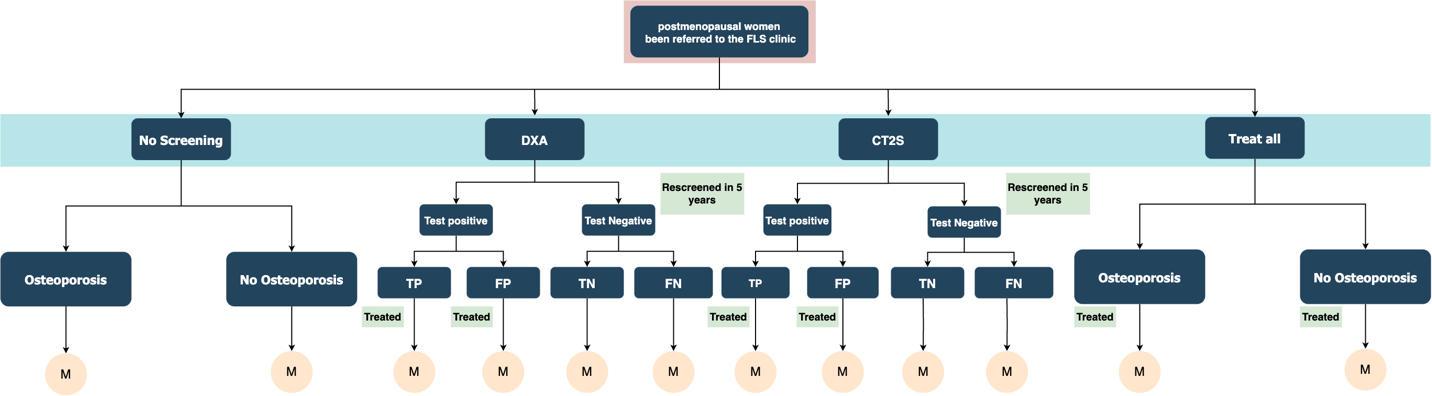
\includegraphics[width=1.0\textwidth]{4-1.png}
\caption{Diagram of screening model, TP = True Positive, FP = False Positive, TN = True Positive, FN = False Negative, M = Markov Chain.}
\label{fig:4-1}
\end{figure}

\subsection{Screening Interval}

In the literature, a variety of osteoporosis screening intervals have been suggested. An Australian clinical guideline for osteoporosis prevention and treatment suggests that follow-up screening should not be scheduled fewer than 2 years apart \cite{4-15}. A U.S. study shows that repeating BMD measurement after 8 years adds little marginal value in terms of predicting fractures beyond the initial testing \cite{4-16}. Another study from the University of Missouri-Columbia suggests that the rescreening interval should be 5 years for moderate osteopenia and 1 year for advanced osteopenia \cite{4-17}. There is no clear guideline whether the DXA scan should be performed only once or regularly in FLS.  However, the FLS model from a UK study indicates that FLS advises primary care clinicians to arrange follow up DXA monitoring after completion of 5 years of treatment \cite{4-18}. In addition, a longitudinal cohort study by Van Gompel et al. \cite{4-19} showed approximately 40\% of low-risk women and 60\% of high-risk or osteoporotic women were re-screened within 5 years. 

Women who received drug treatment after their initial DXA scan had a higher likelihood of undergoing short-interval repeat DXA scans \cite{4-19}. The frequency and type of follow-up screening for patients in FLS programs may vary depending on individual patient factors, and should be determined by a healthcare provider in consultation with the patient. In this study, the recommended procedures in the literature were followed and rescreening was simulated for all patients within the FLS, using a 5-year interval as a base case, and a 2-year interval as an alternate case.

\subsection{Screening Test Characteristics}

The receiver operating characteristic (ROC) curves for DXA and CT2S were obtained from the Sheffield cohort (98 subjects, 49 osteoporotic hip fractures and 49 controls) \cite{4-6}. Detailed descriptions of the CT2S pipeline methods and results on the Sheffield cohort can be found in previous studies \cite{4-3,4-6,4-7}. A brief description is provided here.

The Sheffield cohort is a retrospective cohort of 98 postmenopausal women, divided equally into two groups: a fracture group and a control group. The fracture group (n=49) consisted of women who had been diagnosed with low energy trauma fractures in the proximal femur (mean age 75 years). The control group (n=49) consisted of women who were pair-matched for age, height and weight. All patients received a DXA scan (Hologic Discovery scanner, Hologic Inc, Bedford, MA, USA) and a bilateral proximal femur CT scan (LightSpeed 64 VCT, GE Medical Systems, Milwaukee, WI, USA).

From the individual CT scans, the proximal femur of each patient was segmented by a trained mechanical engineer using ITK-Snap 2.0.0 (University of Pennsylvania). The segmented bone was fitted with 10-node tetrahedral finite elements using an averaged mesh size of 3 mm (ANSYS software). Element-based material property was estimated from the CT attenuation using Bonemat v3.0 \cite{4-20,4-21}. External load was applied to the personal-specific femur model in a range of possible sideways fall directions in ANSYS. The predicted maximum strain in the model was used to calculate bone strength for each individual. Subject-specific fall dynamics and hip impact mechanics were then incorporated into the model via ARF0 to obtain the final classification of fracture status and ROC curve.

To ensure a fair comparison, we chose biomarker thresholds were chosen to maximise the overall accuracy for both screening strategies (T score = $-1.41$ for DXA and ARF0 = 37.4\% for CT2S). These sensitivities and specificities were used to determine the true positive, false positive true negative and false negative probabilities in the simulation model (Table \ref{tab:4-1}). A percentile bootstrap method was used to construct 95\% confidence intervals (CI) for the sensitivity and specificity values \cite{4-22}. The stratification accuracy of DXA and CT2S in identifying osteoporotic hip fractures has been used as the approximation of the osteoporosis screening accuracy. In the screening arm, the model assumed that individuals identified as osteoporotic (true or false positives) would be treated with alendronate or zoledronic acid. We also modelled rescreening after a fracture \cite{4-23}.

\newpage
\begin{center}
\centering
\setlength{\tabcolsep}{0.8mm}{
\begin{longtable}{m{5.3cm}lll}
\caption{Key input parameters in the model}
\label{tab:4-1}\\
\toprule
\multirow{2}*{{\bf Parameter}} & {\bf Mean [95\% CI or} & \multirow{2}*{{\bf Distribution}} & \multirow{2}*{{\bf Source}}\\
 & {\bf estimates thereof]} & & \\
\midrule
\multicolumn{4}{l}{{\bf Screening performance of identifying osteoporosis}}\\
\midrule
DXA (T score = $-$1.41) sensitivity & 0.66 [0.524, 0.796] & Beta & Calculation $^{\mathrm{a}}$\\
DXA (T score = $-$1.41) specificity & 0.57 [0.426, 0.711] & Beta & Calculation $^{\mathrm{a}}$\\
CT2S (Threshold 37.4\%) sensitivity & 0.82 [0.753, 0.918] & Beta & \cite{4-6}\\
CT2S (Threshold 37.4\%) specificity & 0.78 [0.634, 0.865] & Beta & \cite{4-6}\\
\midrule
\multicolumn{4}{l}{{\bf Persistence of alendronate}}\\
\midrule
First year after treatment onset & 0.69 [0.552, 0.828] $^{\mathrm{b}}$ & Beta & \cite{4-38}\\
Second year after treatment onset & 0.563 [0.450, 0.676] $^{\mathrm{b}}$ & Beta & Calculation $^{\mathrm{c}}$\\
Third year after treatment onset & 0.436 [0.349, 0.523] $^{\mathrm{b}}$ & Beta & Calculation $^{\mathrm{c}}$\\
Fourth year after treatment onset & 0.309 [0.247, 0.371] $^{\mathrm{b}}$ & Beta & Calculation $^{\mathrm{c}}$\\
Fifth year after treatment onset & 0.182 [0.146, 0.218] $^{\mathrm{b}}$ & Beta & \cite{4-39}\\
\midrule
\multicolumn{4}{l}{{\bf Persistence of  zoledronic acid }}\\
\midrule
First year after treatment onset & 1.00 & Beta & \cite{4-41}\\
Second year after treatment onset & 0.73 [0.584, 0.876] & Beta & \cite{4-41}\\
Third year after treatment onset & 0.54 [0.432, 0.648] & Beta & \cite{4-41}\\
Fourth year after treatment onset & 0.40 [0.320, 0.480] & Beta & \cite{4-41}\\
Fifth year after treatment onset & 0.26 [0.213, 0.320] & Beta & Calculation $^{\mathrm{c}}$\\
Sixth year after treatment onset & 0.13 [0.107, 0.160] & Beta & Calculation $^{\mathrm{c}}$\\
\midrule
\multicolumn{4}{l}{{\bf RR of osteoporotic fracture with alendronate treatment}}\\
\midrule
Hip & 0.47 [0.26, 0.79] & Log normal & \cite{4-32}\\
Vertebral & 0.55 [0.36, 0.82] & Log normal & \cite{4-32}\\
Wrist & 0.70 [0.49, 0.98] & Log normal & \cite{4-32}\\
\midrule
\multicolumn{4}{l}{{\bf RR of osteoporotic fracture with zoledronic acid treatment}}\\
\midrule
Hip & 0.50 [0.34, 0.73] & Log normal & \cite{4-31}\\
Vertebral & 0.35 [0.20, 0.64] & Log normal & \cite{4-31}\\
Wrist & 0.75 [0.64, 0.87] & Log normal & \cite{4-33}\\
\midrule
\multicolumn{4}{l}{{\bf Osteoporosis prevalence}}\\
\midrule
50-54 years & 0.063 & Beta $^{\mathrm{d}}$ & \cite{4-43}\\
55-59 years & 0.096 & Beta $^{\mathrm{d}}$ & \cite{4-43}\\
60-64 years & 0.143 & Beta $^{\mathrm{d}}$ & \cite{4-43}\\
65-69 years & 0.202 & Beta $^{\mathrm{d}}$ & \cite{4-43}\\
70-74 years & 0.279 & Beta $^{\mathrm{d}}$ & \cite{4-43}\\
75-79 years & 0.375 & Beta $^{\mathrm{d}}$ & \cite{4-43}\\
80+years & 0.472 & Beta $^{\mathrm{d}}$ & \cite{4-43}\\
\midrule
\multicolumn{4}{l}{{\bf Osteoporosis prevalence in FLS Netherlands}}\\
\midrule
60s & 0.257 & Beta $^{\mathrm{d}}$ & \cite{4-44}\\
70s & 0.407 & Beta $^{\mathrm{d}}$ & Calculation $^{\mathrm{e}}$\\
80s & 0.552 & Beta $^{\mathrm{d}}$ & Calculation $^{\mathrm{e}}$\\
\midrule
{\bf Annual fracture incidence rate} & Appendix & Beta $^{\mathrm{d}}$ & \cite{4-47}\\
\midrule
\multicolumn{4}{l}{{\bf RR of subsequent fracture following a prior fracture}}\\
\midrule
Hip & 2.9 [2.0, 4.3] & Log normal & \cite{4-50}\\
Vertebral & 2.52 [1.99, 3.19] & Log normal & \cite{4-51}\\
Wrist & 1.69 [1.35, 2.12] & Log normal & \cite{4-51}\\
\midrule
{\bf RR of any subsequent fracture with prior fracture} & 1.86 [1.75, 1.98] & Log normal & \cite{4-49}\\
\midrule
\multicolumn{4}{l}{{\bf Osteoporosis attribution probabilities for hip fractures}}\\
%\bottomrule
%\end{longtable}}\vspace{-2.5em}
%\end{center}
%\begin{center}
%\centering
%\setlength{\tabcolsep}{0.8mm}{
%\begin{longtable}{llll}
%\caption{Key input parameters in the model}
%\label{tab:4-1}\\
%\toprule
\midrule
50-64 years & 0.8 [0.25, 0.80] & Beta & \cite{4-48}\\
65-84 years & 0.9 [0.80, 0.95] & Beta & \cite{4-48}\\
85+years & 0.95 [0.90, 1.0] & Beta & \cite{4-48}\\
\midrule
\multicolumn{4}{l}{{\bf Osteoporosis attribution probabilities for vertebral fractures}}\\
\midrule
50-64 years & 0.8 [0.50, 0.85] & Beta & \cite{4-48}\\
65-84 years & 0.9 [0.70, 0.95] & Beta & \cite{4-48}\\
85+years & 0.95 [0.80, 1.0] & Beta & \cite{4-48}\\
\midrule
\multicolumn{4}{l}{{\bf Osteoporosis attribution probabilities for wrist fractures}}\\
\midrule
50-64 years & 0.7 [0.10, 0.70] & Beta & \cite{4-48}\\
65-84 years & 0.7 [0.50 - 0.80] & Beta & \cite{4-48}\\
85+years & 0.8 [0.70 - 0.95] & Beta & \cite{4-48}\\
\midrule
\multicolumn{4}{l}{{\bf Probability of nursing home residency after hip fractures}}\\
\midrule
50-74 years & 0.06 [0.048, 0.072] $^{\mathrm{b}}$ & Beta & \cite{4-68}\\
75-79 years & 0.11 [0.088, 0.132] $^{\mathrm{b}}$ & Beta & \cite{4-68}\\
80+years & 0.65 [0.52, 0.78] $^{\mathrm{b}}$ & Beta & \cite{4-69}\\
\midrule
\multicolumn{4}{l}{{\bf Annual mortality rate}}\\
\midrule
60-64 years & 0.0062 & Beta $^{\mathrm{d}}$ & \cite{4-53}\\
65-69 years & 0.0094 & Beta $^{\mathrm{d}}$ & \cite{4-53}\\
70-74 years & 0.0151 & Beta $^{\mathrm{d}}$ & \cite{4-53}\\
75-79 years & 0.0255 & Beta $^{\mathrm{d}}$ & \cite{4-53}\\
80-85 years & 0.0489 & Beta $^{\mathrm{d}}$ & \cite{4-53}\\
85+years & 0.1439 & Beta $^{\mathrm{d}}$ & \cite{4-53}\\
\midrule
{\bf RR of mortality risk with osteoporosis} & 1.19 [1.04, 1.36] & Log normal & \cite{4-54}\\
\midrule
\multicolumn{4}{l}{{\bf RR of mortality risk with fracture}}\\
\midrule
Hip, first year & 2.87 [2.52, 3.27] & Log normal & \cite{4-55}\\
Hip, subsequent years & 1.78 [1.33, 2.39] & Log normal & \cite{4-55}\\
Vertebral, first year & 2.87 [2.52, 3.27] & Log normal & \cite{4-55}\\
Vertebral, subsequent years & 1.78 [1.33, 2.39] & Log normal & \cite{4-55}\\
Wrist & 1.43 [1.07, 1.92] & Log normal & \cite{4-59}\\
Excess mortality attributable to fracture & 0.25 & Beta $^{\mathrm{d}}$ & \cite{4-60,4-61}\\
\midrule
\multicolumn{4}{l}{{\bf Cost (\texteuro)}}\\
\midrule
\multicolumn{4}{l}{{\bf Average direct costs of the first year after fractures}}\\
\midrule
Hip fracture & 21476.78 $^{\mathrm{f}}$ & Gamma $^{\mathrm{d}}$ & \cite{4-63}\\
Vertebral fracture & 2740.15 $^{\mathrm{f}}$ & Gamma $^{\mathrm{d}}$ & \cite{4-64}\\
Wrist fracture & 1572.61 $^{\mathrm{f}}$ & Gamma $^{\mathrm{d}}$ & \cite{4-65}\\
\midrule
Annual medication (Alendronate) cost & 22.33 $^{\mathrm{f}}$ & Gamma $^{\mathrm{d}}$ & \cite{4-67}\\
DXA screening cost & 96.74 $^{\mathrm{f}}$ & Gamma $^{\mathrm{d}}$ & \cite{4-64}\\
CT2S screening cost & 274.29 & Gamma $^{\mathrm{d}}$ & Calculation $^{\mathrm{g}}$\\
Annual nursing home cost & 63549.45 $^{\mathrm{f}}$ & Gamma $^{\mathrm{d}}$ & \cite{4-70}\\
\midrule
\multicolumn{4}{l}{{\bf Health utility}}\\
\midrule
\multicolumn{4}{l}{{\bf Health utility general population}}\\
\midrule
45-54 years & 0.874 & Beta $^{\mathrm{d}}$ & \cite{4-72}\\
55-64 years & 0.869 & Beta $^{\mathrm{d}}$ & \cite{4-72}\\
65-74 years & 0.863 & Beta $^{\mathrm{d}}$ & \cite{4-72}\\
75+years & 0.798 & Beta $^{\mathrm{d}}$ & \cite{4-72}\\
\midrule
{\bf Health utility nursing home after hip fracture} & 0.40 [0.34, 0.46)] & Beta & \cite{4-74}\\
\midrule
\multicolumn{4}{l}{{\bf Health utility multiplier after fracture}}\\ 
\midrule
Hip, first year & 0.55 [0.53, 0.57] & Beta & \cite{4-73}\\
Hip, second year & 0.84 [0.82, 0.86] & Beta & \cite{4-73}\\
Hip, third and subsequent year & 0.86 [0.84, 0.89] & Beta & \cite{4-73}\\
Vertebral, first year & 0.68 [0.65, 0.70] & Beta & \cite{4-73}\\
Vertebral, second year & 0.84 [0.81, 0.88] & Beta & \cite{4-73}\\
Vertebral, third and subsequent year & 0.85 [0.82, 0.87] & Beta & \cite{4-73}\\
Wrist, first year & 0.83 [0.82, 0.84] & Beta & \cite{4-73}\\
Wrist, second year & 0.98 [0.97, 0.99] & Beta & \cite{4-73}\\
Wrist, third and subsequent year & 0.99 [0.97, 1.00] & Beta & \cite{4-73}\\
\midrule
\multicolumn{4}{l}{{\bf Annual discount rate \%}}\\
\midrule
Effectiveness & 1.50\% & - & \cite{4-14}\\
Cost & 4\% & - & \cite{4-14}\\
\bottomrule
\end{longtable}}
\begin{tablenotes}
\footnotesize
\item[a]$^{\mathrm{a}}$ Sensitivity and specificity for DXA are from the results for the Sheffield cohort reported above
\item[b]$^{\mathrm{b}}$ The value was varied by $\pm$20\% to create CI
\item[c]$^{\mathrm{c}}$ The percentage of patient stay on treatment of alendronate was calculated based on the first and fifth year data declines in a linear manner, same apply to oabtaining fifth and sixth year persistence data for zoledronic acid
\item[d]$^{\mathrm{d}}$ Standard deviation assumed to be 20\% of the mean
\item[e]$^{\mathrm{e}}$ The increment in the osteoporosis prevalence of general population was used to generate the moderate estimation of the osteoporosis prevalence for the 60s and 80s age groups within FLS
\item[f]$^{\mathrm{f}}$ Cost values were adjusted for the inflation rate in the Netherlands to year 2021
\item[g]$^{\mathrm{g}}$ The detailed calculation of CT2S service cost can be seen in the supplemental Appendix, Table \ref{tab:4-3}
\end{tablenotes}
\vspace{-2.5em}
\end{center}

\newpage
\subsection{Study Population}

This study was focused on the Dutch postmenopausal women (from 60 years old) who have been referred to the FLS with a recent clinical fracture.

\subsection{Structure of the Individual-level Model}

We employed a discrete-time, discrete-state, individual-level (microsimulation) model to simulate osteoporosis disease trajectories in order to estimate lifetime costs and quality-adjusted life years (QALYs) for each simulated individual under the various screening scenarios and strategies. The model considered 9 discrete health states: no osteoporosis, osteoporosis without experiencing any new fracture in our simulation, 3 main types of fractures (Hip, Vertebral and Wrist), the corresponding post fracture state and, finally, death (Fig. \ref{fig:4-2}). The model counted time from referral to a FLS until either death or age 100 years in discrete, one-year time steps (cycles). According to the Dutch guideline for economic evaluations in healthcare, annual discount rates of 4.0\% and 1.5\% have been used for costs and effectiveness, respectively \cite{4-14}. The model was constructed in TreeAge Pro 2021 R1 (TreeAge Pro Inc., Williamston, MA, USA).

\begin{figure}[!h]
\centering
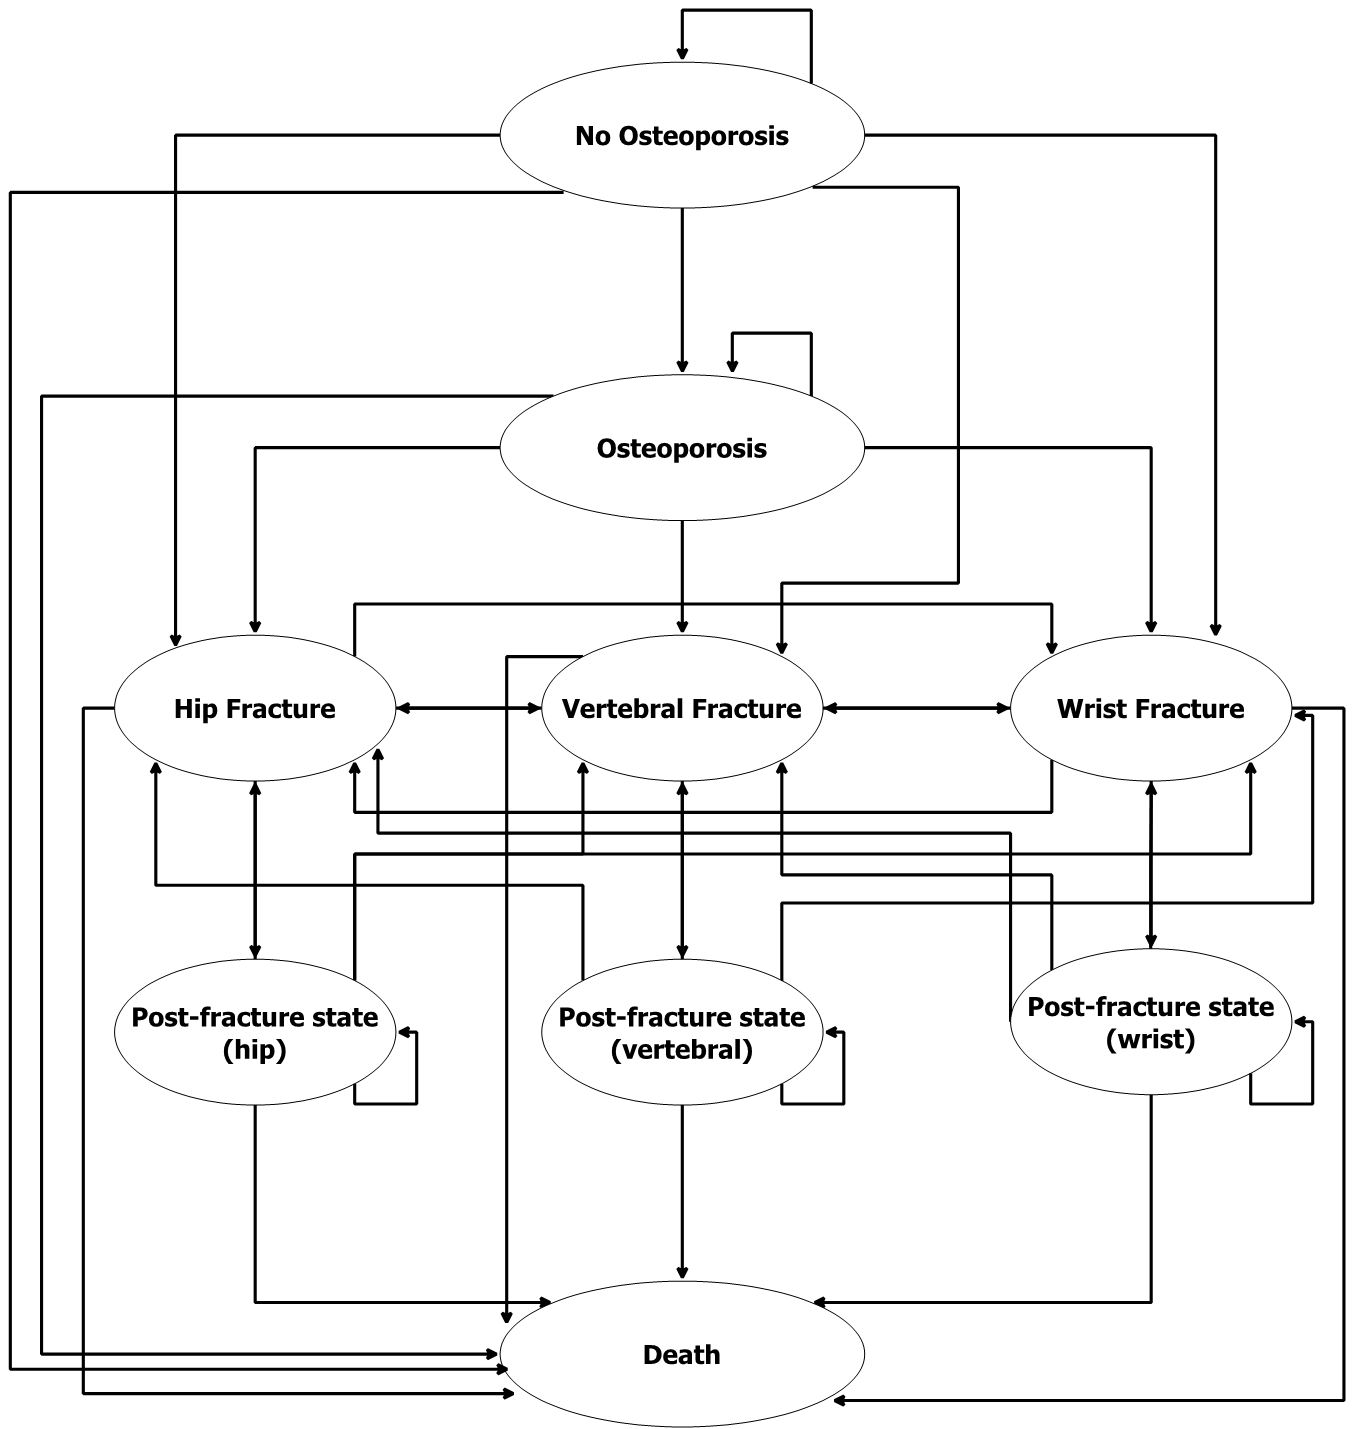
\includegraphics[width=0.8\textwidth]{4-2.png}
\caption{Structure of the Microsimulation Model.}
\label{fig:4-2}
\end{figure}

\subsection{Validation of the Individual-level Model}

The internal and external validation for the model were conducted based on guidelines from ISPOR \cite{4-24}. For internal validation, validation output generated from the model was used to compare with real, observed values from among the data used for creating the model. The prevalence of osteoporosis at different age groups were compared to assess the degree to which the model reproduced the observed data. For external validation, simulated validation output were compared with observed data from sources that were not used in the creation of the model: life expectancy and lifetime probability of fracture in women older than 50 and 80 years. The performed Goodness-of-fit analysis was performed by fitting a linear relationship between modelled and observed data. Model validity was assessed via the squared linear correlation coefficient (R$^2$). These analyses were performed using SPSS@ Statistics Version 25. Detailed validation approaches are elaborated upon in the Appendix (Sections Interval Validation and External Validation).

\subsection{Two-dimensional Simulation}

We employed a two-dimensional simulation \cite{4-25}. The two dimensions were defined in terms of parameter-level iterations and individual-level iterations. The parameter-level iterations captured input parameter uncertainty for parameters that were relevant for groups of persons while the individual-level iterations (microsimulations) captured patient-level stochasticity. For each scenario consisting of a combination of starting age, screening interval and CT2S cost, 10,000 parameter-level iterations were ran. For each parameter-level iteration, model input parameters were sampled from distributions. With each set of input parameters, 1000 iterations of the individual-level model (microsimulations) were simulated as described above. Each sampled individual then entered the microsimulation model four times, once for each of the strategies. Lifetime costs and QALYs for each strategy were then averaged across individual-level iterations, and grand averages were computed as averages of the individual-level averages across parameter-level iterations. Distributions of the model outputs - average lifetime costs and QALYs among parameter-level iterations provided an estimate of the combined uncertainty related to input parameter uncertainty and patient stochasticity. Despite the lack of reported confidence intervals or standard deviations for the health utility, osteoporosis prevalence, mortality rate, and annual fracture rate for the Dutch general population, we incorporated these values into our parameter-level sampling by estimating beta distributions. The standard deviation was estimated to be 20\% of the mean (Table \ref{tab:4-1}).  Moreover, the screening interval and discount rates were considered to be fixed values.

\subsection{Cost-Utility Analysis}

Using the simulated data, we performed CUAs. For each starting age, screening interval, treatment and discount rates scenario, the grand averages for the four strategies (CT2S, DXA, Treat all and No Screening) were recorded. Incremental cost-effectiveness ratios (ICERs) were calculated as the difference in lifetime costs divided by the difference in QALYs between pairs of strategies. A strategy was considered cost-effective if the Incremental Cost-Effectiveness Ratio (ICER) was below the lower bound ICER threshold set in the Netherlands (\texteuro 20,000/QALY gained) \cite{4-26}. If a strategy had lower estimated lifetime cost yet higher QALYs than its comparator, it was considered to dominate the comparator.

To assess the uncertainty in the CUAs, the net monetary benefit (NMB) was calculated for each parameter-level iteration and each strategy as $\lambda^* \mathrm{QAL} \mathrm{Y}_{\mathrm{ij}}-\mathrm{C}_{\mathrm{ij}}$ where `$\lambda$' is the willingness-to-pay (WTP) threshold expressed as the average cost of generating one additional quality-adjusted life year in the Netherlands, `i' is the index of the parameter-level iteration, `j' is the index of the strategy (0 for No Screening, 1 for DXA, 2 for CT2S and 3 for Treat all). QAL $\mathrm{Y}_{\mathrm{ij}}$ and $\mathrm{C}_{\mathrm{ij}}$ represent the QALYs and average lifetime cost estimated for the ith iteration of the jth strategy, respectively. In order to illustrate combined parameter-level and person-level uncertainty, we constructed cost-effectiveness acceptability curves (CEACs) where the value of $\lambda$ was varied, and at each value, the proportions of parameter-level iterations for which each strategy had the highest NMB was determined. The cost-effectiveness acceptability frontier (CEAF) was also constructed for comparison.

\subsection{One-Way Sensitivity Analysis}

We performed deterministic one-way sensitivity analysis (DSAs) to study the impact changes of each input parameter on the simulation results when all other input parameters were sampled as per usual. Screening sensitivity and specificity, fracture cost, fracture risks, discount rates, treatment efficacy, medication cost, excess mortality, fracture disutilities, screening interval and screening cost were included in the one-way sensitivity analyses. In each DSA, most of the given parameter varied from 80 to 120\% of its base case value \cite{4-27}. In order to reflect more uncertainty of the CT2S test characteristics, we expanded the sensitivity analyses of the CT2S test characteristics (both sensitivity and specificity) by varying the value from 70\% to 130\%, and incorporating more finely-grained intervals (10\%). The discount rate of effectiveness and cost were varied from 0\% to 6\%. The screening interval varied from 3 to 7 years. The gradient in average lifetime cost and the QALYs across the range of values employed for the DSA for No Screening, DXA, CT2S and Treat all were estimated for each input parameter.

\subsection{Model Input Parameter Data}
\subsubsection{Medication and Efficacy}

The bisphosphonate alendronate is the most frequently prescribed medication for osteoporosis in the Netherlands \cite{4-28}, weekly oral alendronate has been adopted in our base case analysis, together with the combination of vitamin D, calcium and lifestyle recommendation \cite{4-29}. Once-yearly intravenous infusion of zoledronic acid has become a popular alternative to oral alendronate for treating osteoporosis in postmenopausal women. This treatment has better adherence and similar effectiveness in reducing the risks of different types of fractures \cite{4-30,4-31} . Therefore as part of our scenario analyses, annual zoledronic acid treatment was also considered. The relative risk (RR) of osteoporotic fracture with alendronate and zoledronic acid treatment are presented in Table \ref{tab:4-1} \cite{4-31,4-32,4-33}.

\subsubsection{Treatment Duration and Adherence}

Based on the NHS guidance in the UK, it may take 6 to 12 months for alendronate to be fully effective in terms of bone protection \cite{4-34}. Since the cycle length of our simulation was 1 year, we assumed no treatment efficacy if the treatment was discontinued within the first year. Several studies have recommended applying a `drug holiday' after 5 years of continuous alendronate treatment, which is in accordance with evidence to show that the residual effect of the alendronate will be sustained for up to 5 years \cite{4-35,4-36}. Therefore, we assumed that the maximum duration of continuous alendronate prescription was 5 years with a residual effect that declined linearly to 0 over a 5-year period after treatment was discontinued \cite{4-37}. Two studies of alendronate treatment in postmenopausal women with osteoporosis showed that 69\% of people remained on treatment after 1 year \cite{4-38} while 18.2\% received the full 5 years of treatment \cite{4-39}. We assumed the percentage of people staying on treatment declined in a linear manner and calculated the discontinuation rate of alendronate treatment from year 1 to 5.

A study of the effect of zoledronic acid treatment shows that there is no significant difference in treatment efficacy between the patients with 6 versus 9 years of treatment \cite{4-40}. Since the residual effect of zoledronic acid could be up to 3 years \cite{4-30}, we assumed that the maximum duration of continuous alendronate treatment was 6 years and the residual effect of zoledronic acid will be declined in linear manner to 0 over a 3-year period after treatment was discontinued. Only one study of zoledronic acid reported the yearly percentage of patient stay on treatment from year 1 to 4 \cite{4-41}. We made the assumption that the proportion of patients who remained on the treatment would decrease in a linear fashion for year 5 and 6. For both alendronate and zoledronic acid treatment, re-treatment was modelled to be provided if a fracture occurred or the rescreening result was positive. Treatment was also provided to woman who initially screened negative but subsequently screened positive.

\subsubsection{Osteoporosis Prevalence and Incidence}

Osteoporosis-related studies revealed that the prevalence of osteoporosis in the Netherlands is 1.9 per 1000 for men and 16.1 per 1000 for women and increases with age \cite{4-29,4-42}. However, specific osteoporosis prevalence data for elderly women across age groups were not available for the Dutch population. Therefore, data from a Swedish population study was employed \cite{4-43}. Since the current study is focused on Dutch postmenopausal women referred to the FLS, the Swedish data were supplemented with the reported osteoporosis prevalence of the people referred to the FLS in the Netherlands \cite{4-44}. Due to the fact that the osteoporosis prevalence of the 5 FLSs study were not reported by sex, the model's osteoporosis prevalence estimate (40.7\%) was obtained for women within the 70s age group from the FLS with the highest proportion of female persons (88.2\%), which also had an average age of 69 \cite{4-44}. Since data from the Netherlands FLS lacked detailed osteoporosis prevalence for the 60s and 80s age group for women, the increment in the osteoporosis prevalence of the general population was used and the osteoporosis prevalence were estimated to be 25.7\% and 55.2\% for each of the age groups, respectively (Table \ref{tab:4-1}). The incidence of osteoporosis based on the difference of osteoporosis prevalence plus the mortality rate for the specific age group was estimated \cite{4-45}. We considered the differences in the prevalence of osteoporosis as 5-year cumulative osteoporosis incidence to calculate the 1-year incidence rate and transition probability of developing osteoporosis \cite{4-46}. Detailed calculations of osteoporosis transition probability are elaborated upon in the Appendix (Section Transition Probability of Developing Osteoporosis).

\subsubsection{Fracture Rates}

The age-specific annual hip, vertebral and wrist fracture rates were obtained for general population from the Dutch-specific osteoporosis reports by the International Osteoporosis Foundation (IOF) \cite{4-47}. We calculated the annual osteoporotic fracture incidence rate using the annual incident rate of fracture for the general population times Melton's osteoporosis attributed rates \cite{4-48} and then divided by the prevalence of osteoporosis for that age band. Subsequently, the annual incidence rate was translated to transition probability using equation 2 shown in Appendix \cite{4-46}. Since all people in FLS had a previous history of fracture, the fracture rates for people experiencing `first fracture' in our simulation were adjusted by multiplying the relative risks (RRs) of any secondary fracture for people with a previous fracture history (1.86 according to Kanis's study) \cite{4-49}. Simulated people in our model could suffer more than one fracture and the risk of sustaining a subsequent fracture was therefore set higher than the initial fracture risk. The RRs of secondary hip, vertebral and wrist fractures were therefore obtained as 2.9, 2.52 and 1.69, respectively \cite{4-50,4-51}. The corresponding transition probabilities of fractures per cycle are calculated based on the annual fracture rates \cite{4-46}. Detailed age specific annual fracture rates and the calculations of the osteoporotic fracture probabilities are elaborated in the Appendix (Section Fracture rates for Dutch general population and osteoporotic fracture rates calculations).

\subsubsection{Mortality Rate}

Consistent with the previous economic evaluations of  secondary fracture prevention intervention \cite{4-52}, age-specific, general population mortality risks for Dutch women were derived from the Global Health Observatory data repository published by the World Health Organisation (WHO) as our baseline mortality rates \cite{4-53}. Mortality risk of osteoporotic individuals were higher than the general population (RR= 1.19), this value has been applied to the patients having osteoporosis but without experiencing `first fracture' in our simulation \cite{4-54}. The relative mortality risk of people with and without hip fractures within the general population is 2.87 and 1.78 for the first and subsequent years, respectively \cite{4-55}. Several studies have shown that the excess mortality rate after vertebral fracture is similar to those of hip fracture \cite{4-56,4-57,4-58}. Therefore in the model, the relative mortality risk after vertebral and hip fracture was assumed to be the same. Excess mortality rate after wrist fracture was estimated to be 1.43 \cite{4-59}. Since comorbidities could also be a contributing factor to excess mortality, the proportion of the excess mortality following fractures attributable to the fractures themselves was assumed to be 25\% \cite{4-60,4-61}, therefore, the excess mortality of hip, vertebral, and wrist fractures have been adjusted accordingly to avoid overcounting. Besides, consistent with the previous economic evaluations of osteoporosis intervention \cite{4-62}, the model considers only the additional mortality caused by hip or vertebral fractures in patients who have experienced both non-hip/non-vertebral fractures and hip/vertebral fractures. In the case of patients who have multiple hip or vertebral fractures, or both types of fractures, only one excess mortality value was included in the model.

\subsubsection{Costs}

The following cost items were considered in our model: direct cost of fractures, annual medication cost, screening cost and nursing home costs after hip fracture. In the first year post fracture, the direct costs associated with hip, vertebral and wrist fracture in the Netherlands were reported to be \texteuro 21,477, \texteuro 2,740 and \texteuro 1,573, respectively \cite{4-63,4-64,4-65}. A study revealed a substantial rise in the use of generic alendronate among the Dutch population since its availability in 2005, with up to 62\% of patients opting for this medication by 2011 \cite{4-66}. Furthermore, the Dutch health insurance companies tend to reimburse more affordable generic form of drug. Therefore, our study incorporated the annual cost of generic alendronate in the Netherlands \cite{4-67}. When a hip fracture occurred, patients either entered into a nursing home or the community for recovery and the corresponding transition probabilities have been applied \cite{4-68,4-69}. The annual cost of nursing home residence (\texteuro 63,549) was calculated using the subtraction of the total cost of a person with a hip fracture confined to a nursing home and the first-year direct cost of hip fracture \cite{4-70}. The DXA scan price in the Netherlands is \texteuro 96.74 \cite{4-64}. The cost of the CT2S screening was calculated with the following components: CT scan cost, computing cost, storage cost of raw data, licence cost and personnel cost. The average cost of CT2S screening was estimated to be \texteuro 274 (Table \ref{tab:4-3}, Appendix). All costs were adjusted for the inflation rate in the Netherlands to the 2022 value \cite{4-71}. We assumed everybody received sufficient calcium and vitamin D so the costs of supplements were not included in the model.


\begin{center}
\centering
%\setlength{\tabcolsep}{0.8mm}{
\begin{longtable}{lllll}
\caption{Lifetime healthcare costs, QALYs, averaged across simulation iterations and incremental cost-effectiveness ratio of CT2S compared with DXA, Treat all and No screening for the various age groups under the base case scenario: weekly oral alendronate treatment, screening interval = 5 years, discount rates are 4.0\% and 1.5\% for costs and effectiveness.}
\label{tab:4-2}\\
\toprule
 & {\bf CT2S} & {\bf DXA} & {\bf Treat all} & {\bf No screening}\\
\midrule
{\bf Women aged 60-70 y} &   &   &   &  \\
Cost & \texteuro  7,177 & \texteuro  6,765 & \texteuro  7,082 & \texteuro  7,694\\
QALY & 14.080 & 14.070 & 14.025 & 13.998\\
ICER &   & \texteuro  41,200 & \texteuro  1,727* & Cost-saving\\
{\bf Women aged 70 $-$80 y}  &   &   &  \\
Cost & \texteuro  9,768 & \texteuro  9,599 & \texteuro  10,216 & \texteuro  11,338\\
QALY & 9.491 & 9.479 & 9.449 & 9.403\\
ICER &   & \texteuro  14,083* & Dominant & Cost-saving\\
{\bf Women aged 80 $-$90 y}  &   &   &  \\
Cost & \texteuro  13,553 & \texteuro  13,712 & \texteuro  13,534 & \texteuro  16,520\\
QALY & 5.286 & 5.275 & 5.274 & 5.212\\
ICER &   & Dominant & \texteuro  1,583* & Cost-saving\\
\bottomrule
\end{longtable}%}
\begin{tablenotes}
\footnotesize
\item[a] Dominant = CT2S more QALYs, lower costs than DXA or Treat all. Cost-saving = CT2S more QALY and lower costs than No screening 
\item[b] *Using the lower bound of WTP threshold in the Netherlands (\texteuro 20,000), these values are considered cost-effective for CT2S compared against DXA or Treat All
\end{tablenotes}
%\vspace{-2.5em}
\end{center}


\begin{center}
\centering
\setlength{\tabcolsep}{0.8mm}{
\begin{longtable}{m{6cm}m{2cm}<{\centering}m{2.3cm}<{\centering}m{1.8cm}<{\centering}}
\caption{One-way sensitivity analyses on the incremental cost-effectiveness ratio of CT2S vs No screening, CT2S vs DXA, and CT2S vs Treat all for the 70s age group under the base case scenario: with weekly oral alendronate treatment and 5 years screening interval, discount rates 4.0\% and 1.5\% for costs and effectiveness.}
\label{tab:4-3}\\
\toprule
{\bf Parameters} & \multicolumn{3}{c}{{\bf ICER}} \\
\midrule
 & {\bf CT2S vs No screening} & {\bf CT2S vs DXA} & {\bf CT2S vs Treat all}\\
\midrule
{\bf Base case} & Cost-saving & 14,083 & Dominant\\
\midrule
0.8 times DXA screening cost & Cost-saving & 20,214 & Dominant\\
1.2 times DXA screening cost & Cost-saving & 15,524 & Dominant\\
0.8 times Annual nursing home cost & Cost-saving & 18,571 & Dominant\\
1.2 times Annual nursing home cost & Cost-saving & 12,476 & Dominant\\
0.8 times DXA screening sensitivity & Cost-saving & Dominant & Dominant\\
1.2 times DXA screening sensitivity & Cost-saving & 112,711 & Dominant\\
0.8 times DXA screening specificity & Cost-saving & 17,850 & Dominant\\
1.2 times DXA screening specificity & Cost-saving & 13,265 & Dominant\\
0.7 times CT2S screening sensitivity & Cost-saving & Dominated by DXA & 3,984\\
0.8 times CT2S screening sensitivity & Cost-saving & Dominated by DXA & Dominant\\
0.9 times CT2S screening sensitivity & Cost-saving & 24,751 & Dominant\\
1.1 times CT2S screening sensitivity & Cost-saving & 2,870 & Dominant\\
1.2 times CT2S screening sensitivity & Cost-saving & Dominant & Dominant\\
1.3 times CT2S screening sensitivity (sensitivity = 1\dag) & Cost-saving & Dominant & Dominant\\
0.7 times CT2S screening specificity & Cost-saving & 5,234 & Dominant\\
0.8 times CT2S screening specificity & Cost-saving & 8,937 & Dominant\\
0.9 times CT2S screening specificity & Cost-saving & 12,956 & Dominant\\
1.1 times CT2S screening specificity & Cost-saving & 15,173 & Dominant\\
1.2 times CT2S screening specificity & Cost-saving & 20,834 & Dominant\\
1.3 times CT2S screening specificity (specificity = 1\dag\dag) & Cost-saving & 32,123 & Dominant\\
screening interval = 3 & Cost-saving & 34,957 & Dominant\\
screening interval = 7 & Cost-saving & 4,680 & Dominant\\
0.8 times CT2S screening cost & Cost-saving & 2,222 & Dominant\\
1.2 times CT2S screening cost & Cost-saving & 28,825 & Dominant\\
discount rate = 0\% & Cost-saving & 4,586 & Dominant\\
discount rate = 6\% & Cost-saving & 30,077 & Dominant\\
0.8 times Excess mortality attributable to fracture & Cost-saving & 16,210 & Dominant\\
1.2 times Excess mortality attributable to fracture & Cost-saving & 13,071 & Dominant\\
0.8 times alendronate persistence & Cost-saving & 24,029 & Dominant\\
1.2 times alendronate persistence & Cost-saving & 10,712 & Dominant\\
0.8 times annual fracture rate general population & Cost-saving & 20,557 & Dominant\\
1.2 times annual fracture rate general population & Cot-saving & 7,214 & Dominant\\
0.8 times Fracture disutilities & Cost-saving & 24,968 & Dominant\\
1.2 times Fracture disutilities & Cost-saving & 10,578 & Dominant\\
0.8 times Fracture cost & Cost-saving & 17,931 & Dominant\\
1.2 times Fracture cost & Cost-saving & 13,117 & Dominant\\
0.8 times base case treatment efficacy & Cost-saving & 27,109 & Dominant\\
1.2 times base case treatment efficacy & Cost-saving & 7,436 & Dominant\\
0.8 times annual medication cost & Cost-saving & 14,224 & Dominant\\
1.2 times annual medication cost & Cost-saving & 13,927 & Dominant\\
\bottomrule
\end{longtable}}
\begin{tablenotes}
\footnotesize
\item[a] Dominant = CT2S more QALYs, lower costs than DXA or Treat all. Dominated by DXA =  CT2S lower QALYs, more costs than DXA.  Cost-saving = CT2S more QALY and lower costs than no screening
\item[b] \dag Note tht the absolute value of sensitivity has exceeded 1 when CT2S screening sensitivity was increased by 30\%
\item[c] \dag\dag Note tht the absolute value of specificity has exceeded 1 when CT2S screening specificity was increased by 30\%
\end{tablenotes}
%\vspace{-2.5em}
\end{center}

\subsubsection{Health-State Utility Values}

The health utilities values were obtained from a previous application of the EQ-5D multidimensional health index to a sample from the general population in the Netherlands, responses on the five domains of the index were mapped to utility values using the European VAS value set scoring algorithm \cite{4-72}. The baseline health-state utility values for patients with prior fractures were estimated by multiplying the health-state utility of the general population by 0.85, a health utility multiplier for subsequent years ($> 2$ years) after a prior vertebral fracture. This is consistent with the previous economic evaluations of fracture liaison services patients \cite{4-52}. Since fractures and post fracture recovery will be associated with a decline in quality-of-life, we applied a health utility multiplier of the subsequent years after fractures in our simulation \cite{4-73}. In addition, the health utility of 0.4 was used for those people entering nursing homes after a hip fracture \cite{4-74}.

\section{Results}
\subsection{Internal and External Validation Results}

For internal validation, the modelled and observed prevalence of osteoporosis were compared. The squared correlation coefficient (R2) was 0.998. For external validation, the R$^2$ was jointly calculated for life expectancy and fracture risk and the value was 0.988. The collective results are shown in Table \ref{tab:4-1} and Table \ref{tab:4-2} in the supplemental Appendix.

\subsection{Base Case Analysis}

Grand averages of lifetime costs and QALYs, as well as cost-utility analyses results are presented in Table \ref{tab:4-2}. In the base case analysis, the screening interval was set to 5 years, with discount rates of 4.0\% for costs and 1.5\% for effectiveness (according to the Dutch guideline for economic evaluations in healthcare). The treatment strategy involved weekly oral alendronate treatment. The ICERs of CT2S vs. DXA for the age groups of 60s and 70s were \texteuro 41,200 and \texteuro 14,083, respectively, per QALY gained. For the 80s age group, CT2S was dominant (an increase in QALYs at lower lifetime cost) compared with DXA screening. The ICERs of CT2S vs. Treat all strategy for the age groups of 60s and 80s were \texteuro 1,727 and \texteuro 1,583, respectively. For the 70s age group, CT2S was dominant compared with Treat all. In all simulated populations, CT2S was cost-saving (more effective and less costly)  compared to the No Screening scenario. According to the cost-effectiveness in practice published by the Dutch National Health Care Institute, the WTP threshold in the Netherlands varies from \texteuro 20,000 to \texteuro 80,000 \cite{4-26}. In this study, we conservatively used \texteuro 20,000 to evaluate the cost-effectiveness of the screening strategies across all populations and scenarios. The results indicated that ICER of CT2S vs. DXA for the 70s and 80s age groups is less than the lower bound ICER threshold (\texteuro 20,000) in the Netherlands. It is worth mentioning that the QALY outcomes of the Treat all strategy without screening are always lower than those with screening. Treatment adherence is considered in our model and the lifetime horizon simulation also simulates the progression of patients developing osteoporosis. Even though Treat all strategy treat all patients referred to the FLSs at the beginning, the rescreening process can identify those patients who developed osteoporosis after treatment discontinuation. The targeted treatment will impact the final outcomes of QALY and cost for each individual patient referred to the FLSs. However, we observed that the gap in QALY outcomes between the Treat all strategy and CT2S or DXA screening diminishes as the simulation group ages. This is largely due to the increase in osteoporosis prevalence in the older age group and shorter simulated lifetime.

\subsection{One-Way Sensitivity Analysis}

Table \ref{tab:4-3} reported the result of one-way sensitivity analysis in women in their 70s using the base case scenario: with the screening interval of 5 years, discount rates at 4.0\% and 1.5\% for costs and effectiveness with weekly oral alendronate treatment. In all the sensitivity analyses, CT2S was cost-saving compared with No Screening scenario. Furthermore, CT2S dominated Treat all strategy in most of the sensitivity analyses, except when CT2S sensitivity was at $-$30\%. In that case, the ICER of CT2S versus Treat all was \texteuro 3,984.  

When comparing CT2S with DXA, the CT2S sensitivity had a marked impact on the ICER outcome. When CT2S sensitivity increased by 10\%, the ICER of CT2S vs. DXA was \texteuro 2,870. When CT2S sensitivity increased by 20\% and 30\%, CT2S dominated DXA. On the contrary, when CT2S sensitivity decreased by 10\%, the ICER of CT2S vs. DXA was \texteuro 24,751. When CT2S sensitivity decreased by 20\% and 30\%, DXA dominated CT2S. This is expected as the sensitivity of CT2S decreases (by 20\% or more), its ability to identify osteoporosis patients reduces, making it less superior compared with DXA.  Similarly, When DXA sensitivity decreased by 20\%, the CT2S method became dominant compared with DXA. Conversely, when the sensitivity of DXA increased by 20\%, the ICER of CT2S vs. DXA increased to \texteuro 112,711.

The results were also strongly affected by other parameters such as screening interval and the cost of CT2S. The ICER of CT2S compared to DXA more than doubled when the screening interval was equal to 3 years. The ICER of CT2S vs. DXA decreased to \texteuro 2,222 when the CT2S cost decreased by 20\%. Moreover, the ICER of CT2S vs. DXA increased to \texteuro 27,109 if the medication efficacy decreased by 20\%. The decrease in medication persistence resulted in lower QALY and higher cost and changed the ICER of CT2S vs. DXA to \texteuro 24,029. Cost per QALY increased to \texteuro 30,077 when the discount rate increased to 6\% and decreased to \texteuro 4,586 when the discount rate decreased to 0\%, respectively. Additionally, when the specificity of CT2S varied from $-$30\% to $+$30\%, the ICER continued to increase. 

\subsection{Alternative Scenario Analyses}

As an extension to the base case scenario, we extended our analysis to also consider: (a) alternative discount rate (3\% rate for benefits as well as costs used in other countries), (b) alternative treatment of once-yearly intravenous infusion of zoledronic acid, and (c) alternative screening interval of 2 years in the scenario analyses. The results for these alternative scenarios were presented in Table \ref{tab:4-4}.

\begin{center}
\centering
%\setlength{\tabcolsep}{0.8mm}{
\begin{longtable}{lllll}
\caption{ICER of CT2S screening compared with DXA, Treat all and No Screening with three alternative scenarios: discount rate = 3\%, annual zoledronic acid treatment and 2-year screening interval scenarios. For each alternative scenario, the other parameters were kept the same as the base case scenario.}
\label{tab:4-4}\\
\toprule
 & {\bf CT2S} & {\bf DXA} & {\bf Treat all} & {\bf No screening}\\
\midrule
\multicolumn{4}{l}{{\bf (a) Discount rate = 3\%}}\\
\midrule
{\bf Women aged 60-70 y} &   &   &  &  \\
Cost & \texteuro  8,666 & \texteuro  8,235 & \texteuro  8,692 & \texteuro  9,459\\
QALY & 11.962 & 11.954 & 11.925 & 11.900\\
ICER &   & \texteuro  53,875 & Dominant & Cost-saving\\
{\bf Women aged 70 -80 y} &   &   &  &  \\
Cost & \texteuro  11,041 & \texteuro  10,888 & \texteuro  11,626 & \texteuro  12,894\\
QALY & 8.462 & 8.452 & 8.431 & 8.390\\
ICER &   & \texteuro  15,300* & Dominant & Cost-saving\\
{\bf Women aged 80 -90 y} &   &   &   &  \\
Cost & \texteuro  14,267 & \texteuro  14,448 & \texteuro  14,322 & \texteuro  17,431\\
QALY & 4.923 & 4.913 & 4.914 & 4.857\\
ICER &   & Dominant & Dominant & Cost-saving\\
\midrule
\multicolumn{4}{l}{{\bf (b) Annual zoledronic acid treatment}}\\
\midrule 
{\bf Women aged 60-70 y} &   &   &   &  \\
Cost & \texteuro  6,998 & \texteuro  6,626 & \texteuro  7,023 & \texteuro  7,674\\
QALY & 14.111 & 14.093 & 14.034 & 13.991\\
ICER &   & \texteuro  20,667 & Dominant & Cost-saving\\
{\bf Women aged 70 -80 y} &   &   &   &  \\
Cost & \texteuro  9,511 & \texteuro  9,397 & \texteuro  10,120 & \texteuro  11,340\\
QALY & 9.529 & 9.510 & 9.469 & 9.404\\
ICER &   & \texteuro  6,000* & Dominant & Cost-saving\\
{\bf Women aged 80 -90 y} &   &   &   &  \\
Cost & \texteuro  13,005 & \texteuro  13,269 & \texteuro  13,228 & \texteuro  16,484\\
QALY & 5.314 & 5.299 & 5.293 & 5.211\\
ICER &   & Dominant & Dominant & Cost-saving\\
\midrule
\multicolumn{4}{l}{{\bf (c) Screening interval = 2 years}}\\
\midrule
{\bf Women aged 60-70 y} &   &   &   &  \\
Cost & \texteuro  7,886 & \texteuro  6,682 & \texteuro  7,078 & \texteuro  7,694\\
QALY & 14.109 & 14.097 & 14.018 & 13.991\\
ICER &   & \texteuro  100,333 & \texteuro  8,879* & \texteuro  1,627*\\
{\bf Women aged 70 -80 y} &   &   &   &  \\
Cost & \texteuro  9,909 & \texteuro  9,131 & \texteuro  10,202 & \texteuro  11,325\\
QALY & 9.525 & 9.511 & 9.449 & 9.403\\
ICER &   & \texteuro  55,571 & Dominant & Cost-saving\\
{\bf Women aged 80 -90 y} &   &   &   &  \\
Cost & \texteuro  13,068 & \texteuro  12,879 & \texteuro  13,550 & \texteuro  16,527\\
QALY & 5.310 & 5.298 & 5.275 & 5.211\\
ICER &   & \texteuro  15,750* & Dominant & Cost-saving\\
\bottomrule
\end{longtable}%}
\begin{tablenotes}
\footnotesize
\item[a] Dominant = CT2S more QALYs, lower costs than DXA or Treat all. Cost-saving = CT2S more QALY and lower costs than no screening
\item[a] *Using the lower bound of WTP threshold in the Netherlands (\texteuro 20,00), these values are considered cost-effective for CT2S compared against DXA, Treat All or No screening  
\end{tablenotes}
%\vspace{-2.5em}
\end{center}

In the 3\% discount rate scenario (screening interval = 5 years, weekly oral alendronate treatment), the ICER of CT2S vs. DXA in the 60s age group was \texteuro 53,875, which exceeded the willingness-to-pay (WTP) threshold of the Netherlands (\texteuro 20,000). For the 70s age group,  the ICER of CT2S vs. DXA was \texteuro 15,300 per QALY gained. CT2S dominated DXA screening in the 80s age group. In all simulated populations, CT2S dominated Treat all scenario and was cost-saving compared to No screening. It is worth mentioning that Treat all strategy dominated DXA screening in the 80s age group (an increase in QALYs at lower lifetime cost as shown in the table). 

In the scenario with annual zoledronic acid treatment (screening interval = 5 years, discount rates are 4.0\% and 1.5\% for costs and effectiveness), the ICERs of CT2S versus DXA for the age groups of 60s and 70s were \texteuro 20,667 and 6,000, respectively, which were substantially lower than those in the base case analyses. However, the ICER for the 60s age groups was still higher than WTP threshold of the Netherlands. CT2S was dominant compared to DXA screening in the 80s age group. In all simulated populations, CT2S again dominated Treat all scenario and was cost-saving compared to No screening. 

In the scenario with a 2-year screening interval (weekly oral alendronate treatment, discount rates are 4.0\% and 1.5\% for costs and effectiveness), similar to the base case analysis, CT2S was cost-saving compared to the  No Screening scenario in age groups 70s and 80s. QALYs for both screening strategies were increased, and the ICER of CT2S compared to DXA also increased substantially compared to the 5-year interval. The ICER of CT2S compared with DXA was higher than the ICER threshold in the Netherlands for the age groups 60s and 70s (\texteuro 100,333 and 55,571, respectively). For the 80s age group, the ICER of CT2S vs. DXA was \texteuro 15,750, which is different to the base case scenario in a way that CT2S no longer dominated DXA. CT2S dominated the Treat all scenario in the 70s and 80s age groups. For age group 60s, the ICER of CT2S vs. Treat all was \texteuro 8,879. 

\subsection{Probabilistic Sensitivity Analyses}

Fig. \ref{fig:4-3} showed the CEACs and CEAFs for DXA, CT2S, No screening, Treat all with  2 age groups (70s and 80s) and two treatment strategies (weekly oral alendronate and annual zoledronic acid treatment).The analysis considered a screening interval of 5 years, with discount rates of 4.0\% and 1.5\% for costs and effectiveness (used in the base case). CEAFs are highlighted as bold dashed line in dark grey. For women in their 70s, at the threshold of \texteuro 20,000 per QALY gained, CT2S screening was the most cost-effective strategy in 45\% of the simulations with weekly oral alendronate treatment, compared to 41\% for DXA, 13\% for Treat all  and 1\% for No Screening. When patient received annual zoledronic acid treatment, at the same WTP threshold, CT2S was the most cost-effective strategy in 56\% of the simulations, followed by DXA (37\%), Treat all (7\%) and No Screening (close to 0\%). For women in their 80s with weekly oral alendronate treatment, at the threshold of \texteuro 20,000, CT2S was cost-effective in 43\% of the simulations compared to 36\% for Treat all, 21\% for DXA and 0\% for No Screening. CT2S was the most cost-effective screening strategy at any WTP threshold when patient received annual zoledronic acid treatment for the 80s age groups.

\begin{figure}[!h]
\centering
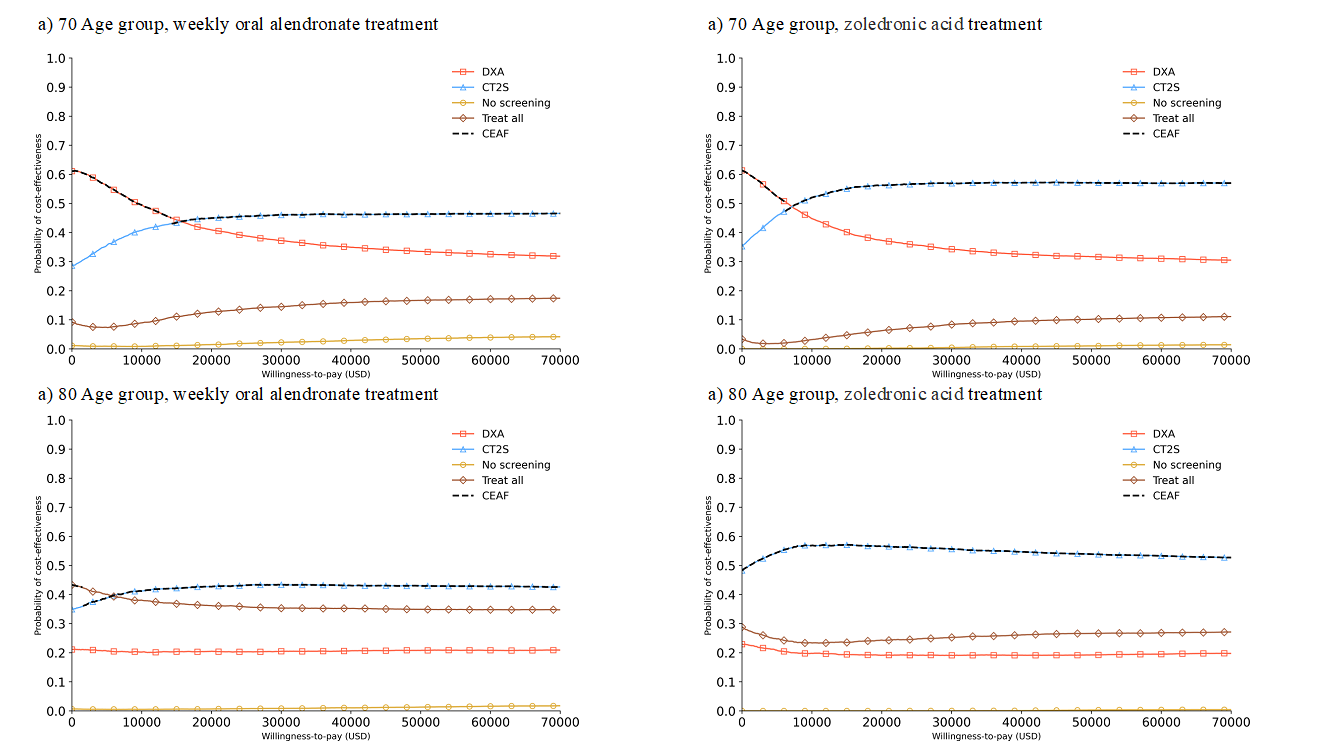
\includegraphics[width=1.0\textwidth]{4-3.png}
\caption{Cost-effectiveness acceptability curve and cost-effectiveness acceptability frontier for the 70s age group with weekly oral alendronate treatment (a) and zoledronic acid treatment (b). Cost-effectiveness acceptability curve for the 80s age group with weekly oral alendronate treatment (c) and zoledronic acid treatment (d). The other parameters are the same as the base case: screening interval = 5 years, discount rates are 4.0\% and 1.5\% for costs and effectiveness.}
\label{fig:4-3}
\end{figure}

\section{Discussion}

In this study, we applied early HTA to evaluate the cost-effectiveness of CT2S, DXA, Treat all, and No Screening strategies for osteoporosis screening and treatment in the Dutch postmenopausal women referred to FLS. These strategies were evaluated across various age groups, screening intervals, treatments, and discount rate scenarios. The aim of this research was to investigate the potential extra benefit, in terms of QALYs, and extra cost of a novel screening method, CT2S, in order to evaluate its potential economic attractiveness if adopted broadly among the FLS population in the Netherlands. To our knowledge, this was the first cost-effectiveness study for a fracture risk assessment tool using CT-based finite element model in osteoporosis screening. The findings suggest that compared to the current standard clinical approach DXA screening, CT2S has the potential to be cost-effective in women referred to Dutch FLS, especially for those within the 70s and 80s age groups. This finding of cost-effectiveness was also observed with a shorter osteoporosis screening interval of 2-years and an alternative treatment of annual zoledronic acid treatment with better adherence.

Our analysis has several strengths. The model structure allowed for realistic simulation of patients' osteoporosis case trajectories and inherently accounted for the competing risk of death. We conducted internal and external validation and showed that modelled validation output, prevalence of osteoporosis by age, lifetime risk of fracture and un-discounted, un-quality-adjusted life expectancy matched observed data quite well. In recent years, several cost-effectiveness studies have been conducted for osteoporosis screening (DXA and ultrasound) and treatment strategies \cite{4-45,4-75,4-76,4-77,4-78}. However, compared to Markov cohort models, we adopted a two-dimensional, we adopted a two-dimensional, discrete-state simulation methodology which offered two benefits. The large number of total iterations (parameter-level number multiplied by individual-level number) produced stable grand averaged lifetime costs and QALYs on which we performed our CUAs. The two-dimensional structure allowed us to assess the effect on the model output of the uncertainty surrounding input parameter point estimates as well as patient-level stochasticity expressed as cost-effectiveness acceptability curves.

To our knowledge, this was the first study in which DXA was not treated as the gold standard for osteoporosis screening (100\% accurate) since CT2S has been shown to have better discrimination between women with and without fractures. The current study addresses some of the limitations of the previous work. For example, the rescreening process was not considered in Mueller and Kingkaew's model \cite{4-75,4-77} and Li's model only considered rescreening with a 5-year screening interval \cite{4-45}. Our study considered both 5- and 2-year rescreening scenarios. In addition, Li's model only applied rescreening to people with previously negative results. However, the study by Van Gompel et al. \cite{4-19} showed approximately 60\% high-risk or osteoporotic women were re-screened within 5 years. Therefore, it was useful to simulate rescreening for all persons within FLS in the current study.

The classification accuracy of DXA and CT2S in identifying osteoporotic hip fractures has been used as the approximation of the osteoporosis screening accuracy in this study. Since osteoporotic fracture is one of the serious disease consequences of osteoporosis, and osteoporosis cannot be reversed without medication, it was reasonable to assume that the predictive accuracy cannot exceed the stratification accuracy of osteoporotic fractures for the same osteoporosis screening tool. If we treat the ``identification of osteoporosis'' was considered as finding those with a high risk of getting an osteoporotic fracture in the future, then we could treat the accuracy of the ``identification of osteoporosis'' could be treated as the predictive accuracy of getting an osteoporotic fracture in the coming 10 or 20 years. Therefore, if we use the stratification accuracy of osteoporotic fractures was used as an approximation to the identification of osteoporosis and prove it to be cost-effective, and hence elucidate that CT2S has the potential advantages in the identification of osteoporosis compared to DXA. 

The performance of CT2S, particularly its ability to accurately identify patients with osteoporosis (sensitivity), has a substantial impact on the ICER outcome, as indicated by the results of our one-way sensitivity analyses. Previous studies in the group have validated the CT2S approach using cadaver bones, which resulted in a 7-15\% standard error for failure strength and strain estimation when compared against experimental results \cite{4-6}. Part of this was attributed to the inter- and intra-observer error during the femur segmentation process, which was quantified to be within 5\%. The ARF0 (CT2S with added subject-specific fall dynamics and hip impact mechanics) was also verified with respect to all numerical approximations and achieved an overall error tolerance of 1.92 percentage points with an uncertainty of 4 percentage points due to model inputs \cite{4-6}. The CT2S input data used in this study has been carefully considered by taking results derived from the most appropriate boundary conditions to minimise potential error propagation \cite{4-7}. The range of values considered in the one-way sensitivity analysis here therefore represents the absolute worst case scenario when CT2S screening sensitivity was reduced by 20\% and 30\%, which are higher than the error range reported in previous sensitivity analyses. Future uncertainty quantification of CT2S input parameters will provide a more comprehensive understanding of its performance and enhance the robustness of cost-effectiveness analyses. Such studies could also be extended to include the application towards predicting other types of osteoporotic fractures like vertebral and wrist fractures. As early HTA analyses do not yield definitive recommendations for the development or adoption of innovations, their purpose is to contribute to ongoing discussions regarding investments, financial accountability, and reimbursement policies \cite{4-12}. In this context, our observations can contribute to the discourse surrounding the development, implementation, and reimbursement of CT2S as a potential novel osteoporosis screening tools for secondary fracture prevention.

In the current study, fixed screening intervals were adopted for both DXA and CT2S screening (5 and 2 years). In the clinical practice, the screening interval depends on the presence of risk factors and age \cite{4-79,4-80}. However, our screening interval scenarios would be expected to encompass the likely range of screening intervals that might be employed in practice. In addition, we assumed all the people within FLS were willing to cooperate and perform rescreening in fixed screening interval. This assumption is reasonable given that women chose to attend FLS at the onset, but could limit the generalisation of the CUA results to osteoporosis screening in non-FLS clinics.

The current model considered three main fractures (hip, vertebral and wrist) in our model. Other types of fractures were not considered due to the lack of relevant clinical data. This might lead to the underestimation of the potential lifetime cost savings and increase in quality-adjusted life expectancy from the prevention of other types of osteoporotic fracture. However, considering other types of fractures would serve to lower ICER values, which would strengthen the current findings of cost-effectiveness. Since the CT2S service to-date has only been used in clinical research and has not been commercialised, there was no profit margin added to the cost of CT2S. However, our estimation of CT2S screening cost is conservative and it involved setting the mean of a gamma distribution from which a cost was selected for each parameter-level iteration. These distributions covered a range of possible CTS costs. Furthermore, the automation of the CT2S image pre-processing step using open-source convolutional neural network (such as U-Net) may further reduce the cost. 

This study has several other limitations. Since the nursing home admission probability after hip fracture for Dutch population is only available for age group 80s \cite{4-69}, the admission probabilities for age groups 60s and 70s were obtained from a Norway study \cite{4-68}. In addition, while the prevalence of osteoporosis among women is nearly ten times higher than that among men in the Netherlands \cite{4-29}, it would be highly valuable to also investigate the cost-effectiveness of CT2S screening for men. Moreover, since health utilities, osteoporosis prevalence, mortality rate, and annual fracture rates for the Dutch population are not reported with confidence intervals or standard deviations, distributions were created for these parameters by assuming a standard deviation of 20\% of the mean to account for the parameter uncertainty. These data can be updated when relevant information become available in the future. The current model assumes that treatment recommendations based on DXA screening rely solely on the T-score, whereas other factors such as smoking, glucocorticoid use, and alcohol intake can be combined with the T-score in other fracture risk predictors such as the FRAX score \cite{4-81}. Unfortunately, it was not possible to include the FRAX model in this study due to a lack of required clinical data.

According to statistical data from 2020 and the report by the International Osteoporosis Foundation, there were 618 hospitals in the Netherlands in 2020, with over 50\% of these hospitals having FLS programs \cite{4-82,4-83}. However, at the national level, there are only 256 CT scanners available \cite{4-84}. This limitation may impact the future adoption of CT2S in clinical settings. Furthermore, in terms of the radiation effects of CT scan on patients, according to the study of Viceconti et al. (2018), the CT2S service recommends a whole femur CT scan protocol that results in an effective radiation dose ranging from 1.3 to 3.2 mSv for females \cite{4-4}. However, it also highlights a recent study suggests that even more aggressive reductions can be implemented without compromising the predictive accuracy \cite{4-85}. The 2018 study also demonstrates that the risk reduction in death due to complications related to hip fractures through CT2S is nearly ten times greater than the additional risk of death resulting from the additional radiation exposure for elderly women \cite{4-4}. Therefore, the radiation effects were not incorporated into the health utility of the patient in our model. Finally, this study focuses on the cost-effectiveness of CT2S osteoporosis screening in Dutch postmenopausal women and may not be directly apply to other countries and healthcare systems without recalibration of some input parameters.

In conclusion, this study demonstrated how early HTA may be applied for a potential novel osteoporosis screening tool for secondary fracture prevention in the Netherlands. The findings suggest that CT2S has the potential to be cost-effective in women referred to Dutch FLS at ages 70 and 80, compared to DXA screening, as the ICER fell below the lower bound ICER threshold in the Netherlands. The finding of cost-effectiveness was also observed with a shorter osteoporosis screening interval of 2-years and alternative treatment (annual zoledronic acid treatment) with better adherence. These findings suggest that CT2S could be used as a potential osteoporosis screening tool in the clinical setting in the Netherlands. And maybe more importantly. It raises the prospect that how high performance computing enabled simulation applications might contribute to enhanced healthcare quality and potential cost savings.








%!TEX root = ../dissertation.tex

\begin{savequote}[75mm]
Another inspiring quote for this chapter
\qauthor{Another author maybe}
\end{savequote}


\chapter[HPC in Healthcare: Business Model Transformations]{High-performance computing in healthcare: Identifying business model evolution via large language model and topic modeling}

\lettrine[lines=3]{\textcolor{SchoolColor}{T}}{his paper investigates the impact of}
technological advancements on the evolution of business models, with a specific focus on the healthcare sector. Manual analysis of business models from numerous financial reports poses significant challenges due to its time-consuming nature. To address this, our study introduces an automated framework
for business report analysis, leveraging advanced large language model
(LLM) and topic modeling techniques to explore how business models in healthcare evolve with High performance computing (HPC) adoption. This framework enables
the extraction and in-depth analysis of the business model from various reports,
uncovering a trend towards technology-driven and patient-centric models. It also identifies a shift toward recurring revenue models, diminishing
dependence on traditional funding sources like government contracts. Furthermore, our findings emphasize the growing significance of data and technological intellectual property in shaping the business landscape of healthcare. These insights highlight the substantial changes brought about by HPC in the business and economic landscapes of healthcare, providing valuable guidance for strategic planning and investment decisions. This analysis advocates for the enhanced integration of HPC technologies in the healthcare sector to fully leverage its potential for innovation and improved patient outcomes.



\section{Introduction}\label{sec1}

High-performance computing (HPC) has emerged as a pivotal technology in transforming the healthcare domain from a business perspective, enabling advancements in patient care, operational efficiencies, and innovation~\cite{belle2015big, veerla2023hpc}. HPC's role in healthcare extends from accelerating drug discovery and genome research to enhancing computational methods for large-scale data analysis, directly impacting the quality, speed, and cost-effectiveness of healthcare services~\cite{CHEN20181241,jumper2021highly,schmidt2017next}. The synergy between HPC and biomedical informatics accelerates the development of Artificial Intelligence (AI) methods, facilitating the development of advanced diagnostic tools and
personalized medicine approaches, tailoring treatments to individual patient
profiles, which were previously unattainable~\cite{bastrakov2013high,molidor2003new,lightbody2019review}. HPC��s role in advancing medical research cannot be over stated. It enables researchers to conduct complex simulations and analyses, leading to breakthroughs in understanding diseases and developing new treatments~\cite{ge2013molecular,kharche2008simulation,perrin2010model}. Moreover, the intersection of cloud computing with HPC introduces a paradigm shift in managing healthcare data, offering scalable and flexible solutions that enhance the quality and accessibility of care~\cite{hussein2013healthcare,lo2016mobile}. This integration facilitates systematic performance management and quality of care across the healthcare system, leveraging cloud technology for superior interoperability and data management~\cite{muhammed2018ubehealth,eze2016leveraging}. Additionally, the application of HPC for medical monitoring, particularly during pandemics, illustrates its essential role in supporting healthcare systems by ensuring the efficient and timely processing of medical data, which is vital for patient care and management~\cite{dananjayan2020artificial,majeed2021applications}.

The integration of HPC within the healthcare sector highlights its potential to drive business innovation. Investigating the business models of companies adopting HPC in healthcare offers valuable insights into the sector's business and economic dimensions, and provides a comprehensive understanding of the current landscape and potential future directions~\cite{reim2020implementation,muhtarouglu2013business}. Such insights can inform strategic planning and investment decisions within healthcare businesses utilizing HPC, identifying promising areas for further exploration and development. In this research, we applied the Business Model Canvas (BMC) framework by Osterwalder and Pigneur to examine companies' business models through detailed perspectives derived from their annual reports and conducted separate analyses~\cite{osterwalder2010business}. However, the vast number of companies updating their business reports annually, combined with rapid technological progress, challenges the manual analysis of BMC, making it both difficult and time-consuming. As a result,  there's a clear need for an automated tool that can effectively analyze a large volume of text, converting them into meaningful insights for business or strategic decision-making in the healthcare sector. We adopt recently developed topic modeling algorithms Top2Vec~\cite{angelov2020top2vec}, to manage extensive text collections and automatically uncover topics with significant keywords for easy understanding. By examining the evolution of companies' business models in the healthcare sector before and after implementing HPC from various perspectives, we gain insight into how HPC is accelerating business model innovation in the industry.

In this study, we develop an automatic business report analysis framework to invistigate how HPC impacts the business model evolution of companies in the healthcare domain. The primary contributions of this work are twofold:

\begin{enumerate}
\item We developed an automatic business model analysis framework, from business report retrieval and analysis to visualizations to depict business model evolution from different perspectives based on BMC. This adaptable pipeline can be generalized to other domains by modifying the business report retrieval rules.
\item By implementing an automated business model analysis framework, this study explores the transformation trends in business models among companies integrating HPC into healthcare. Our analysis reveals notable shifts: the healthcare sector is embracing AI, analytics, and cloud computing, moving towards technology-driven models. Firms have become more patient-focused, targeting diverse markets and prioritizing direct engagement. There is a move towards recurring revenue models, which lessens dependence on government contracts. Significantly, data and technological intellectual property have become key resources, surpassing traditional manufacturing and patents. These observations offer meaningful direction for upcoming investments and the strategic development of HPC in the healthcare industry, aiding in decision-making and resource allocation.
\end{enumerate}

\section{Theoretical Background}\label{sec2}
\subsection{Business model analysis and business model canvas}\label{subsec2.1}

The study of business models began to evolve as a distinct field, offering an alternative to conventional management methodologies in the mid-1990s~\cite{massa2017critical,zott2011business}. Business model is a conceptual framework that outlines how a company creates, delivers, and captures value. Teece et al. describe a business model as the architecture of value creation, detailing how a company delivers value to customers and converts it into profits~\cite{teece2010business}. This framework encompasses the mechanisms of value creation, delivery, and capture, reflecting management's hypothesis about customer needs and organizational capabilities to meet these needs profitably. Baden-Fuller and Haefliger~\cite{baden2013business} expand on this by defining the business model as a system for identifying the customer base, engaging with their needs, delivering satisfaction, and monetizing the value created, which is fundamental for linking technological innovation with firm.

While the term ``business model" is used frequently in academic and professional discourse, its interpretation diverges among scholars~\cite{al2010developing,sorrentino2015term,massa2017critical}. Despite the varied definitions, the essence of business models consistently emphasizes the importance of value creation. Fundamental to these models are the resources and operational activities involved~\cite{morris2005entrepreneur}. The variance in conceptualizations has led to many ontologies and methods for business modeling in academic research. Given our research's emphasis on analyzing business models from a systemic perspective, BMC serves as a prime example of this approach~\cite{kamprath2012systematic,upward2013towards}.


BMC originally conceptualized by Osterwalder and Pigneur~\cite{osterwalder2010business}, has emerged as a strategic management and entrepreneurial tool that allows organizations to describe, design, challenge, and pivot their business model. It has proven to be a comprehensive approach to business models and the effectiveness of the BMC in analyzing business models is well-documented across various studies and applications~\cite{muhtarouglu2013business,mustaniroh2020analysis,muller2019business}. The canvas encapsulates the essence of a business's operational blueprint across nine components, seamlessly interconnected to highlight how companies create, deliver, and capture value. These components include Value Propositions, outlining the problem solutions or needs fulfillment offered; Customer Segments, which delineates the target audience; Channels, indicating how a business reaches its customer segments; Customer Relationships, defining the nature of the interaction with customers; Revenue Streams, identifying the income sources from value propositions successfully delivered; Key Resources, highlighting the assets essential for operations; Key Activities, describing the most important actions a business must undertake; Key Partnerships, pointing out the network of suppliers and partners that make the business model work; and Cost Structure, detailing the monetary consequences of operating under a particular business model~\cite{osterwalder2010business}. Together, these elements provide a comprehensive snapshot, not only facilitating a deep understanding of a business's functioning core but also serving as a dynamic blueprint for innovation and strategic adjustment. This framework has not only been pivotal in aiding startups and established enterprises in navigating the complexities of their operations but has also fostered a universal language for discussing business models in a structured and coherent manner

\subsection{Topic modeling techniques }\label{subsec2.1}

Topic modeling, a branch of unsupervised machine learning, is designed to identify latent thematic structures within text corpora~\cite{blei2012probabilistic}. It classifies documents into topics based on the frequency and co-occurrence of words, serving as a critical tool for managing large, unstructured datasets and facilitating exploratory data analysis~\cite{jacobi2018quantitative}. Key techniques include Latent Dirichlet Allocation (LDA)~\cite{blei2003latent}, Non-negative Matrix Factorization (NMF)~\cite{lee1999learning}, and Latent Semantic Analysis (LSA)~\cite{deerwester1990indexing}, which are employed across text mining, information retrieval, and the digital humanities~\cite{alghamdi2015survey,huang2018analyst,yi2009comparative,meeks2012digital}. The utility of topic modeling extends to various fields such as marketing, healthcare, and social sciences, to detect trends within vast literature, social media content and reports ~\cite{amado2018research,karas2022experiments,sarioglu2013topic}. LDA is arguably one of the most widely used algorithms for topic modeling. Despite its popularity, LDA faces challenges like data preprocessing and the difficulty of interpreting topics~\cite{maier2018applying,angelov2020top2vec}, leading to the exploration of alternatives like entity linking (EL)~\cite{10.1145/3126686.3126776}. Recent advancements have introduced deep learning techniques like Top2Vec~\cite{angelov2020top2vec}, which leverage doc2vec models to generate semantic vector representations of words, thereby enhancing topic identification and creating integrated vectors for topics, documents, and words. Comparative studies suggest Top2Vec often outperforms LDA in quality of results~\cite{egger2022topic,karas2022experiments}.

\section{Materials and methods}\label{sec2}

In this section, we offer a detailed overview of the data and analytical methodology utilized in our study. Figure~\ref{fig:5-1} presents the automated literature review framework, comprising four key phases: business report retrieval and extraction, BMC extraction, topic modeling, and visualization. Detailed descriptions of each phase are provided in the following subsections.

\begin{figure}[!h]
\centering
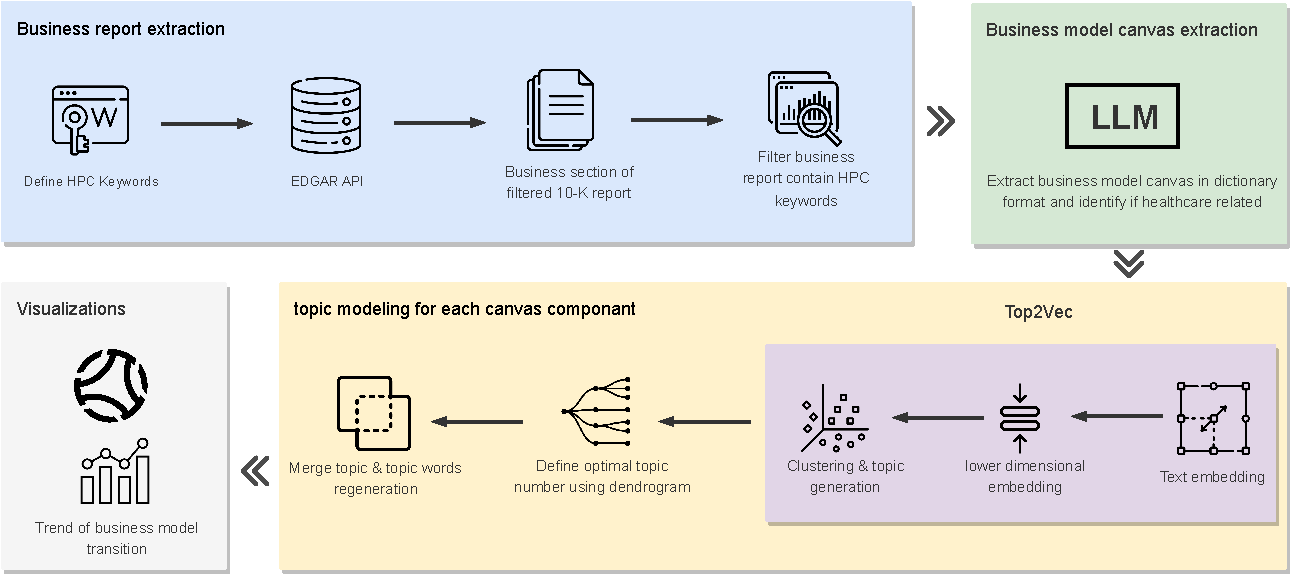
\includegraphics[width=0.95\textwidth]{5-1.pdf}
\caption{Automatic literature review pipeline consists of four stages: business report retrieval and extraction, BMC extraction, topic modeling, and visualization}
\label{fig:5-1}
\end{figure}

\subsection{Business report retrieval and extraction}\label{subsec2.1}
\subsubsection{Data source}\label{subsubsec2.1.1}

We propose to use the 10-K annual report in the analysis process. These reports are required by the U.S. Securities and Exchange Commission (SEC) for all publicly traded companies within the United States, serving as a comprehensive disclosure of their business operations and financial outcomes over the fiscal year\footnote{\url{https://www.sec.gov/files/form10-k.pdf}}. Public companies with significant assets are required to file these reports annually, contributing to a vast repository of over ten thousand documents available to the public. These documents are made publicly accessible through the Electronic Data Gathering, Analysis, and Retrieval (EDGAR) online database\footnote{\url{http://edgar.sec.gov}}, allowing for direct access via the EDGAR system's API\footnote{\url{https://www.sec.gov/edgar/sec-api-documentation}}. Given that the general filing deadline for 10-K reports is 90 days after the end of the fiscal year, and considering the timing of our research, filings for the year 2023 may not be fully complete. To guarantee the comprehensive collection of reports, we have limited our extraction to include filings up until the year 2022.

Each 10-K report is structured into 15 Items. The SEC's guidelines stress the significance of the description of business in Item 1 of the financial reports, which is of great interest for our research~\cite{securities2020modernization}. The guidance emphasizes the inclusion of pivotal aspects of a company's trajectory, such as historical development, strategic shifts, and current operational landscape. This information serves as a foundation for analyzing business models as it offers essential insights into various dimensions of the company's activities and intentions. Understanding the general development of the business, including detailed disclosures regarding revenue-generating activities, product development efforts, resource utilization, and regulatory compliance, illuminates the company's core operations and competitive positioning. In essence, the Item 1 section acts as a comprehensive narrative, providing vital context and insights crucial for understanding the company's strategic direction and competitive dynamics.

\subsubsection{HPC related business report retrieval pipeline}\label{subsubsec2.1.3}

We develop an automated pipeline for report retrieval and query expansion using the EDGAR API, initiating with the identification of HPC keywords, including `high performance computing', `supercomputing', and `cloud computing'. This initial set is iteratively expanded by incorporating additional relevant keywords derived from the reports, enabled through a keyword frequency analysis. Terms associated with HPC, appearing more than 50 times and not initially included, are added to the query. This method of automatic query expansion incorporates HPC-related synonyms and terms, such as `high-performance computing', `high performance computer', `supercomputer', `HPC cloud', `cloud services', and `cloud platform'. This process continues until no new significant keywords emerge, ensuring comprehensive coverage of the search area. Business reports identified through this refined search are then prepared for the subsequent analysis.

\subsection{Business model canvas extraction}\label{subsec2.2}

The business section of 10-K reports extracted in our study varies significantly in length, ranging from 1066 to 40406 words with an average word count of 6453, with key information pertaining to a company's BMC often concealed within the text. Applying topic modeling directly to extensive texts in thousands of documents does not effectively reveal transitions between different business model perspectives. Moreover, this approach lowers the analysis quality, as irrelevant text obscures essential keywords, complicating interpretation. Consequently, extracting information relevant to the nine components of the BMC becomes essential for a more targeted topic modeling process. However, manually reviewing hundreds of reports to construct a BMC for each is prohibitively time-consuming. Recent advances in large language models (LLMs) have demonstrated their effectiveness in zero-shot information extraction tasks, as highlighted by studies employing the GPT series models~\cite{kartchner2023zero,wei2023zero,hu2024zero}. Leveraging this advancement, we have designed prompts tailored for GPT-3.5 (\texttt{gpt-3.5-turbo-1106}) and GPT-4 (\texttt{gpt-4-1106-preview}) APIs\footnote{\url{https://platform.openai.com/docs/models/overview}},  chosen based on the length of the input text, to systematically extract the BMC from 10-K reports. the prompts are available at a public GitHub
repository\footnote{\url{https://github.com/tuohai1992/Business-model-canvas-topic-modeling/blob/main/Business_model_canvas_extraction_prompt.py}}. The outputs are organized in a format of python dictionary, detailing the nine essential components of the BMC. An example of this method is depicted in Figure~\ref{fig:5-2}, which presents the BMC extracted from the business section of Advanced Micro Devices (AMD)'s 10-K report, illustrating the GPT models' capacity to accurately identify and organize relevant information into the canvas structure.

\begin{figure}[!h]
\centering
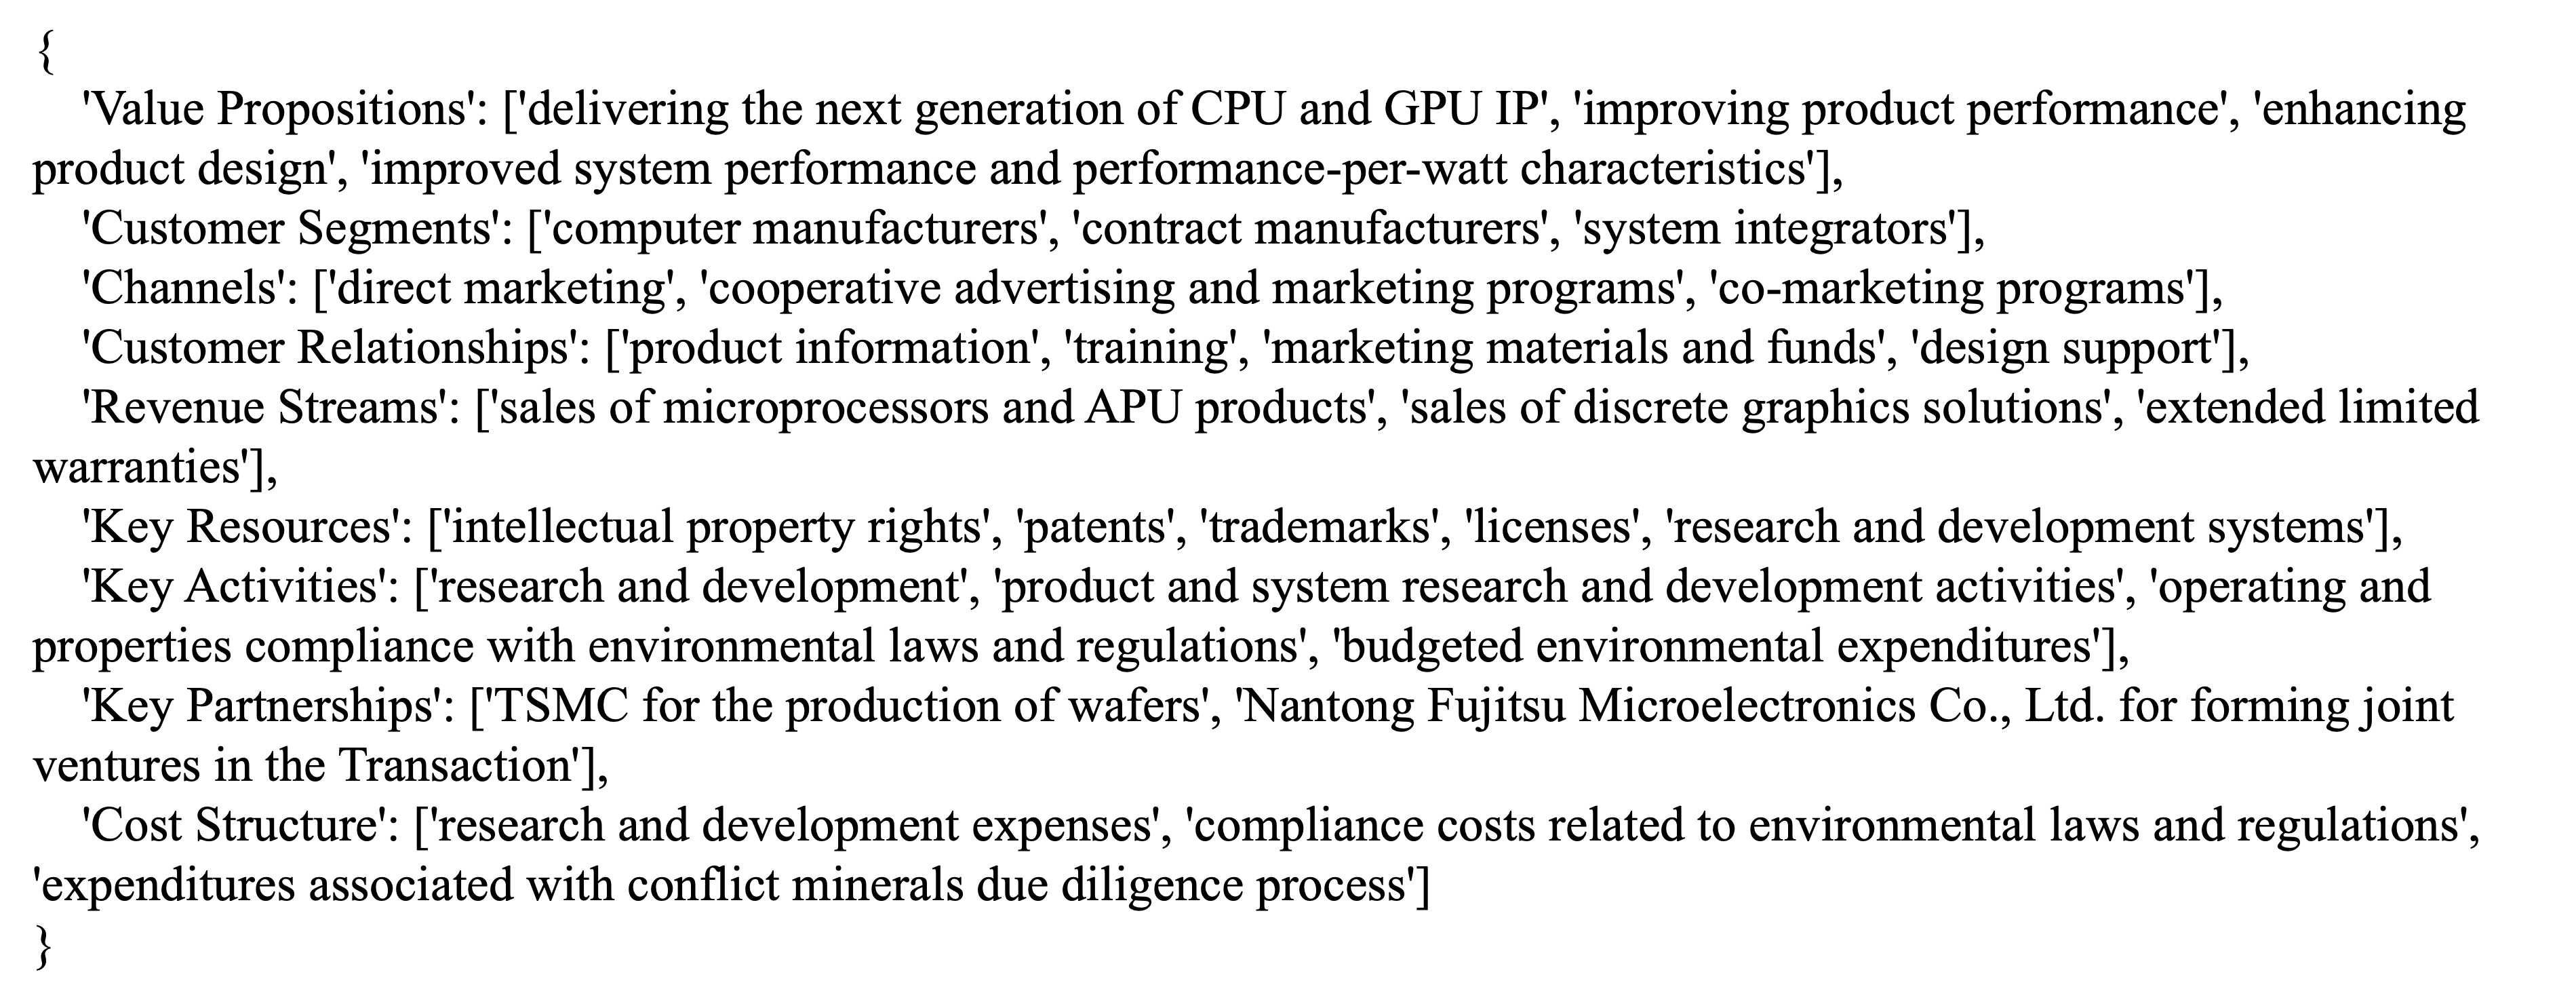
\includegraphics[width=0.95\textwidth]{5-2.png}
\caption{Example of business model canvas extracted by GPT-3.5 in a format of python dictionary}
\label{fig:5-2}
\end{figure}

\subsection{Identify healthcare related business model canvas}\label{subsec2.3}

Unlike extracting HPC-related business reports using specific HPC terminology, identifying keywords related to healthcare presents a broader and more generalized challenge. The determination of a company's involvement in the healthcare sector heavily relies on the semantic context. For example, references to `high performance computing' alongside `health' or `healthcare' in some business reports often pertain to system health, such as fault tolerance, job scheduling, and interconnection, rather than human health. The Standard Industrial Classification (SIC) Codes in a company's EDGAR filings are intended to identify its primary business line. However, despite many companies operating in multiple business lines, only one SIC code is assigned to each company in EDGAR filings. Consequently, filtering companies by SIC code may exclude many that are involved in healthcare but not as their primary business. Therefore, we utilize the GPT-4 model for detecting non-healthcare-related BMCs. Similar to studies~\cite{carpenter2023using,bommarito2022gpt}, we design prompts for the gpt-4-1106-preview API to evaluate the relevance of BMCs extract from 10-K reports to the healthcare sector, classifying them as either healthcare-related or non-healthcare-related for subsequent analysis. The prompts are also available at our public GitHub repository\footnote{\url{https://github.com/tuohai1992/Business-model-canvas-topic-modeling/blob/main/Dentify\_healthcare\_related\_business\_model\_canvas\_prompt.py}}.

To evaluate the effectiveness of the GPT-4 model in identifying healthcare-related 10-K reports, we extract 19 SIC Codes associated with healthcare from the SEC.gov database. Using these codes, 277 healthcare-related 10-K reports across 51 companies been located. We then input the BMC extracted from these 277 reports into the GPT-4 model to determine their relevance to healthcare. Our analysis compares GPT-4's classification results with those based on the SIC codes, uncovering 13 inconsistencies. A detailed review indicates that the SIC codes have misclassified 12 reports as being healthcare-related, whereas GPT-4 inaccurately identifies one report as unrelated. After excluding reports with incorrect SIC codes, GPT-4's accuracy in classifying healthcare-related 10-K reports improves to 99\%. Detailed validation approaches are elaborated upon in the Appendix (section A.1).

To analyze the transition in the business model of companies engaged in the healthcare sector before and after adopting HPC, we extract the BMCs from all historical 10-K reports of companies that had adopted HPC in their healthcare-related business during specific years. To prepare for the subsequent topic modeling, for each company, we select one BMC associated with both HPC and healthcare as the post-HPC adoption input and another BMC related solely to healthcare, serving as the pre-HPC adoption input. If a company's reports from multiple years are found to be related to both HPC and healthcare, we choose the most recent report and its corresponding extracted BMC. If a company's reports from multiple years are related solely to healthcare, we select the report from the median year along with its corresponding extracted BMC. This method is specifically designed to allocate several years to demonstrate a clearer evolution of the business model.

\subsection{Topic Modeling }\label{subsec2.4}
\subsubsection{Algorithm choice}\label{subsubsec2.4.1}

In this study, we applied the Top2Vec model, a novel approach to unsupervised learning within the realm of topic modeling~\cite{angelov2020top2vec}. Top2Vec stands out by combining word embeddings, dimensionality reduction, and density-based clustering to facilitate the automatic identification of topics and document embeddings, eliminating the need for pre-existing knowledge or human input. The process begins with the conversion of documents into dense vector representations through the doc2vec embedding algorithm~\cite{le2014distributed}. This technique effectively captures the semantic essence of texts, including contextual word usage, by representing them as vectors in a high-dimensional space. Documents that share semantic similarities are placed closer together in this space, indicating their relatedness. The algorithm then proceeds with dimensionality reduction using the UMAP technique~\cite{mcinnes1802umap}, a method rooted in manifold learning that adeptly conserves the integrity of both immediate and extensive data structures. This ensures a coherent representation in a compacted dimensional space, where emergent clusters of document vectors indicate separate topics.

The subsequent phase involves applying Hierarchical Density-Based Spatial Clustering of Applications with Noise (HDBSCAN), a density-based clustering algorithm, to discern these clusters~\cite{campello2013density}. HDBSCAN identifies regions of higher density in the document vector space and categorizing them into clusters. Each cluster, indicative of a unique topic, is characterized by a 'topic vector' �� a centroid that encapsulates the semantic essence of the topic. These topic vectors are then transformed back into the word space to construct interpretable topics, identifying keywords that closely align with each topic vector. 

\subsubsection{Identify optimal topic number using dendrogram and Topic merging}\label{subsubsec2.4.2}

In our initial assessment of the Top2Vec model outputs, utilizing Agglomerative hierarchical clustering to gauge topic similarity, we noticed a considerable overlap and an unnecessary level of detail among some topics.  For instance, an early review focusing on the cost structure aspect highlighted recurring discussions about training new employees and manufacturing costs, as indicated in the red boxes of Figure~\ref{fig:5-3}. We merge these overlapping topics, establishing nine as the ideal number of topics for modeling the cost structure. We applied a similar process to determine the optimal topic count for other BMC perspectives. By consolidating similar topics, we aim to achieve a more comprehensive understanding of business model evolution.

Agglomerative hierarchical clustering, enhanced by dendrogram visualizations, is a strategy for grouping similar elements based on their proximity~\cite{nielsen2016hierarchical}. This method begins with each element as a separate cluster and gradually merges them based on their similarity. We utilized cosine distance to measure the proximity between topic vectors, which is particularly effective for high-dimensional data like semantic word embeddings~\cite{orkphol2019word,rozado2019using}. This measure considers both the magnitude and orientation of the vectors, providing a more robust comparison than traditional methods like Euclidean distance, which only considers magnitude. In the context of our hierarchical clustering, we have adopted the average linkage method~\cite{nielsen2016hierarchical}. This clustering process results in a dendrogram that visualizes the relationships between topics in a hierarchical manner. The dendrogram helps in choosing where to cut the clusters to determine an optimal number of topics by showing how clusters merge at various levels of similarity. This visualization and the hierarchical clustering method offer a detailed view of the topic structure and connections, aiding in the selection of a suitable number of topics for further analysis.

Following the identification of the optimal topic count through dendrogram analysis, the next step involves consolidate topics. The Top2Vec algorithm features a hierarchical topic reduction function \texttt{hierarchical\_topic\_reduction} aimed at minimizing the topic count by iteratively merging the smallest topics with the most similar ones until a pre-set target is achieved\footnote{\url{https://github.com/ddangelov/Top2Vec}}. However, this method, which merges topics based on size rather than similarity, potentially overlooking emerging or distinct topics that could be of interest. Therefore, we suggest an alternative approach that emphasizes merging topics based on their similarity rather than size, in line with agglomerative hierarchical clustering principles. This method aims to maintain the relevance and distinctiveness of topics, thereby ensuring a more accurate and insightful analysis. 

\begin{figure}[!h]
\centering
\includegraphics[width=0.95\textwidth]{5-3.eps}
\caption{Dendrogram of hierarchical clustering with Identified optimal topic number (cost structure perspective)}
\label{fig:5-3}
\end{figure}

\subsection{Visualization }\label{subsec2.5}

We utilize two types of visualizations in our study. The first type includes classic area and line charts, which we used to depict the absolute numbers of health and HPC-related 10-K reports over the years, as well as their proportions relative to the total number of 10-K reports filed each year. This approach allows us to clearly observe the overall trend of HPC adoption within the healthcare industry. Secondly, to examine the transition in business models of companies in the health sector before and after the adoption of HPC, we employ chord diagrams for our visualizations. Chord diagram illustrates complex many-to-many relationships between entities using curved arcs within a circle, effectively revealing underlying patterns and trends~\cite{finnegan2019using}. This method enhances our understanding by visually representing the topic transitions within each component of the BMC for companies engaged in health-related businesses, both pre- and post-HPC adoption.

To generate chord diagrams, we constructed transition matrices that illustrate the shifts in company topics before and after HPC adoption for each BMC perspective. An example of how we built a topic transition matrix for the value proposition perspective can be found in section A.2 of the Appendix. We used PlotAPI\footnote{\url{https://plotapi.com/docs/visualizations/chord/}} in python for generating interactive chord diagrams, which are described here through static screenshots to depict their interactive capabilities. A chord diagram is a circular representation of interconnected data, where topics are depicted along the arcs and the connections between topics are shown as chords. Each arc represents the transition from one topic to another and the arc's thickness reflects the significance of the flow. In each chord diagram, we employ directed chords with arrows to signify the direction of a relationship. The topic indicated by the arrow denotes the topic of a particular BMC perspective categorized post HPC adoption, while the origin of the arrow indicates the topic of a BMC perspective categorized pre HPC adoption within the business. Additionally, to quantify transitional trends, we compute the number of reports categorized under specific topics before and after HPC adoption, subsequently calculating floating ratios for interpretation. 

\section{Results}\label{sec3}

In the results section, we first visualize the trends in the absolute number of HPC and healthcare-related 10-K reports over the years, as well as their ratio to the total number of 10-K reports. This visualization aims to illustrate the overall trend of HPC adoption in the healthcare industry. Subsequently, we employ interactive chord diagrams to depict the transition of each BMC perspective. These diagrams visualize the evolution of topics among companies engaged in health-related businesses both before and after the adoption of HPC. While analyzing the topic modeling outcomes across various perspectives, we identified clear trends of transition within the six dimensions: value proposition, customer segment, revenue stream, cost structure, key activities, and key resources. Furthermore, given the significance of the Value Proposition within the BMC, as it delineates the business's functions, addresses the problems it solves, and highlights its unique selling points in comparison to competitors. we delve deeper into this perspective by visualizing its emerging trends over time. We detail these observations within the results section and include an extensive chord diagram covering all BMC perspectives in the Appendix (section A.3).

\subsection{Overall trend of HPC adoption in healthcare business}\label{subsec3.1}

As shown in Figure~\ref{fig:5-4}, the adoption of HPC in healthcare-related businesses has experienced significant growth over the past two decades. The pace of growth has accelerated since 2008, corresponding to the remarkable advancements in supercomputing power during that period. In 2008, the PetaFlop barrier was surpassed, leading to exponential growth in computing power thereafter~\cite{grice2009breaking}. This has provided substantial support for complex simulations and the training of deep learning models in healthcare.

\begin{figure}[!h]
\centering
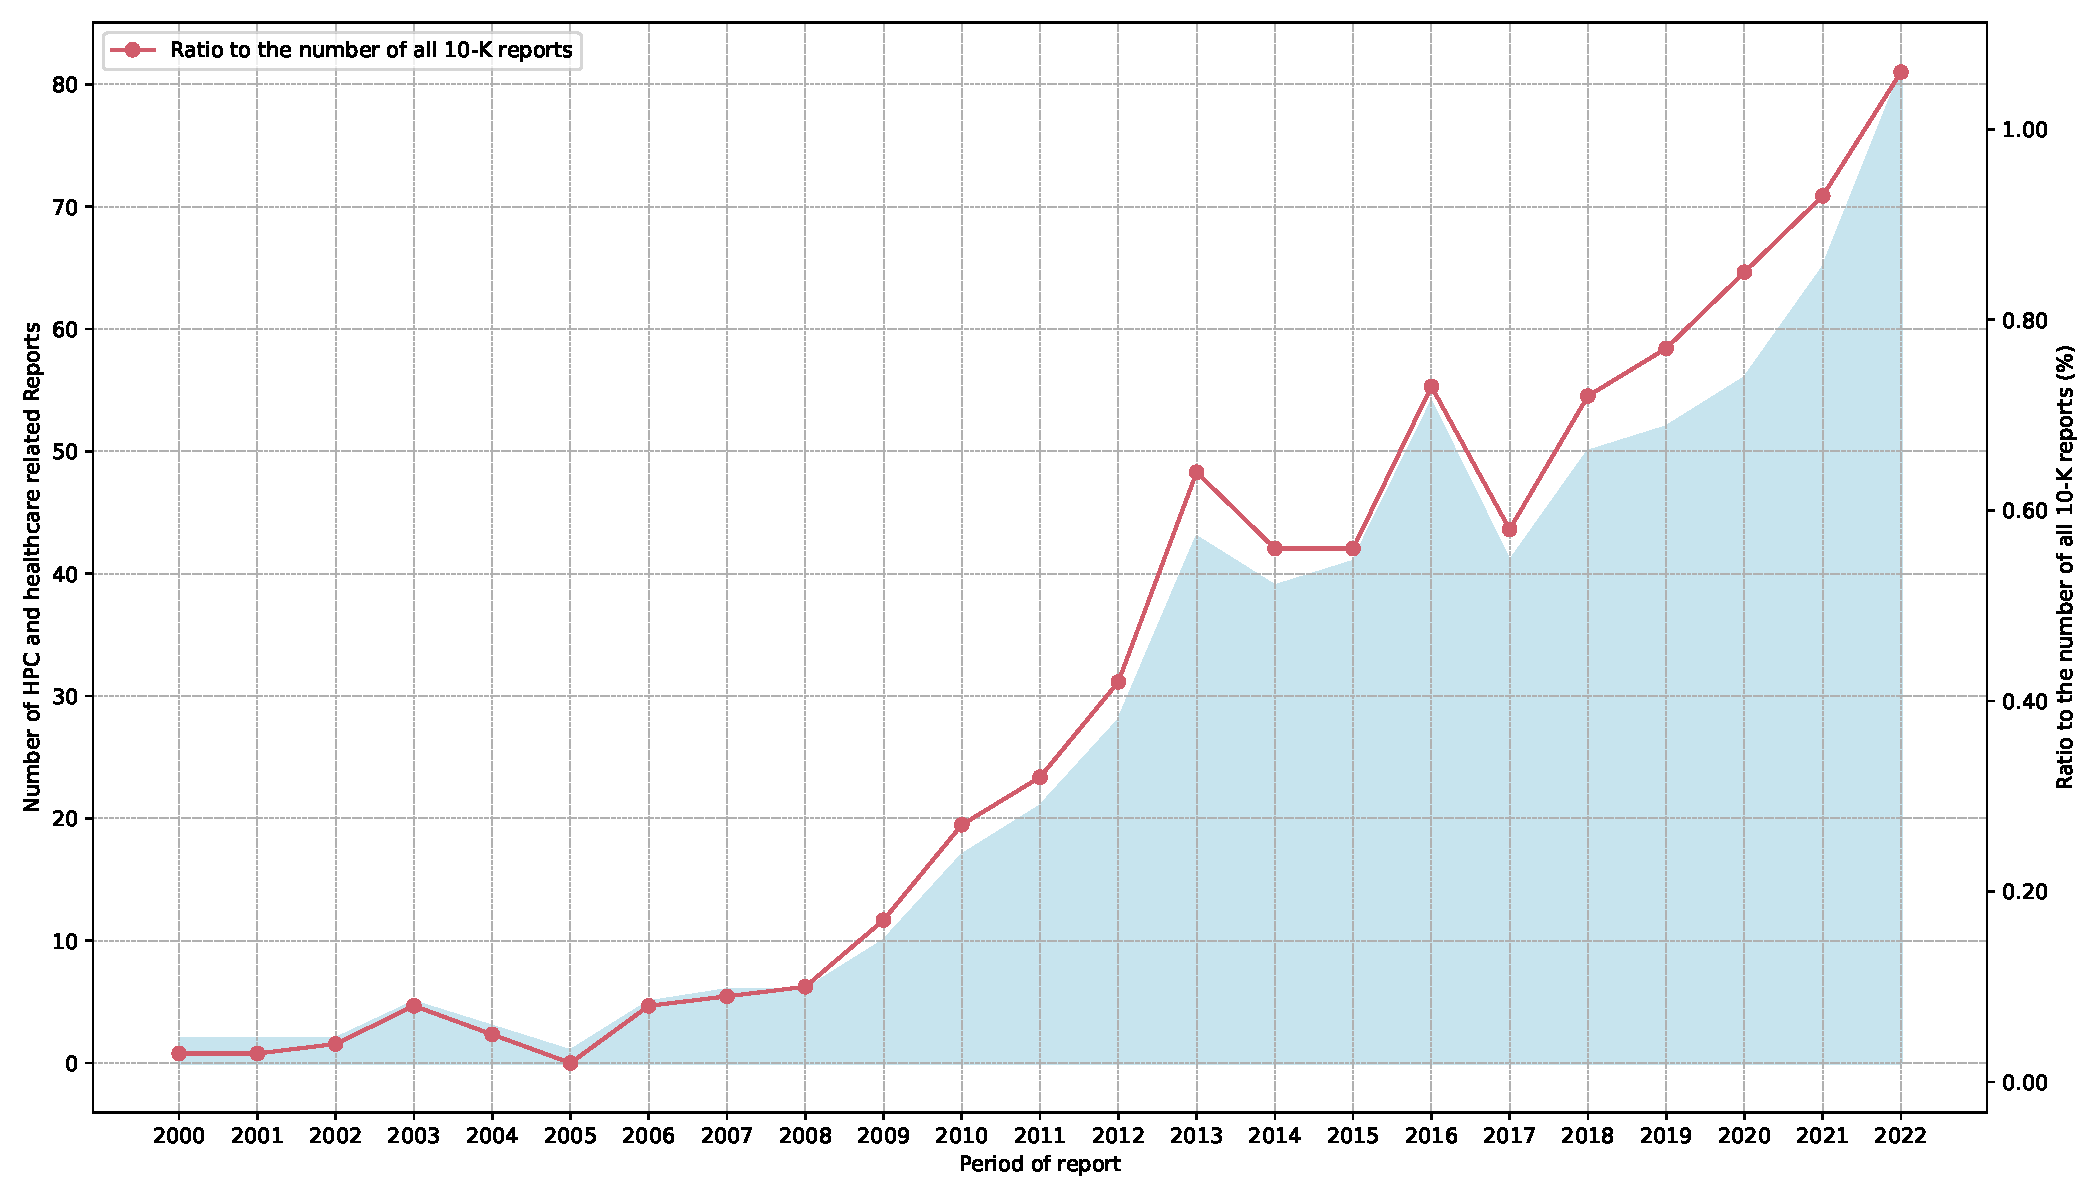
\includegraphics[width=0.95\textwidth]{5-4.pdf}
\caption{Absolute number of  HPC and healthcare-related 10-K reports according to years and also the ratio to the number of all 10-K reports filled that year}
\label{fig:5-4}
\end{figure}

\subsection{Value proposition transition}\label{subsec3.2}
\subsubsection{Value proposition transition pre- and post-HPC adoption}\label{subsec3.2.1}

The adoption of HPC by companies in the healthcare sector has brought a significant transition in terms of value proposition. The largest share of value propositions remains deeply rooted in the medical and clinical segment, underscoring a steadfast commitment to core healthcare services. However, there's a notable shift toward embracing cutting-edge technologies, evidenced by an 88\% increase in companies extending their operations into the data analytics and AI domains (panel (a) of Figure~\ref{fig:5-5}). The floating ratio is computed by subtracting the number of companies in specific topics before and after HPC adoption, then dividing by the number of companies before HPC adoption, based on the transition matrix. Section A.2 of the Appendix presents an example of a transition matrix from the value proposition perspective and illustrates how the chord diagram and floating ratios are generated based on it. This transition suggests an industry-wide recognition of the transformative potential of data-driven insights and in enhancing patient care and operational efficiency. To validate our observations, we examined the 10-K report of specific companies that underwent this transition. For instance, NEXTGEN HEALTHCARE, INC. (CIK: 708818), which demonstrated a shift from a clinically focused value proposition to business driven by data analytics.  Our analysis revealed that before 2009, NEXTGEN primarily developed and marketed healthcare information systems for physicians, hospitals, community health centers, and medical and dental schools. From 2009 onwards, after introducing web-based Software as a Service (SaaS) solutions for medical and dental practices, NEXTGEN pivoted to providing cloud-based healthcare technology solutions across the U.S. healthcare system. The 2022 10-K report highlights data analytics and value-based care as central to their value proposition. Additionally, the report indicates that recurring revenues, which include subscriptions to integrated cloud solutions, support, maintenance, and data services, rose to 90.5\% of total revenues in 2022.

Moreover, the core number of companies engaged in strategic and innovation consulting has remained stable, with a third of these companies now incorporating data analytics and AI into their offerings(panel (b) of Figure~\ref{fig:5-5}). This indicates a strategic integration of cutting-edge technologies to support traditional consulting services, enhancing their value proposition in an increasingly competitive market. For example, our analysis noted a business transition at Sandbridge Acquisition Corporation (CIK:1816708) from strategic management to data analytics. A review of their historical 10-K reports shows that before 2022, the company primarily focused on asset acquisition, reorganization, and investment. Following a merger with Owlet Baby Care Inc, Sandbridge was rebranded as ``Owlet, Inc.," marking a shift towards providing cloud-based infant monitoring solutions for parents. Additionally, a 32\% rise in companies expanding into access and network security highlights a growing prioritization of data protection. (panel (c) of Figure~\ref{fig:5-5}). This increased focus reflects a broader industry trend towards safeguarding patient information and ensuring compliance with stringent data protection regulations.

Notably, there's been a 44\% decline in companies primarily focused on manufacturing (panel (d) of Figure~\ref{fig:5-5}), suggesting a strategic pivot from traditional, product-centric models to service-oriented solutions. This shift from manufacturing to services, particularly those enhanced by HPC, data analytics, AI, and cybersecurity measures, underscores a response to the evolving healthcare landscape. Companies are moving away from hardware and toward integrated, technologically advanced services that offer greater value in today's digital and data-centric healthcare environment.


\begin{figure}[!h]
\centering
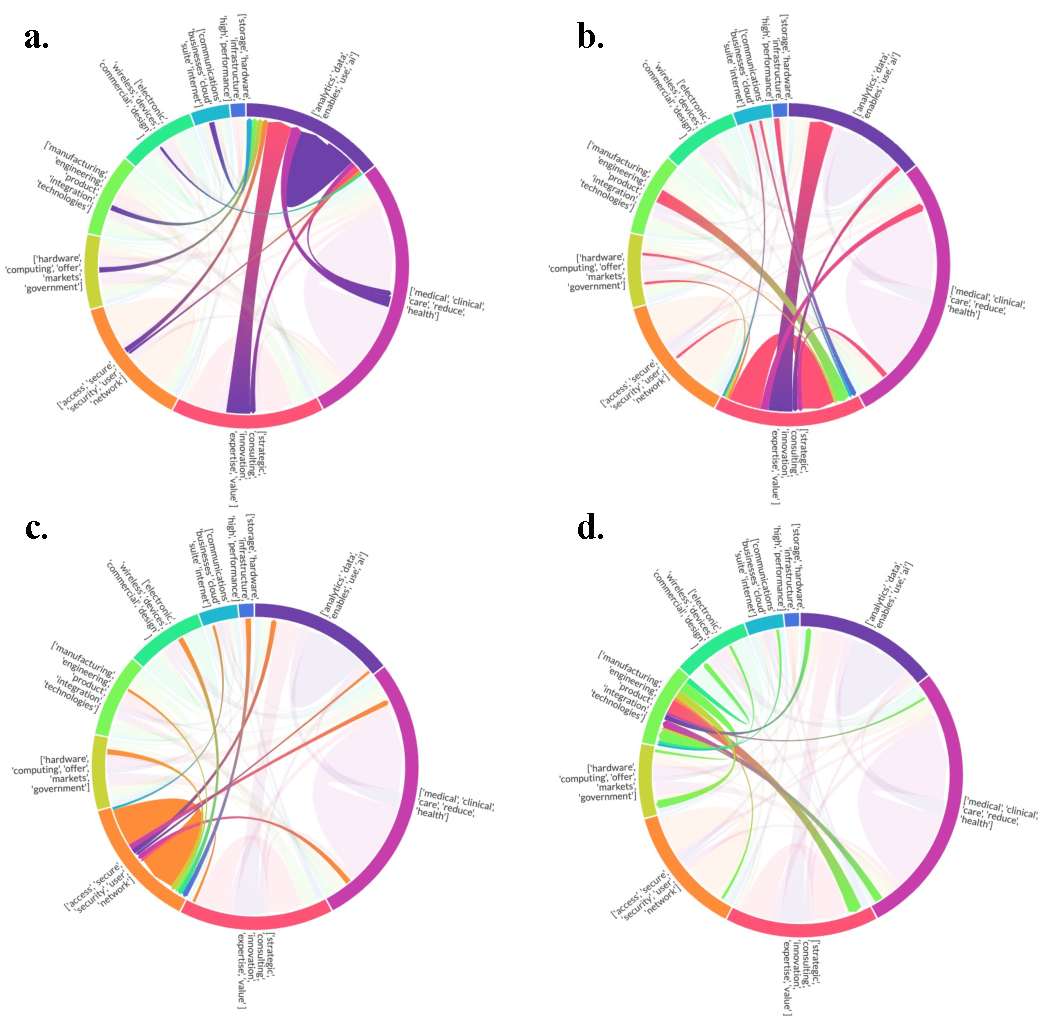
\includegraphics[width=0.95\textwidth]{5-5.pdf}
\caption{Visualizatio of value proposition transition. (a) 88\% increase in companies diversifying into data analytics and AI, (b) The number of companies focus on strategic and innovation consulting remains stable, but 33\% of these companies are also incorporating data analytics and AI into their services, (c) 32\% increase in companies expanding into access and network security, (d) 44\% decrease in companies primarily focusing on manufacturing.}
\label{fig:5-5}
\end{figure}

\subsubsection{Identify emerging value proposition trends in HPC adoption in healthcare over time}\label{subsec3.2.2}

In addition to observing the transition in value propositions for companies before and after HPC adoption, it is valuable to investigate the emerging trends of value propositions over time. To achieve this, we extract value propositions from all historical 10-k reports of companies operating in the healthcare sector that adopted HPC at certain years and employ topic modeling techniques. Figure~\ref{fig:5-6} highlights emerging trend-related topics such as novel oncology therapies, IoT, cybersecurity, and AI, as evidenced by the significant increase in the number of reports focusing on these topics since 2010. Furthermore, we identify companies associated with these emerging topics and analyze their performance over time. For instance, Merck \& Co., Inc. (CIK:310158), identified from the topic of novel oncology therapies, is one of the pioneers in computer-aided drug design since 1981 and has made significant investments in on-premises general purpose GPU technology in their strategy and roadmap~\cite{brown2017evolution}. Analysis of historical financial data from Compustat\footnote{\url{https://wrds-www.wharton.upenn.edu/pages/get-data/compustat-capital-iq-standard-poors/}} reveals that Merck's net profit margin (NPM) increased significantly to 21\% in 2019, with a return on investment (ROI) of 19\%. Furthermore, NPM increased to 25\% and 24\% in 2021 and 2022, respectively, while ROI remained stable around 18\% and 19\%. Additionally, Merck's stock price rose from \$23 in 2010 to \$130 in 2024. Ontrak, Inc. (CIK:1136174), an AI-powered and telehealth-enabled healthcare company specializing in personalized care programs, has experienced significant revenue growth since 2018, with growth rates of 97\%, 131\%, and 136\% in 2018, 2019, and 2020, respectively, indicating substantial business expansion. Similarly, DIGI INTERNATIONAL INC (CIK:854775), a leading global provider of business and mission-critical IoT connectivity products, contributes to enhanced patient outcomes and hospital operations through its provision of resilient and secure wireless connectivity. Since 2018, the company has maintained an average revenue growth rate of 16\%, accompanied by a steady increase in stock price from \$9.6 to \$32.6 since 2010. These positive company financial performances corroborate the role of HPC in facilitating shifts in novel value propositions and accelerating business growth.

\begin{figure}[!h]
\centering
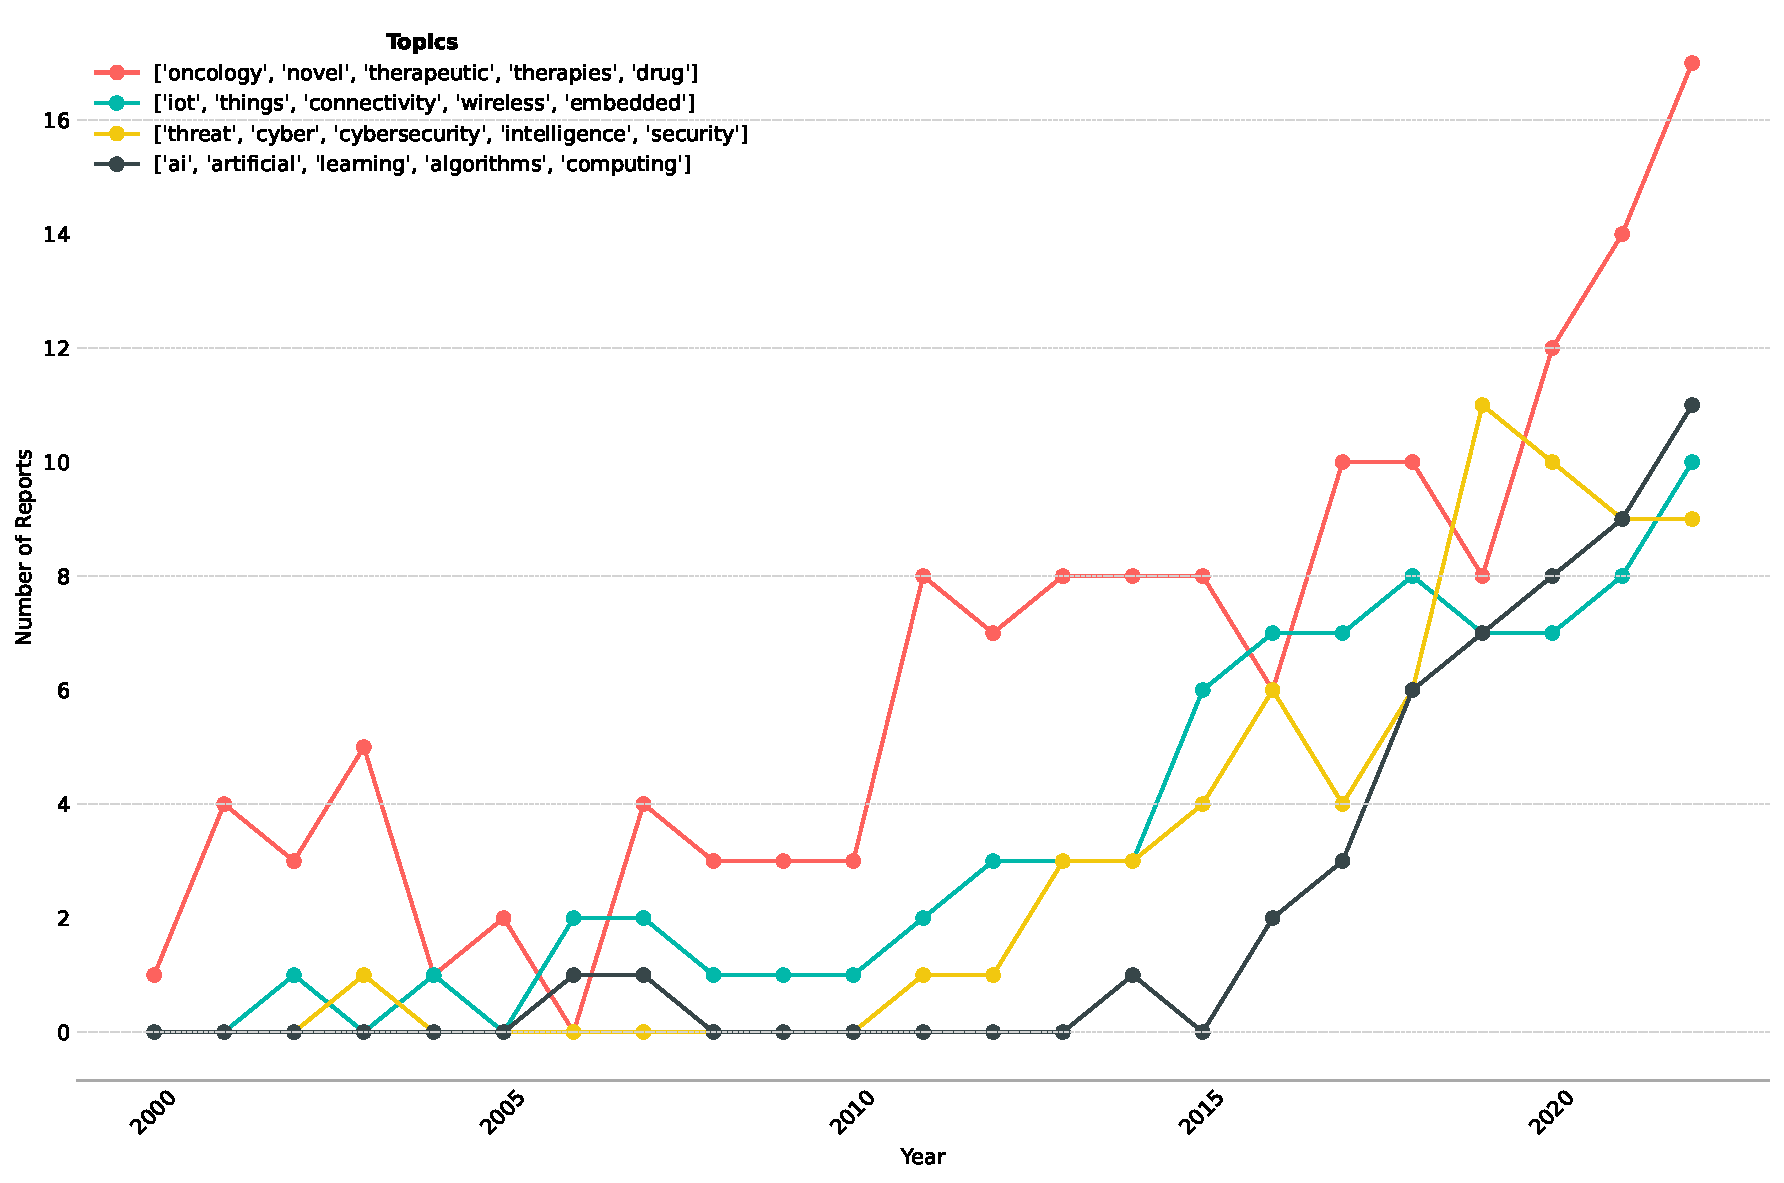
\includegraphics[width=0.95\textwidth]{5-6.pdf}
\caption{Line graph illustrating emerging trends of value proposition in HPC adoption in healthcare over time.}
\label{fig:5-6}
\end{figure}

\subsection{Customer segmentation transition}\label{subsec3.3}

HPC also substantially transforms approaches to customer segmentation, indicating a strategic shift towards diversification and expansion of customer bases. An impressive 85\% increase in companies targeting their services directly to patients underscores a transition towards a more patient-centric approach(panel (a) of Figure~\ref{fig:5-7}). This shift reflects a broader industry trend towards personalized healthcare, where advanced computing capabilities enable more tailored and efficient patient care solutions. Moreover, there's an 80\% rise in companies engaging with Small and Medium Enterprises (SMEs), indicating an expansion into serving businesses that are integral to the healthcare ecosystem, possibly through specialized services or technologies (panel (b) of Figure~\ref{fig:5-7}). About 41\% more companies have also started targeting organizations in the financial and insurance sectors related to life sciences (panel (c) of Figure~\ref{fig:5-7}), reflecting a strategic initiative to address the comprehensive needs of the healthcare industry, including financing and risk management. Additionally, the expansion into government and federal agencies, with a 20\% increase in companies targeting this segment (panel (d) of Figure~\ref{fig:5-7}), suggests a response to the growing opportunities in public health initiatives and regulatory compliance solutions.

\begin{figure}[!h]
\centering
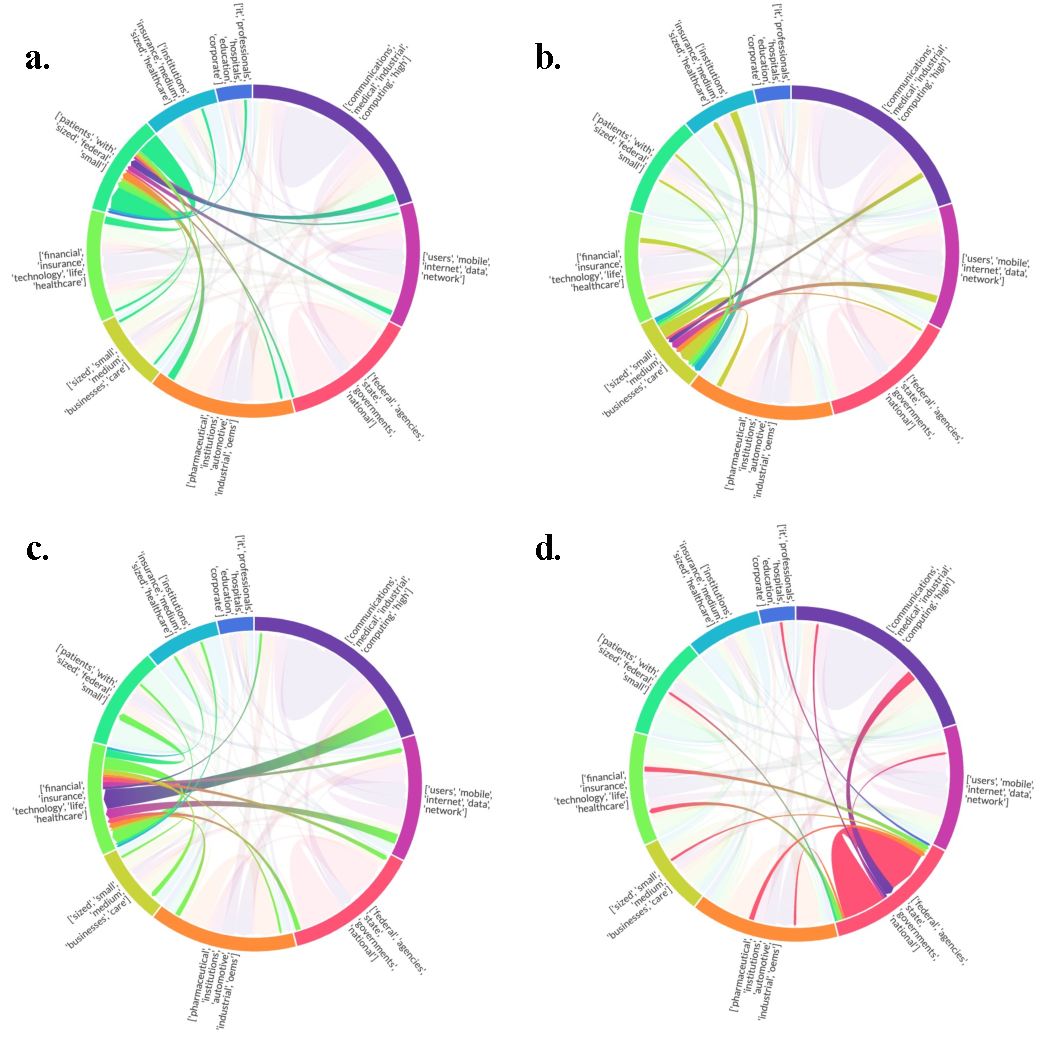
\includegraphics[width=0.95\textwidth]{5-7.pdf}
\caption{Visualizatio of customer segment transition. (a) 85\% increase in companies expanding their customer base directly to patients, (b) The number of company expanded their customer segment to SMEs increased  80\% (c) 41\% more companies catering to specialized sectors such as organizations operating in the financial, insurance relate to life sciences (d) 20\% increase in companies expanding their customer base to government/federal agencies.}
\label{fig:5-7}
\end{figure}

\subsection{Revenue stream transition}\label{subsec3.4}

Following the exploration of customer segment shifts, the landscape of revenue streams for healthcare companies reveals a significant evolution post-HPC adoption. This evolution marks a deliberate move towards more innovative and resilient financial models. The adoption of cloud computing has notably surged, evidenced by a 107\% increase in companies deriving their main revenue from cloud systems sales and maintenance (panel (a) of Figure~\ref{fig:5-8}). This trend highlights a strategic embrace of cloud computing's flexibility and scalability, crucial for managing the extensive data demands of modern healthcare. Furthermore, a 67\% rise in firms adopting subscription models underscores a growing preference for steady, recurring revenue streams (panel (b) of Figure~\ref{fig:5-8}). This shift towards subscription-based services reflects the sector's need for financial stability and continuous service enhancement, enabled by the ongoing advancements in HPC. The decrease in reliance on government and federal funding, with a 24\% drop in companies primarily funded by such means, suggests a strategic pivot towards the private sector and more diversified revenue sources (panel (c) of Figure~\ref{fig:5-8}). This movement is indicative of a broader desire to capitalize on the opportunities presented by HPC, steering away from traditional, less flexible funding models towards more dynamic and sustainable financial frameworks.

\begin{figure}[!h]
\centering
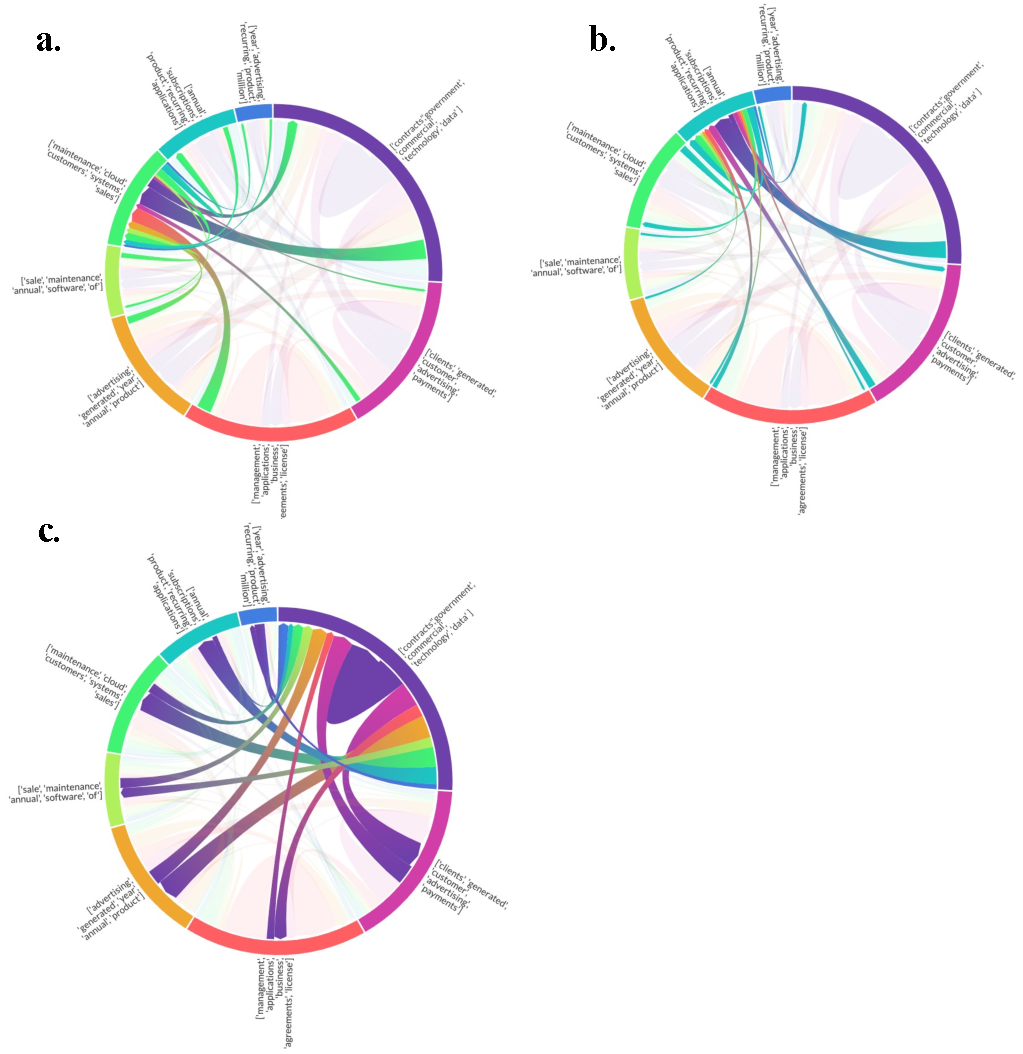
\includegraphics[width=0.95\textwidth]{5-8.pdf}
\caption{Visualization of revenue stream transition. (a) 107\% increase in the number of companies with main revenue stream from cloud systems sales/maintenance, (b) 67\% increase in the number of companies with main revenue stream from application subscriptions, (c) 24\% decrease in the number of companies with main revenue stream from government and federal agencies. }
\label{fig:5-8}
\end{figure}

\subsection{Cost structure transition}\label{subsec3.5}

In terms of cost structure perspective, a notable 47\% increase in operational costs reflects the substantial investments companies are making to refine their business models and enhance operations (panel (a) of Figure~\ref{fig:5-9}). These investments, while elevating short-term expenses, are aimed at harnessing the power of HPC for more efficient data processing and improved healthcare outcomes. Additionally, there's a 28\% rise in expenses related to data management and regulatory compliance (panel (b) of Figure~\ref{fig:5-9}), highlighting the complexities and costs associated with handling and securing large volumes of health data in an increasingly regulated environment.

Conversely, a 50\% reduction in manufacturing-related costs aligns with a strategic departure from traditional manufacturing towards more digital and service-oriented models (panel (c) of Figure~\ref{fig:5-9}). The shift away from manufacturing underscores a wider industry trend towards digital solutions and services, which, although lowering manufacturing costs, requires new investments in technological infrastructure and capabilities.

\begin{figure}[!h]
\centering
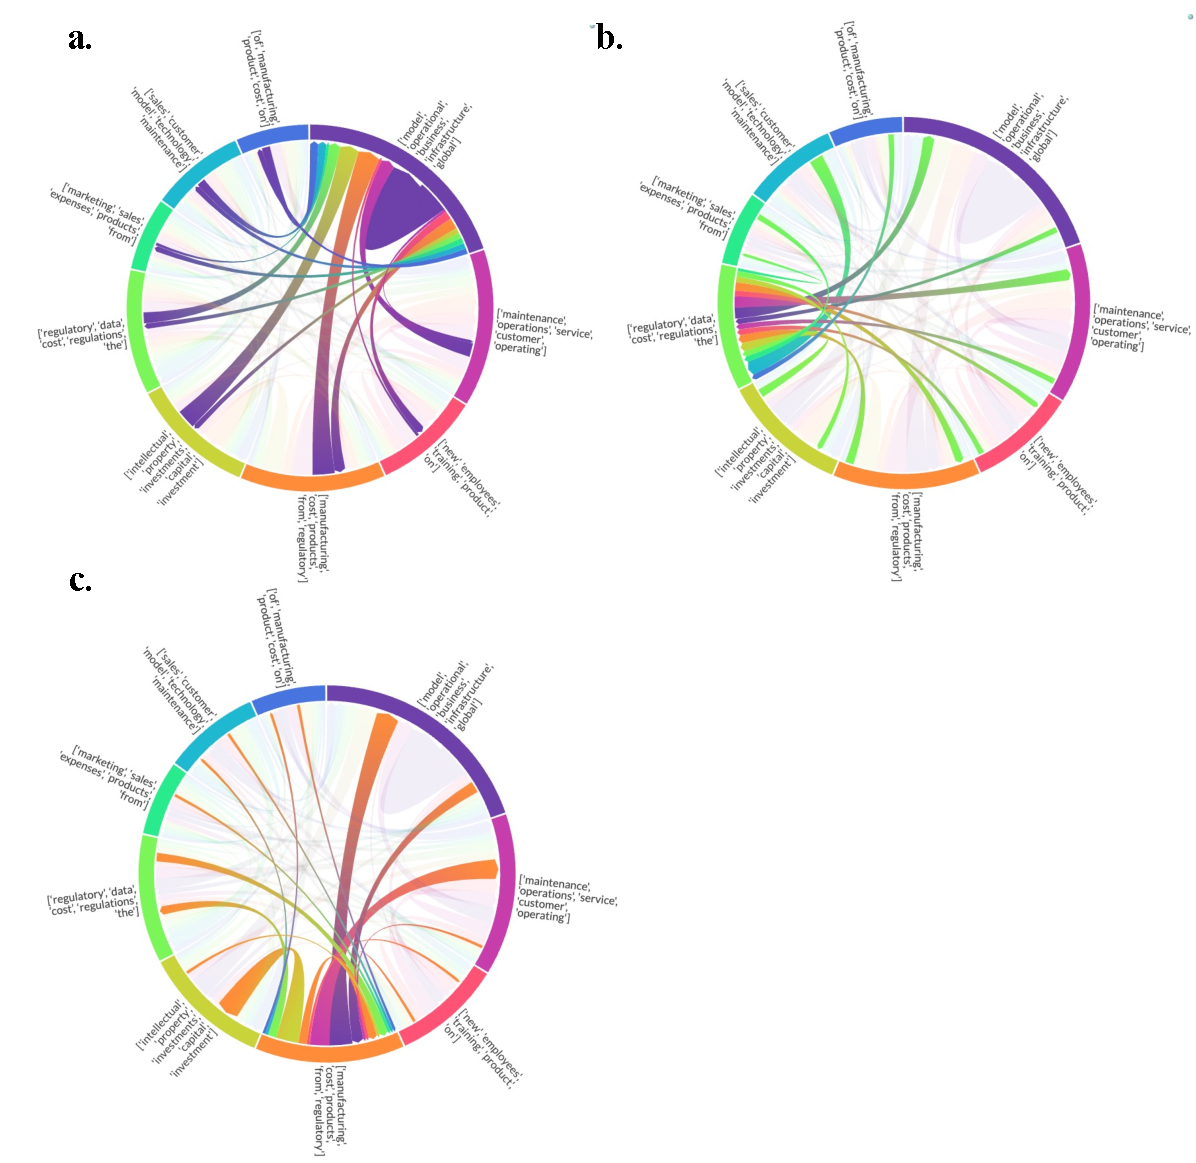
\includegraphics[width=0.95\textwidth]{5-9.pdf}
\caption{Visualization of cost structure transition. (a) 47\% increase in the number of companies whose primary cost structure is associated with business model refinement and operations, (b) 28\% increase in the number of companies whose primary cost structure is associated with data and regulation management. (c) 50\% decrease in the number of companies whose primary cost structure is associated with manufacturing.}
\label{fig:5-9}
\end{figure}

\subsection{Key activities  transition}\label{subsec3.6}

A significant observation is the 56\% increase in companies focusing on strategic technology implementation (panel (a) of Figure~\ref{fig:5-10}). This surge underscores the healthcare sector's recognition of the critical role technology plays in maintaining competitive advantage and addressing the complex challenges of modern healthcare delivery. Companies are investing more in integrating sophisticated technologies, such as HPC, to enhance their operational efficiency, data analytics capabilities, and ultimately, patient care services. Furthermore, there's been a 38\% increase in the emphasis on providing high-tech solutions and applications (panel (b) of Figure~\ref{fig:5-10}). This reflects a response to the healthcare industry's rapidly evolving technological needs, where there's a growing demand for advanced solutions that can process large volumes of data, support complex simulations, and deliver personalized patient care. The focus on high-tech solutions signifies a broader industry trend towards innovation and the adoption of cutting-edge technologies to meet the sophisticated needs of healthcare providers and patients alike.

\begin{figure}[!h]
\centering
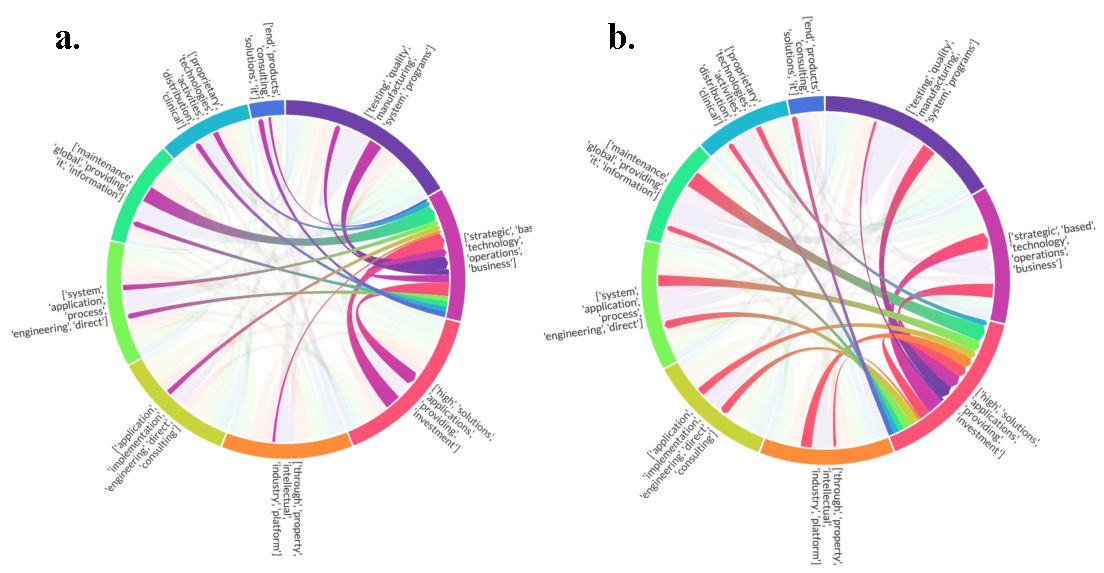
\includegraphics[width=0.95\textwidth]{5-10.pdf}
\caption{Visualization of key activities transition. (a) The number of company focus on strategic technology Implementation increased around 56\%, (b) 38\% increase in focus on providing high tech solutions.}
\label{fig:5-10}
\end{figure}

\subsection{Key resources  transition}\label{subsec3.7}

In terms of key resource perspective. a notable 42\% increase in companies identifying hardware and analytics tools as vital resources  (panel (a) of Figure~\ref{fig:5-11}), signifying the critical role of technological infrastructure in enabling data-driven healthcare solutions. This adjustment reflects a broader industry movement towards using computational power and analytical capabilities to process vast datasets. Moreover, the valuation of data as a key resource has escalated by 60\% (panel (b) of Figure~\ref{fig:5-11}), demonstrating the healthcare sector's increasing acknowledgment of data's essential role in enhancing care, advancing research, and encouraging innovation. This evolution emphasizes the strategic significance of data management and analysis capabilities.

Additionally, the changing dynamics around intellectual property, with a 29\% decline in the emphasis on trademarks and patents contrasted with a 13\% uptick in the valuation of other intellectual properties like product portfolios (panel (c and d) of Figure~\ref{fig:5-11}), indicate a nuanced shift in protecting and leveraging innovations. This evolution suggests a strategic realignment towards a broader conception of intellectual property, valuing comprehensive solutions and services that are increasingly vital in a technologically advanced healthcare ecosystem.

\begin{figure}[!h]
\centering
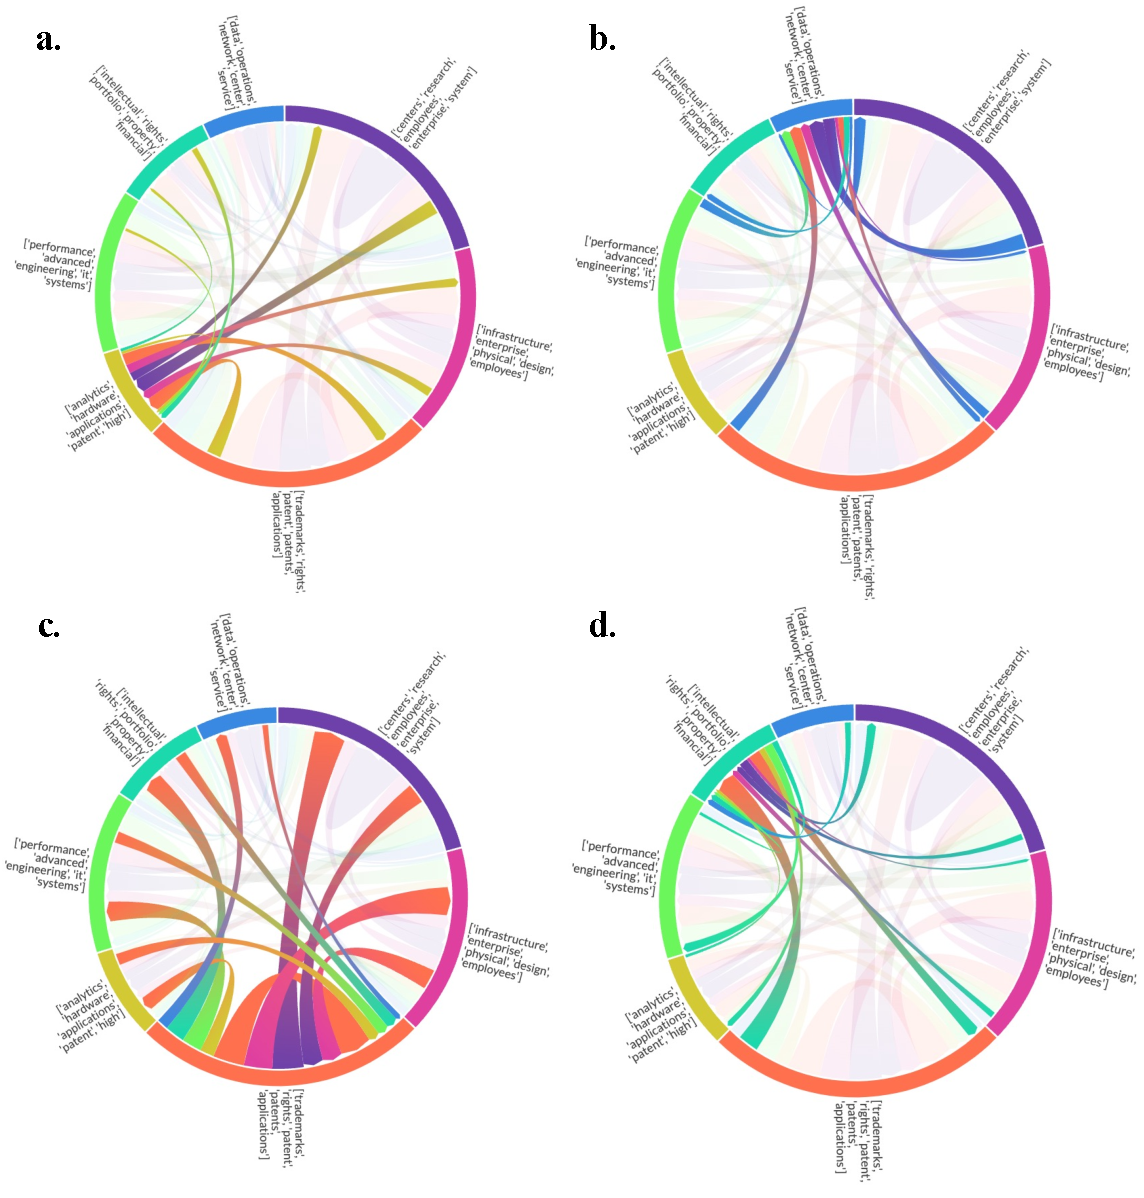
\includegraphics[width=0.95\textwidth]{5-11.pdf}
\caption{Visualization of key resources transition. (a) 42\% increase in companies treating hardware and analytics applications as key resources, (b) 60\% increase in valuing data as a key resources, (c) 29\% decrease in prioritizing trademarks and patents as key resources, (d) 13\% increase in valuing other intellectual properties like product portfolios as key resources.}
\label{fig:5-11}
\end{figure}


\section{Learning from the impact of HPC on business models in healthcare and identifying future opportunities}\label{sec4}

The ongoing business model transition within the healthcare industry is fundamentally a response to the technological revolution and the imperative to meet the evolving demands of healthcare delivery. The infusion of High-Performance Computing (HPC) is one of the catalysts for this shift, which is redefining the operational, strategic, and competitive landscape of healthcare businesses. This transition is characterized by a holistic shift towards technology and data-driven models, as evidenced by the industry's adoption of AI, data analytics, and cloud computing. These technological advancements have catalyzed a patient-centric approach, with healthcare companies broadening their market scope to engage directly with patients and diversifying their customer base. This strategic pivot is reshaping the operational framework and also redefining the nature of key resources, where the emphasis has shifted from physical assets to the valorization of data and intellectual property. The trend towards recurring revenue models is indicative of this transformation, reflecting a move away from traditional reliance on government funding and contracts towards more sustainable and predictable income streams. This technological shift is occurring because it aligns with broader trends of digitization and datafication that characterize contemporary economic and social environments. Businesses are compelled to transition not only due to the intrinsic benefits of technology but also to stay in step with these macro trends.

This transition is rooted in the pressing need for healthcare systems to become more efficient, cost-effective, and tailored to individual patient needs. Traditional models, heavily reliant on one-size-fits-all approaches and non-recurring revenue streams, are becoming obsolete in the face of personalized medicine and continuous care paradigms. Moreover, the push towards value over volume in healthcare reimbursement models encourages companies to invest in technologies that enhance patient outcomes and streamline operations. The evolution of revenue streams away from government or contract funding towards more predictable and stable sources underscores this strategic shift.

Looking forward, the incorporation of HPC is ready to unlock substantial opportunities for the healthcare industry. The shift from a one-time transactional model to ongoing, service-based relationships offers a platform for continuous innovation and improvement in patient care. Companies stand to gain from the development of new, data-centric business models that can adapt to and anticipate patient needs more effectively. Furthermore, as operational strategies lean more heavily on strategic technology investments, the potential for cross-sector collaborations and partnerships grows, potentially leading to a more integrated and efficient healthcare ecosystem. Protecting the increased volumes of sensitive data will also stimulate the growth of ancillary industries focused on cybersecurity and compliance, ensuring that the future of healthcare is not only technologically advanced but also secure and patient-focused.

\section{Discussion}\label{sec5}

In this study, we developed an automatic business model analysis framework by utilizing cutting-edge technologies such as LLM and the topic modeling technique Top2Vec. We applied this framework to analyze the impact of HPC on the business model transitions of companies in the healthcare domain, based on thousands of business reports. The interactive chord diagrams illustrate complex many-to-many relationships and transitions in an intuitive manner. This adaptable pipeline can be generalized to other domains by modifying the business report retrieval rules and will be beneficial for tracking and analyzing rapidly growing industries.

Due to the fact that 10-K reports are filed by all publicly traded companies within the United States, although many European or Asian-based companies are listed on U.S. stock exchanges, our analysis might potentially miss some entities operating in the HPC and healthcare-related domains. Secondly, our extraction of the BMC focuses on the business section (Item 1) of the 10-K report, as this section provides a comprehensive narrative of a company's ongoing operations and strategic directions. Its consistent and relevant data make it an ideal source for our analysis. Although other sections of the 10-K reports could also hold valuable information relate to business model, extracting the BMC from the entirety of thousands of 10-K reports using the GPT-4 model would be prohibitively costly and time-consuming. Consequently, our analysis concentrates on the business section of the 10-K reports.

One limitation of using topic models, like Top2Vec, is the need for human intervention to decide the optimal number of topics. This decision is subjective, relying on the analysis's specific context and objectives. The goal is to strike a balance between capturing the data's essential themes without creating too much overlap or too many divisions among topics. Thus, human insight and judgment are crucial in determining the right number of topics. To aid in this process, we utilize a dendrogram, which offers a more intuitive way to identify the ideal topic count.


Another issue with topic modeling is its lack of semantic understanding. Although topic models excel at detecting patterns in words and documents, they do not grasp the meanings behind the words. This shortfall can result in topics that are semantically inconsistent or challenging to interpret, necessitating manual review. One strategy to address this is through Entity Linking (EL), which adds a layer of explainability to topic modeling by connecting entities to a knowledge base, thereby enhancing topic interpretability~\cite{dillan2023ldaviewer,10.1145/3126686.3126776}. EL clarifies ambiguities by distinguishing between identical names referring to different entities, thus sharpening the accuracy of topic clusters. However, despite the assistance topic modeling provides in sifting through extensive business reports, it cannot replicate the nuanced and contextual insights provided by researchers. It should be regarded as a supportive tool rather than a replacement for the detailed exploration of business models. Acknowledging these limitations, future research should focus on refining this method, improving topic interpretability, and investigating alternative evaluation techniques. Despite its challenges, topic modeling continues to be an invaluable asset for comprehending the expanding corpus of business reports.

In conclusion, we introduce an innovative automated framework for analyzing business reports, aimed at understanding the impact of HPC on the evolutionary pathways of business models within the healthcare sector. Our framework encompasses the entire process, from retrieving and analyzing business reports to generating visual representations that illustrate the evolution of business models from various perspectives, utilizing the BMC. This adaptable framework can be tailored to suit different industries by adjusting the rules for retrieving business reports. Through the implementation of this automated analysis framework, we examined the trends in business model evolution among companies in the healthcare sector adopting HPC. These findings provide valuable insights for guiding future investments and the strategic advancement of HPC within the healthcare industry.





%\bibliographystyle{plain}
%\bibliography{my_bibs.bib}


\RemoveLabels

\setstretch{\dnormalspacing}

\backmatter

\end{document}
